%Document vide aux normes de l'École nationale des Chartes
%crée par J.B. Camps
%Dernières modifications E. Rouquette (03/2025)

%%%%%%%%%%%%%%%%%%%%%% PRÉAMBULE


%%%%%%%%%%%%%% partie obligatoire du préambule
\documentclass[12pt,twoside]{book}
\usepackage{fontspec}
\usepackage{xunicode}
\usepackage{polyglossia}
\usepackage{epigraph}
\usepackage{graphicx}
\graphicspath{
	{img/}             
	{partie_1/img/}
	{partie_2/img/}    
	{partie_3/img/}
	{sources/img/}
}
\usepackage{marginnote}
\setmainlanguage{french}%indiquer la langue principale du document
%\setotherlanguage{} %indiquer les autres langues utilisée


%%%%%%%%%%%%%%%%%%%%%%%%%%%%%%%%% PACKAGES UTILISÉS

\usepackage{csquotes} % les guillemets français
\usepackage{lettrine} %faire une lettrine (pas obligatoire)


\makeatletter
\def\blx@bbxfile@enc{biblatex-enc/enc.bbx}
\def\blx@cbxfile@enc{biblatex-enc/enc.cbx}
\makeatother
\usepackage[style=biblatex-enc/enc,sorting=nyt,maxbibnames=10]{biblatex}%charger le style de l'EnC (téléchargeable ici https://ctan.org/pkg/biblatex-enc)
\addbibresource{sources/memoire.bib} %le fichier bibliograhique. Exemple de chemin à partir du dossier où se trouve le document maître:Exemple ./dossierA/fichier.bib
%\defbibheading{}{\subsection*{}} Si l'on veut changer le titre de la/les bibliographie(s)


%%%Faire un ou plusieurs index

%\usepackage{imakeidx} %pour faire un ou plusieurs index
%\makeindex %commande pour générer l'index


%RAJOUTEZ ICI VOS PACKAGES
\usepackage{amsmath}
\usepackage[font=small]{caption} 


%%%%%%%%%%%%%%%%%%%%%%%%%%%%%%%%% CONFIGURATION DE MISE EN PAGE

%%%%%% Les compteurs (sections, subsections, etc)


%%%%%% Les compteurs (sections, subsections, etc)
\renewcommand{\thesection}{\Roman{section}.}%On ne fait apparaître que le numéro de la section
\renewcommand{\thesubsection}{\arabic{subsection}.}%subsection en chiffres arabes
\renewcommand{\thesubsubsection}{\alph{subsubsection}.}%subsubsection en lettres minuscules
%Si l'on veut faire apparaître les subsubsection dans le table des matières (à commenter sinon)
\setcounter{tocdepth}{3}
\setcounter{secnumdepth}{3}  % La subsubsection (profondeur=3 dans la table des matières) apparait numérotée dans la TdM



%%%%%  Configurer le document selon les normes de l'école

\usepackage[margin=2.5cm]{geometry} %marges
\usepackage{setspace} % espacement qui permet ensuite de définir un interligne
\onehalfspacing % interligne de 1.5
\setlength\parindent{1cm} % indentation des paragraphes à 1 cm


%%%%% Mise en forme des headers (haut de page)

\usepackage{fancyhdr} %package utilisé pour modifier les headers
\pagestyle{fancy} %utiliser ses propres choix de mise en page et non ceux par défaut du package

\setlength\headheight{16pt}%la hauteur des headers

%%la façon dont les sections apparaissent dans les en-tête:

\renewcommand{\sectionmark}[1]{\markright{\small\textit{\thesection~\  #1}}}%Faire apparaître dans les headers les sections en  petit et en italiques
%\renewcommand{\sectionmark}[1]{}%Commenter la lign précédetne et mettre celle-ci pour ne pas avoir le titre des sections dans le header

%% réglages propres à frontmatter

\appto\frontmatter{\pagestyle{fancy}%
	\renewcommand{\chaptermark}[1]{\markboth{\small\textit{#1}}{}}% ne pas faire apparaître de <<numéro>> de chapitre dans les chapitres non numérotés (front: l'introduction, els remerciement, etc)
}

%% réglages propres à mainmatter

\appto\mainmatter{
\renewcommand{\chaptermark}[1]{\markboth{\small\chaptername~\thechapter~--\ \textit{#1}}{}}%faire apparaître dans les headers les sections en  petit et en italiques
%\renewcommand{\chaptermark}[1]{}%Commenter la ligne précédente et mettre celle-ci pour ne pas avoir le titre des chapitres  dans le header
}

%% réglages propres aux annexes

\appto\appendix{
	\renewcommand{\chaptermark}[1]{\markboth{\small~Annexe \thechapter~--\ \textit{#1}}{}}%faire apparaître dans les headers le nom des annexes
	%\renewcommand{\chaptermark}[1]{}%Commenter la ligne précédente et mettre celle-ci pour ne pas avoir le titre des chapitres  dans le header
}




%indiquer des règles d'hyphénation pour des mots précis si besoin
%\begin{hyphenrules}{french}
%	\hyphenation{}
%\end{hyphenrules}


%%%%%%% Package hyperref

% A mettre après les autres appels de packages car redéfinit certaines commandes).

\usepackage[colorlinks=false, breaklinks=true, pdfusetitle, pdfsubject ={Mémoire HN}, pdfkeywords={les mots-clés}]{hyperref} %
\usepackage[numbered]{bookmark}%va avec hyperref; marche mieux pour les signets. l'option numbered: les signets dans le pdf sont numérotés

% Compléter pdfsubjet et pdfkeywords
%Explication des options de hyperref (modifiables)
% hyperindex=false
% colorlinks=false: pour que le cadre des liens n'apparaisse pas à l'impression
% breaklinks permet d'avoir des liens allant sur pusieurs lignes
%pdfusetitle: utiliser \author et \title pour produire le nom et le titre du pdf


%avec overleaf, utiliser :
%\usepackage[xetex]{hyperref}
%\hypersetup{
	%	pdfauthor = {Prénom Nom},
	%	pdftitle = {titre},
	%	pdfsubject = {sujet},
	%	pdfkeywords = {premier mot-clé} {deuxième mot-clé} {troisième mot-clé} {etc}
	%}
\hypersetup{
	breaklinks=true % pour couper le lien sur plusiru lignes
}



%%%%%%%%%%%%%%%%%%%% Package glossaries

%Exception: il faut le charger APRÈS hyperref
%\usepackage[toc=true]{glossaries}
%\makeglossaries
%avec TexStudio: F9 pour compiler le glossaire (s'il y a aussi un index)

%mettre les entrées du glossaire ici ou les mettre dans un fichier à part que l'on appelle ici par \loadglsentries{nom_du_fichier.tex}

%Structure d'une entrée de glossaire
%\newglossaryentry{}{%
%	name={},%
%	description={}
%}



%%%%%%%%%%%%%%%%%% DÉFINITION DES COMMANDES ET ENVIRONNMENTS

\usepackage{tcolorbox}

\newtcolorbox{encadre}[1][]{%
	colback=blue!5!white,
	colframe=blue!75!black,
	fonttitle=\bfseries,
	title=Point technique,
	arc=4pt,
	left=6pt,
	right=6pt,
	top=6pt,
	bottom=6pt,
	fontupper=\fontsize{9}{10}\selectfont
}




 %%%%%%%%%%%%%% INFORMATIONS POUR LA PAGE DE TITRE
 
\author{Joël \textsc{Féral} - M2 TNAH}
\title{L'outil Mezanno pour les approches quantitatives en sciences humaines et sociales. De l'élaboration d'un corpus de documents sériels à l'extraction automatisée de données structurées: les tables annuelles du \hbox{Journal Officiel} (1931 - 1935) comme cas d'usage}

%%%%%%%%%%%%%%%%%%%%%% DOCUMENT
\begin{document}
	\begin{titlepage}
		\begin{center}
			
			\bigskip
			
			\begin{large}				
				ÉCOLE NATIONALE DES CHARTES\\
				UNIVERSITÉ PARIS, SCIENCES \& LETTRES
			\end{large}
			\begin{center}\rule{2cm}{0.02cm}\end{center}
			
			\bigskip
			\bigskip
			\bigskip
			\begin{Large}
				\textbf{Joël Féral}\\
			\end{Large}
		%selon le cas
			\begin{normalsize} \textit{licencié ès lettres}\\
				\textit{diplômé de master}
			\end{normalsize}
			
			\bigskip
			\bigskip
			\bigskip
			
			\begin{Huge}
				\textbf{L'outil Mezanno pour les approches quantitatives en sciences humaines et sociales}\\
			\end{Huge}
			\bigskip
			\bigskip
			\begin{LARGE}
				\textbf{De l'élaboration d'un corpus de documents sériels à l'extraction automatisée de données structurées: les tables annuelles du \hbox{Journal Officiel} (1931 - 1935) comme cas d'usage}\\
			\end{LARGE}
			
			\bigskip
			\bigskip
			\bigskip
			\begin{large}
			\end{large}
			\vfill
			
			\begin{large}
				Mémoire 
				pour le diplôme de master \\
				\enquote{Technologies numériques appliquées à l'histoire} \\
				\bigskip
				2025
			\end{large}
			
		\end{center}
	\end{titlepage}

	\thispagestyle{empty}	
	\cleardoublepage
	
\frontmatter

	\chapter{Résumé}
\medskip
	Résumé du mémoire en français. Cette page ne doit pas dépasser une page.\\
	
	\textbf{Mots-clés:} Journal Officiel; Sénat; Génération structurée; LLM; Mezanno; séparés par des points-virgules.
	
	\textbf{Informations bibliographiques:} Prénom Nom, \textit{Titre du mémoire. Sous-titre du mémoire}, mémoire de master \enquote{Technologies numériques appliquées à l'histoire}, dir. [Noms des directeurs.trices], École nationale des chartes, 20245.
	
		\newpage{\pagestyle{empty}\cleardoublepage}
	
	\chapter{Remerciements}
	
\lettrine{M}es remerciements vont tout d'abord à Jean-Philippe M., Joseph C., Marie P. et Sébastien C. qui m'ont fait confiance pour participer à l'élaboration du projet Mezanno. 

Je remercie également mes parents ET SURTOUT DGETTO !!!
	\newpage{\pagestyle{empty}\cleardoublepage}
	

%%%%%%%%%%%%%%%%%%%%%%%% BIBLIO, BIBLIOGRAPHIE %%%%%%%%%%%%%%%%%%%%%%%%%
%%%%%%%%%%%% \bibliographie ici (normes de l'EnC)

\printbibheading[heading=bibintoc]
\printbibliography[heading=subbibintoc,keyword=archivistique,title=Méthodologie historique]
\printbibliography[heading=subbibintoc,keyword=parlementaire,title=Droit\, Histoire et Actualité Parlementaire]
\printbibliography[heading=subbibintoc,keyword=pat,title=Institutions  et politiques patrimoniales]
\printbibliography[heading=subbibintoc,keyword=hn,title=Humanités numériques]
\printbibliography[heading=subbibintoc,keyword=Numérisation,title=Images et numérisation]
\printbibliography[heading=subbibintoc,keyword=tal,title=Traitement automatique du langage]
\printbibliography[heading=subbibintoc,keyword=archeologie,title=Philosophie de la technique et médialité]
\printbibliography[heading=subbibintoc,keyword=maths,title=Mathématiques]

%%%% réfs oubliées %%%%

\printbibliography[
heading=subbibintoc,
notkeyword=archivistique,
notkeyword=parlementaire,
notkeyword=pat,
notkeyword=hn,
notkeyword=Numérisation,
notkeyword=tal,
notkeyword=archeologie,
notkeyword=maths,
title={Oublis}
]

%%%%%%%%%%%%%%%%%%%%%%%%%%%%%%%%
%%%%%%%%%%%%%%%%%%%%%%%%%%%%%%%%
%%%%%%%%%%%%%%%%%%%%%%%%%%%%%%%%
%%%%%%%%%%%%%%%%%%%%%%%%%%%%%%%%
%%%%%%%%%%%%%%%%%%%%%%%%%%%%%%%%
%%%%%%%%%%%%BEGIN%%%%%%%%%%%%%%%
%%%%%%%%%%%%%%%%%%%%%%%%%%%%%%%%
%%%%%%%%%%%%%%%%%%%%%%%%%%%%%%%%
%%%%%%%%%%%%%%%%%%%%%%%%%%%%%%%%
%%%%%%%%%%%%%%%%%%%%%%%%%%%%%%%%
%%%%%%%%%%%%%%%%%%%%%%%%%%%%%%%%

\chapter{}
\vspace*{\fill} 
\epigraph{\itshape Remuer du papier ne peut pas être inutile.}{Bruno Latour}

\vfill\clearpage

	
\chapter{Introduction}	
Pour l'historien, les archives font figure centrale \footcite{boutier}. Pour répondre à une question de recherche, le chercheur va dépouiller, trier, classer, reclasser, recouper les documents ou les données issus de fonds ou de collections recueillies. Cette matière se constitue alors en corpus pour ajuster des questions ou charpenter des réponses. Dans l'épars documentaire s'esquissent des hypothèses, s'élaborent des solutions. L'information enfin extraite des cartons, des rayons ou des documents disponibles sur le Web peut être enfin convoquée, parfois après un laborieux travail de dépouillement. Avec un peu de chance, l'information s'offre presque toute prête : ainsi les lignes budgétaires de tel livre de compte de telle institution; ainsi telles entrées de tels annuaires professionnels. Tantôt il faudra reproduire manuellement l'information qui a été dénichée feuille à feuille et parfois photographiée à la hâte; tantôt, avec un peu plus de chance, simplement récupérer des jeux de données quasiment prêts à l'emploi et les traiter selon ce qu'exige les impératifs scientifiques. Une fois les données réunies en lignes et en tableaux, l'enquête ne fait que commencer: c'est qu'il s'agit de supposer des tendances, des points de comparaison; de dégager aux événements des séries ou des structures explicatives et forger des réponses. Ainsi la \enquote{centralité de l'archive} -- et des données -- dans le travail de l'historien.

Derrière ces masses de documents sériels, une allure : ce sont des bases de données de papier. Elles contiennent des noms et des nombres, des métiers ou des adresses. Pour le chercheur, ces sources répétitives se prêtent volontiers à une traduction numérique pour faciliter et opérer des traitements plus systématiques en bénéficiant des capacités calculatoires de l'ordinateur. Egalement pour l'archiviste en charge de l'indexation des fonds, elles regorgent de noms qu'il est intéressant d'exposer, par exemple, à son public de généalogistes via les portails de recherche d'archives. Naturellement, il est tentent d'employer l'outil informatique pour déléguer -- ou rendre possible -- ce travail d'extraction et de structuration de l'information présente dans les masses documentaires. Les grands modèles de langue (les \textit{LLM}) semblent pouvoir faire endosser aux ordinateurs ce labeur de traduction et de structuration de l'information. Se dessinent alors des enjeux techniques et épistémologiques d'un passage -- celui des documents \enquote{analogiques} aux données numériques -- qu'il convient d'interroger. 

Ce mémoire interroge la problématique de la traduction de ces corpus sériels en ensembles de données structurées, dans une perspective d’analyse historienne et archivistique. 
Historienne d'abord, car il s'agit d'explorer de \enquote{nouvelles frontières} disciplinaires impliquant la collaboration entre chercheurs en SHS, informaticiens et institutions patrimoniales en vue d'exploiter à des fins scientifiques des données issus de fonds numérisés; archivistique ensuite, car la traduction des informations contenues dans les documents en données exploitables par des systèmes informatiques rejoignent les enjeux d'indexation et donc de valorisation d'ensembles documentaires.

Cette problématique de traduction de fonds sériels en données structurées exploitables pour l'analyse quantitative historienne ou pour la valorisation documentaire part d’un constat : nombre de publications administratives ou normatives — annuaires, lois, décrets, tables parlementaires — relèvent d’une production sérielle à forte teneur informationnelle mais échappent aux catégories sensibles habituellement mobilisées dans le rapport aux archives. Leur lecture manuelle est difficile, leur dépouillement peut être décourageant. On s'éloigne ici du \enquote{goût de l'archive} d'Arlette Farge\footcite{farge} qui dépeint une phénoménologie sensible de la source historique pour adopter une approche moins solipsiste de valorisation de documents "sans goût" -- mais dont on aura restitué un pluriel. Ces fonds sériels -- dont il est difficile de valoriser au même titre que de prestigieuses chartes médiévales ou de précises gravures scientifiques étant donné leur monotone prosaïsme -- forment en effet une mémoire institutionnelle précieuse qu'il convient d'interroger dès lors qu’on parvient à les structurer et les croiser avec d’autres sources.

Si on n'arrête pas de louer depuis quelques décennies de nouveaux tournants dans la façon de travailler sur les sources grâce à l'outil numérique, il faut bien avouer que les derniers développements autour des grands modèles de langage accentuent un virage. La fouille de texte, la \enquote{lecture à distance} (\textit{distance reading})\footcite{distant}, et tout ce qui implique l'extraction d'information sémantique, reposent sur une récente synergisation des techniques numériques : tout d'abord, la capacité à restituer un objet physique en image discrète (numérisation); de structurer et normaliser l'accès à des images dans des dépôts centralisés via des protocoles HTTP(API); de retranscrire de l'image l'information textuelle (OCR) ou des structures de pages (Document Layout Detection); et de la structuration sémantique \textit{a posteriori} des entités nommées de façon semi-automatique -- moyennement un apprentissage supervisé via l'annotation ou le moissonnage de la production scientifique en ligne, déjà numérisée. Cette synergie des traitements sur l'image numérique et des développement en linguistique computationnelle renouvelle \enquote{les frontières de l'historien} en ce sens que, pour peu que les documents soient numérisées, on puisse automatiser le travail d'extraction de l'information présente dans les sources. La chaîne qui va de la numérisation du document à l'extraction de données sémantiquement structurées et son analyse via l'outil informatique forme un \textit{système technique}\footcite{meot} et l'historien, le sociologue ou encore le statisticien s'y inscrivent pleinement. 

Une précaution : la question technique qui participe de l'administration des nouvelles frontières de l'historien n'est pas seulement un moyen d'automatiser des tâches qui autrefois étaient plus manuelles : elle apporte dans ses rêts de nouveaux enjeux épistémologiques (les données ne se donnent pas, ce sont des \textit{capta}\footcite{drucker}), des manières de réactiver des questions ou des réponses\footcite[][]{prost}, des sources documentaires, des méthodes (impliquant un redivision du travail) ou des façons de travailler (Ladurie, l'historien et l'ordinateur). Les questions techniques sont moins une affaire d'automatisation que de sensibilité des systèmes techniques à l'information et leur relation avec le travail humain (Simondon). De même, les instruments ne font pas que servir le travail intellectuel de façon neutre : ils sont aussi de la \enquote{théorie réifiée} (Bachelard). Se superposent ainsi le champ énonciatif des systèmes techniques et des disciplines scientifiques qui s'y inscrivent et expriment des connaissances \textit{situées}. Les outils techniques promettent des méthodologies -- lesquelles reposent sur de manière d'envisager la division d'un travail pour une tâche déterminée. Les \textit{pipelines} de traitement de données -- de l'image au texte structuré -- se constituent à la fois comme outil et comme condensation \textit{in silicium} des \textit{a priori} épistémologiques. Les solutions techniques à des problèmes scientifiques sont une affaire de \textit{design}\footcite{renon}, c'est-à-dire de stratégies épistémiques et valuatives.


Dès lors, comment articuler les enjeux historiographiques propres à ces corpus avec les nouvelles opportunités d’extraction et de structuration automatiques qu’offrent les techniques récentes et leur synergisation ? (OCR, modèles de langage, outils d’annotation) ? Comment construire une chaîne de traitement reproductible, capable de restituer la richesse de ces fonds tout en garantissant la qualité des données produites ? La question de la valuation des méthodes -- c'est-à-dire de leur légitimité au regard de ce à quoi on tient savoir --, elle-même, semble dépendre des besoins : un archiviste n'a pas tout à fait les mêmes besoins qu'un historien -- et tous les historiens n'ont pas les mêmes besoins. Pour le premier, l'exactitude est de mise; pour le second qui adopte une approche statistique, des données fiables -- c'est-à-dire probablement imparfaites -- seront suffisantes pour effectuer des \enquote{pesées globales} historiques\footcite{muller}.


Ces questionnements auront été les miens durant mon stage à l'EPITA/BnF où j'ai eu l'occasion de travailler à la convergence des nouvelles opportunités de traitements automatiques et de la question de la légitimité épistémique de données produites par des systèmes techniques, à partir de l'extraction d'informations sous forme structurée du Journal Officiel de 1931, dans une optique de préparation de l'analyse des discours historiques sous la IIIe République. [à développer] 

Cette interrogation se décline ainsi selon ces trois axes :

\begin{itemize}
	\item Que sont les sources sérielles et quels sont leurs apports spécifiques pour répondre à une question de recherche ? En quoi leur structure, leur cumulativité et leur forme normative permettent-elles des lectures nouvelles, notamment en lien avec les pratiques de gouvernement et les dispositifs de publicité du droit sous la IIIe République ? Pour aborder ce point, je me pencherai sur l'analyse des Tables du Sénat de 1931 car, dans une perspective de \textit{reenactement} historien de l'activité parlementaire, elles donneraient un corps à cette problématique de traduction de sources sérielles en sources exploitables pour l'analyse.
	\item Quelles méthodes et quels outils permettent aujourd’hui d’en automatiser la structuration ? Comment construire un protocole d’extraction cohérent, tenant compte de la matérialité des documents (OCR, mise en page, bruit), des formats de sortie, et des finalités analytiques visées ?
	\item Comment évaluer la fiabilité des données ainsi produites et garantir leur légitimité scientifique ? Quels critères de qualité, de traçabilité et de transparence permettent de faire de ces résultats des objets d’enquête mobilisables par les historiens ?
\end{itemize}

A travers ces trois axes, qui constituent chacun une partie de ce mémoire, je veux donc répondre à la problématique du passage de l'information sérielle non-structurée présente dans les sources, à la fois sur des aspects documentaires; techniques (méthodes d'extraction) et valuatives (évaluation et épistémologie de l'évaluation).



\newpage{\pagestyle{empty}\cleardoublepage}

				%%%%%%%%%%%%%%%%%	Le corps du mémoire

\mainmatter

%%%%%%%%%%%% PARTIE 1
\part{Des sources sérielles: les Tables Annuelles du Sénat comme cas d'usage}

\chapter{Le \emph{Journal Officiel} : la parole, la main, la vue et le droit}

\enquote{Pas de question sans document. [La question de l'historien] n'est pas une question nue; c'est une question armée, qui porte avec elle une idée des sources documentaires et des procédures de recherches possibles}. \footcite[][80]{prost}. Ainsi, Antoine Prost, à partir des propositions de Robin G. Collingwood sur les questions historiques, expose l'idée d'une solidarité entre une question de recherche, les documents et les procédures de leur traitement. La question de l'historien, tout d'abord, est \enquote{armée} : cela signifie qu'elle ne vient pas seule pour satisfaire, avec désintéressement, une curiosité passagère; elle prend appui sur l'actualité de l'historien, de ce qui fait qu'elle puisse être pertinente socialement et scientifiquement. \enquote{Armée} : cela veut dire également que l'historien a déjà une idée des sources documentaires sur lesquelles travailler. Le chemin de la connaissance du passé, qui s'ouvre avec une question de recherche, est motivé par un \emph{reenactement}, une réactivation du passé depuis le présent. Par là, il s'agit d'être à l'écoute des \enquote{palpitations du temps} présent -- pour reprendre ce mot de l'historien de l'art Eugeni d'Ors \footcite[][]{ors} -- et de réinterroger l'actualité à travers des documents à explorer. \enquote{Il n'y a d'histoire que de choses pensées au présent par l'historien}\footcite[][p.166]{prost} : selon l'approche collingwoodienne -- qui n'est d'ailleurs pas sans rappeler la position de Walter Benjamin sur l'histoire comme \enquote{objet d’une construction dont le lieu n’est pas le temps homogène et vide, mais qui forme celui qui est plein de temps actuel} \footcite[][]{benjamin} -- la pratique historienne est une dialectique entre passé et présent. Les documents, alors, ne sont pas \enquote{un dépôt mort} mais une \enquote{énergie fossile} qui reffectue une pensée\footcite[][]{libera} et viennent renouveler un questionnaire. Les prétentions historiennes collingwoodiennes semblent alors aller au-delà d'une satisfaction strictement érudite -- ou du moins sans volitions éthiques -- pour atteindre la nécessité de réévaluer le passé avec des considérations toutes pragmatistes, c'est-à-dire valuatives\footcite[][]{dewey}. Si l'historien est lui-même un sujet situé historiquement et socialement, il est également saisi dans des configurations techniques qui peuvent changer ses procédures de recherche -- la numérisation de sources historiques et leur mise à disposition sur le Web étant un exemple assez criant. Le milieu de l'historien a donc lui-même une historicité; sociale, technique, psychique --  car \enquote{il n'y a pas d'histoire sans préjugés} selon les mots de Francis H. Bradley, rapportés par Antoine Prost\footcite[][p. 96]{prost}.

À l’heure où la question de la dette occupe le centre des débats publics, il est pertinent de réactiver une pensée historique pour éclairer les inquiétudes du présent. L’analyse des débats parlementaires d’autres périodes de crise, saisis à travers le \emph{Journal officiel} et des instruments de repérage comme les tables nominatives, offre une occasion de réfléchir à la qualité des échanges démocratiques et aux formes de polarisation politique qui traversent nos institutions. Ainsi, les controverses actuelles sur \enquote{l’ensauvagement} du débat parlementaire\footcite[][]{ensauvagement}, ou encore sur la \enquote{polarisation}\footcite[][]{polarisation} politique française dans un cadre international sous tension, ne se comprennent pleinement que replacées dans une histoire longue des pratiques délibératives et des dynamiques institutionnelles. Le \emph{Journal officiel}, qui restitue l'activité parlementaire, accompagne donc la question de la polarisation politique. Ce travail engage à une double exigence : d’une part, saisir la singularité des crises d’hier -- comme celles économiques de 1931 -- dans leurs propres rationalités politiques et sociales ; d’autre part, réfléchir aux continuités et ruptures qui relient ces débats à notre époque, à travers la médiation des sources et des techniques de recherche actuelles. Le \emph{reenactment} collingwoodien prend ici toute sa portée : relire le passé n’est pas reproduire mécaniquement des faits, mais réactualiser une pensée inscrite dans les documents avec les nouvelles opportunités techniques d'exploration des sources pour nourrir un questionnement critique sur le présent.

Dans cette partie, cette question de la polarisation se fait point de départ pour une investigation sur les procédures techniques d’exploration des sources sérielles. Si la question historienne est aussi un dialogue avec des sources, elle est également médiatisée par les méthodes employées pour les interroger et par les relations qu’elles peuvent tisser entre elles. Il faut donc comprendre \emph{comment} la source est fabriquée, ce qu’elle est capable de restituer ou, au contraire, de rendre absent ; analyser également sa place dans un « énoncé »\footcite[][]{Foucault}, en interrogeant sa position disciplinaire -- les numéros du \emph{Journal Officiel} sont des archives ou de la documentation ? Qu'est-ce que cette classification peut dire de son rôle ? -- ; et enfin étudier son fonctionnement prosaïque, c’est-à-dire saisir l’écologie documentaire dans laquelle est s'inscrit. Nous commencerons par dessiner une histoire synthétique de la transcription des débats parlementaire et de l'édition des lois publiées -- du \emph{Moniteur universel} au \emph{Journal Officiel} en passant par \emph{Le Bulletin des lois} -- puis nous donnerons plus d'attention au \emph{Journal Officiel} dans les années 30, à partir des archives de la \emph{Direction du Journal Officiel}, administration du Ministère de l'Intérieur.

\section{Le \emph{Journal Officiel} : le droit et la main}

Le \emph{Journal Officiel} est l’aboutissement d’une longue évolution des supports de publicisation des débats parlementaires et des textes législatifs en France. S'il né en 1869, sous le Second Empire, c'est en remplacement du \emph{Moniteur universel}, lui-même héritier des ambitions révolutionnaires. Son histoire reflète cependant une transformation plus large : celui du passage d’une logique où la transparence des débats publics à l'Assemblée nationale était un idéal politique à une ère où la publication des textes législatifs devient un acte juridique fondateur. Cette métamorphose, qui s’étend sur plus de deux siècles, illustre le passage d’une logique de transparence, forgé par un idéal politique révolutionnaire; à une ère où la publication devient un acte performatif, indissociable de la validité des textes législatifs.

\subsection{La Révolution française : l’émergence d’une publicité politique (1789–1799)}

La Révolution française marque une rupture radicale en érigeant la publicité des débats en principe constitutionnel. La Constitution de 1791 proclame ainsi que \emph{« les délibérations du Corps législatif seront publiques, et les procès-verbaux de ses séances seront imprimés »}\footcite[][]{constitution} actant la nécessité de rendre compte au peuple des discussions qui engagent son destin. Cette exigence de transparence se concrétise par la création de deux organes distincts, répondant à des logiques complémentaires mais distinctes : le \emph{Moniteur universel}, initiative privée -- et le \emph{Bulletin des lois} -- initiative du Directoire qui, selon Frédéric Graber, a servi à \enquote{forcer le consentement} des citoyens à la loi \footcite[][]{graber}. 

Le \emph{Moniteur universel}, fondé en 1789 par Charles-Joseph Panckoucke, s’impose rapidement comme le premier vecteur de publicisation des débats parlementaires et qui connut un \enquote{vif succès public} car produisant \enquote{un fort effet de réel} \footcite[][]{coniez}. Son ambition affichée est de retranscrire les discussions de l’Assemblée nationale, mais ce travail de transcription, loin d’être neutre, relève déjà d’une reconstruction orientée. Comme le souligne Benjamin Morel, ces comptes rendus n’étaient pas de simples \emph{verbatims} : ils reflétaient les lignes de force politiques de l’époque, tout en servant un objectif plus large, celui de rendre publique une parole parlementaire en construction. Par exemple, les journalistes du \emph{Moniteur}, comme Hugues-Bernard Maret, devaient résumer ou interpréter les propos en fonction de leurs affinités politiques, mais aussi des contraintes techniques de l’époque\footcite[][]{coniez}. Les débuts de la transcription étaient en effet artisanaux : les rédacteurs prenaient des notes à la main, ce qui rendait les comptes rendus souvent incomplets ou biaisés. Dès l’origine, il s’agissait de produire un texte lisible, adapté à un public élargi, tout en servant les intérêts d’une institution en quête de légitimité\footcite[][]{morel}. Une innovation notable fut le \emph{Journal logographique} (1791), créé par Le Hodey de Saultchevreuil, qui utilisait une méthode de rotation entre plusieurs rédacteurs pour capturer l’intégralité des débats, utilisant un système de bande de papier étroites et allongées. Chaque \enquote{logographe} prenait des notes pendant quelques minutes avant de passer le relais, permettant une couverture plus complète. Cependant, cette méthode, bien qu’ingénieuse, échouait à restituer la plurivocité des échanges, réduisant la complexité des débats à une succession de discours linéaires\footcite[][]{coniez}.

Parallèlement, le \emph{Bulletin des lois}, créé en 1793, remplit une fonction radicalement différente. Contrairement au \emph{Moniteur}, qui se concentre sur les débats, le \emph{Bulletin} a pour vocation exclusive de publier les lois et décrets adoptés par les assemblées révolutionnaires\footcite[][]{saudrais}. Son objectif n’est pas d’informer ou d’éduquer, mais de rendre opposables les textes législatifs en les portant à la connaissance des citoyens et des autorités locales. La publication est un relais d’information législative puis, sous le Directoire, un acte fondateur de la validité juridique : une loi non publiée n’existe pas en droit. Cette distinction fondamentale entre les deux organes – l’un tourné vers la délibération, l’autre vers la norme – préfigure la dualité fonctionnelle qui caractérisera plus tard le \emph{Journal Officiel}. 

Ainsi, dès ses origines, la publicisation des débats et des textes législatifs répond à deux logiques distinctes, voire antagonistes : une logique démocratique, où la transparence vise à éclairer le citoyen et à légitimer le pouvoir par le débat ; et une logique juridique, où la publication conditionne l’effectivité des normes. Ces deux dimensions, bien que coexistantes, restent cependant séparées jusqu’au milieu du XIXe siècle.

\subsection{Le XIXe siècle : vers une institutionnalisation de la transparence (1800–1870)}

Au cours du XIXe siècle, les régimes successifs – Consulat, Empire, Restauration, Monarchie de Juillet, Seconde République – maintiennent une publicité contrôlée des débats parlementaires, mais deux évolutions majeures se dessinent, qui vont progressivement rapprocher les fonctions de publicisation et de légalisation. D’une part, la professionnalisation des comptes rendus, avec la professionalisation de la sténographie et ses méthodes de retranscription plus fidèles et systématiques des débats\footcite[][]{gardey}. D’autre part, la fusion progressive des organes de publication prépare le terrain à l’émergence d’un support unique, combinant les héritages du \emph{Moniteur} et du \emph{Bulletin des lois}.

Sous le Consulat et l’Empire, le \emph{Moniteur universel} perd son indépendance pour devenir un organe de propagande au service du pouvoir napoléonien\footcite[][]{universalis}. Les comptes rendus y sont épurés, voire censurés, et la transparence n’y est plus un idéal démocratique, mais un instrument de légitimation du régime. Cette période marque un recul temporaire dans la publicisation des débats, mais elle ne remet pas en cause la nécessité structurelle de rendre compte, ne serait-ce que de manière contrôlée, des travaux parlementaires. 

La Restauration et la Monarchie de Juillet voient cependant un renouveau de la publicité parlementaire, porté par deux dynamiques complémentaires. D’une part, les progrès techniques, sous l'impulsion des services de sténographie des chambres d'un Prévots et d'un Célestin Lagache, permettent une retranscription plus précise des débats\footcite[][]{coniez}. En 1831, Jean-Baptiste Breton fonde le \emph{Sténographe des Chambres}, première tentative de compte rendu intégral fondé sur une méthode systématique de prise de notes\footcite[][]{coniez}. Bien que cette initiative échoue faute de moyens -- car sa méthode sténographique impliquait un dispositif couteux, basé sur la relève régulière des sténographes, chacun étant une tête à rémunérer --, elle préfigure la professionnalisation des rédacteurs parlementaires. D’autre part, la montée en puissance des assemblées sous la Monarchie de Juillet conduit à une demande croissante de transparence. En 1848, l’Assemblée nationale intègre les sténographes dans ses services, marquant la naissance d’un corps de fonctionnaires dédiés à la retranscription des débats. Le compte rendu cesse d’être une initiative privée pour devenir un document officiel, garanti par l’État. la révolution dans la transcription des débats parlementaires est venue avec le développement de la sténographie. Si cette technique, introduite en France à la fin du XVIIIe siècle, consistait à utiliser des signes abrégés pour noter la parole à la vitesse à laquelle elle était prononcée, la sténographie n’était pas seulement un outil technique, mais un instrument politique : elle permettait en effet de transformer une parole orale, souvent chaotique, en un discours écrit structuré, parfois conforme aux attentes d’un État en quête d’ordre et de rationalité\footcite[][]{morel}. Avec l'intègration officielle des sténographes dans les services parlementaires, vient à naître un corps de sténographes d’État. Cette institutionnalisation répondait à un double impératif : assurer la publicité des débats -- un principe constitutionnel -- et contrôler la production du compte rendu pour en faire un outil au service de la légitimité parlementaire.  Cette institutionnalisation s’accompagne donc d’une codification stricte des méthodes de rédaction. Les sténographes, désormais soumis à des règles précises, ne se contentent plus de transcrire, mais recomposent les discours pour les adapter aux exigences de la langue écrite et aux attentes d’un lectorat élargi. Comme l’a souligné Hippolyte Prévost, leur travail relève moins de la transcription littérale que de la traduction : il s’agit de « rendre justice à l’orateur » tout en produisant un texte « clair, cohérent et conforme aux canons de l’écrit » \footcite[][]{morel}. Cette approche, qui privilégie la lisibilité à la fidélité absolue, sera reprise et systématisée par les services officiels du \emph{Journal Officiel}. Pallèlement, le \emph{Bulletin des lois} poursuit sa mission de publication des textes normatifs, mais son rôle se trouve progressivement absorbé par celui du \emph{Moniteur}, qui, sous la Seconde République, commence à intégrer des extraits législatifs. Cette convergence prépare le terrain à la fusion des deux fonctions – information et légalisation – qui interviendra à la toute fin du Second Empire.

La création du \emph{Journal officiel de l’Empire français} en 1869, sous Napoléon III, marque un tournant décisif. Pour la première fois, un seul organe rassemble les débats parlementaires, héritiers du \emph{Moniteur universel}, et les lois et décrets, héritiers du \emph{Bulletin des lois}. L’adjudication du 24 septembre 1868, publiée dans le \emph{Journal officiel} du lendemain, attribue « le droit exclusif d’imprimer et de publier les deux journaux officiels paraissant sous le titre de \emph{Moniteur universel} » à l’imprimeur Wittersheim au 31 quai Voltaire à Paris, à proximité du Sénat et du Corps législatif -- la publication comprenant également l'envoi à la poste et la désignation des \enquote{écrivains} étant une prérogative gouvernementale\footcite[][]{cote1}. L'adjudicataire sera ainsi tenu de \enquote{publier chaque jour [...] les comptes rendus sténographiques des séances du Sénat et du Coprs législatif, les lois, décrets et actes officiels, judiciaires ou administrative dont l'insertion est réclamée par le Gouvernement}\footcite[][]{cote1}. Ce texte place celui-ci sous la tutelle du ministre Ernest Pinard, soumet la désignation des rédacteurs à l’approbation de l’exécutif et prévoit que, en cas de manquement, le contrat peut être résilié par voie de régie\footcite[][]{cote1}, sous les douze ans. Le premier numéro sera publié le 1er janvier 1869 sous le nom de \emph{Journal Officiel de l'Empire français} et sera renommé en 1870 \emph{Journal Officiel de la République française} à la chute du régime impérial. En 1870 commence réellement une transition administrative et organisationnelle, suite à l'instabilité politique et la guerre -- l'envoi du \emph{Journal Officiel}, pendant le siège de Paris de 1871 sera d'ailleurs envoyé expédié par ballon; les bureaux et imprimerie déménagés à Tours sous la Délégation du Gouvernement de la Défense Nationale puis à Versailles jusqu'en 1879\footcite[][]{cote1}. En 1880, avec la loi du 28 décembre, est créée l'administration du \emph{Journal Officiel}, placée sous la tuelle du Ministère de l'Intérieur. C'est une société anonyme de composition -- la SACIJO, (Société Anonyme de Composition et d'Impression du \emph{Journal Officiel}) -- qui sera en charge de l'impression.

Cette fusion des comptes rendus et publication des actes officiels n’est pas anodine : elle signe en fait la réconciliation des deux logiques qui, depuis 1789, coexistaient sans se confondre. Désormais, la publicisation des débats et la publication des textes normatifs ne sont plus deux missions distinctes, mais les deux faces d’une même entreprise : éclairer le citoyen tout en fondant la légalité des actes. Avec la chute du Second Empire et l’avènement de la IIIe République en 1870 --- le journal devenant le \emph{Journal officiel de la République française} -- consacre une nouvelle ère dans l’histoire de la publicité parlementaire. 

\subsection{L'organisation du \emph{Journal Officiel} au XXe siècle}

Un rapport du directeur Pierre Cassagneau du 11 juillet 1945, adressé au Conseiller d'Etat du Gouvernement Provisoire, nous renseigne sur l'organisation historique du \emph{Journal Officiel} qu'il dirige \footcite[][]{cote6} : depuis la direction du Ministre Fallières de 1881, l'organisation reste globalement la même, si l'on fait abstraction du nombre des employés de l'administration et des ouvriers de la SACIJO pouvant varier. La Direction du \emph{Journal Officiel} se compose de cinq services : celui de la rédaction; de la caisse de comptabilité; de la gestion du matériel; de la vente et des abonnements; et enfin le service de la correspondance et des Tables. Le personnel se compose alors notamment d'un Directeur -- nommé par décret \footcite[][]{cote1} --, de secrétaires, de caissiers, de comptables, de mécaniciens, d'imprimeurs. Les services administratifs ont pu bénéficier en 1909 d'un statut de fonctionnaires titulaires; quant aux services dits ouvriers -- les clicheurs, linotypistes, rotativistes, etc. -- ils sont organisés de façon similaire à une coopérative ouvrière de production, car elle comprend des ouvriers actionnaires\footcite[][]{cote6}. Le rapport de Pierre Cassagneau mentionne également une organisation complexe (voir \ref{fig:organigramme}), entre la gestion des envois; la comptabilité des nombreuses opérations d'impression du \emph{Journal}; les services d'entretien du matériel et des locaux; l'augmentation du courrier à gérer --  plus de 30000 lettres par an --; l'approvisionnement du matériel et des combustibles pour l'impression -- les linotypes exigeant la fonte du plomb pour la clicherie -- l'accroissement des textes à insérer et des tirages : entre les années 1910 et 1930, la production du \emph{Journal Officiel} augmente: il y a près de 19000 abonnés en 1913 contre 34000 en 1938 et 85700 en 1945. Du côté de la rédaction, les secrétaires travaillent de jour comme de nuit et assurent des navettes entre l'imprimerie et les services sténographiques des assemblées pour veiller à la qualité des transcriptions. Quant aux ouvriers de la clicherie, exposés à la chimie de la fonte, ils travaillent dans des espaces mal aérés dans des locaux d'une quarantaine de mètres carrés au 29 quai Voltaire -- et les rotativistes dans des espaces plus grands -- 380 $m^2$ -- mais exigus pour leur tâche. On note également en 1930, puis en 1934, le \emph{Journal Officiel} une compression du personnel avec la suppression d'une dizaine de poste en même temps qu'une augmentation des abonnements et des tirages -- qui a d'ailleurs exigé, dans les années 20, l'acquisition progressive d'une trentaine de linotypes composant en \emph{Romain Dorique} pour remplacer le matériel d'impression à plat manuel.

\begin{figure}[htbp]
\centering
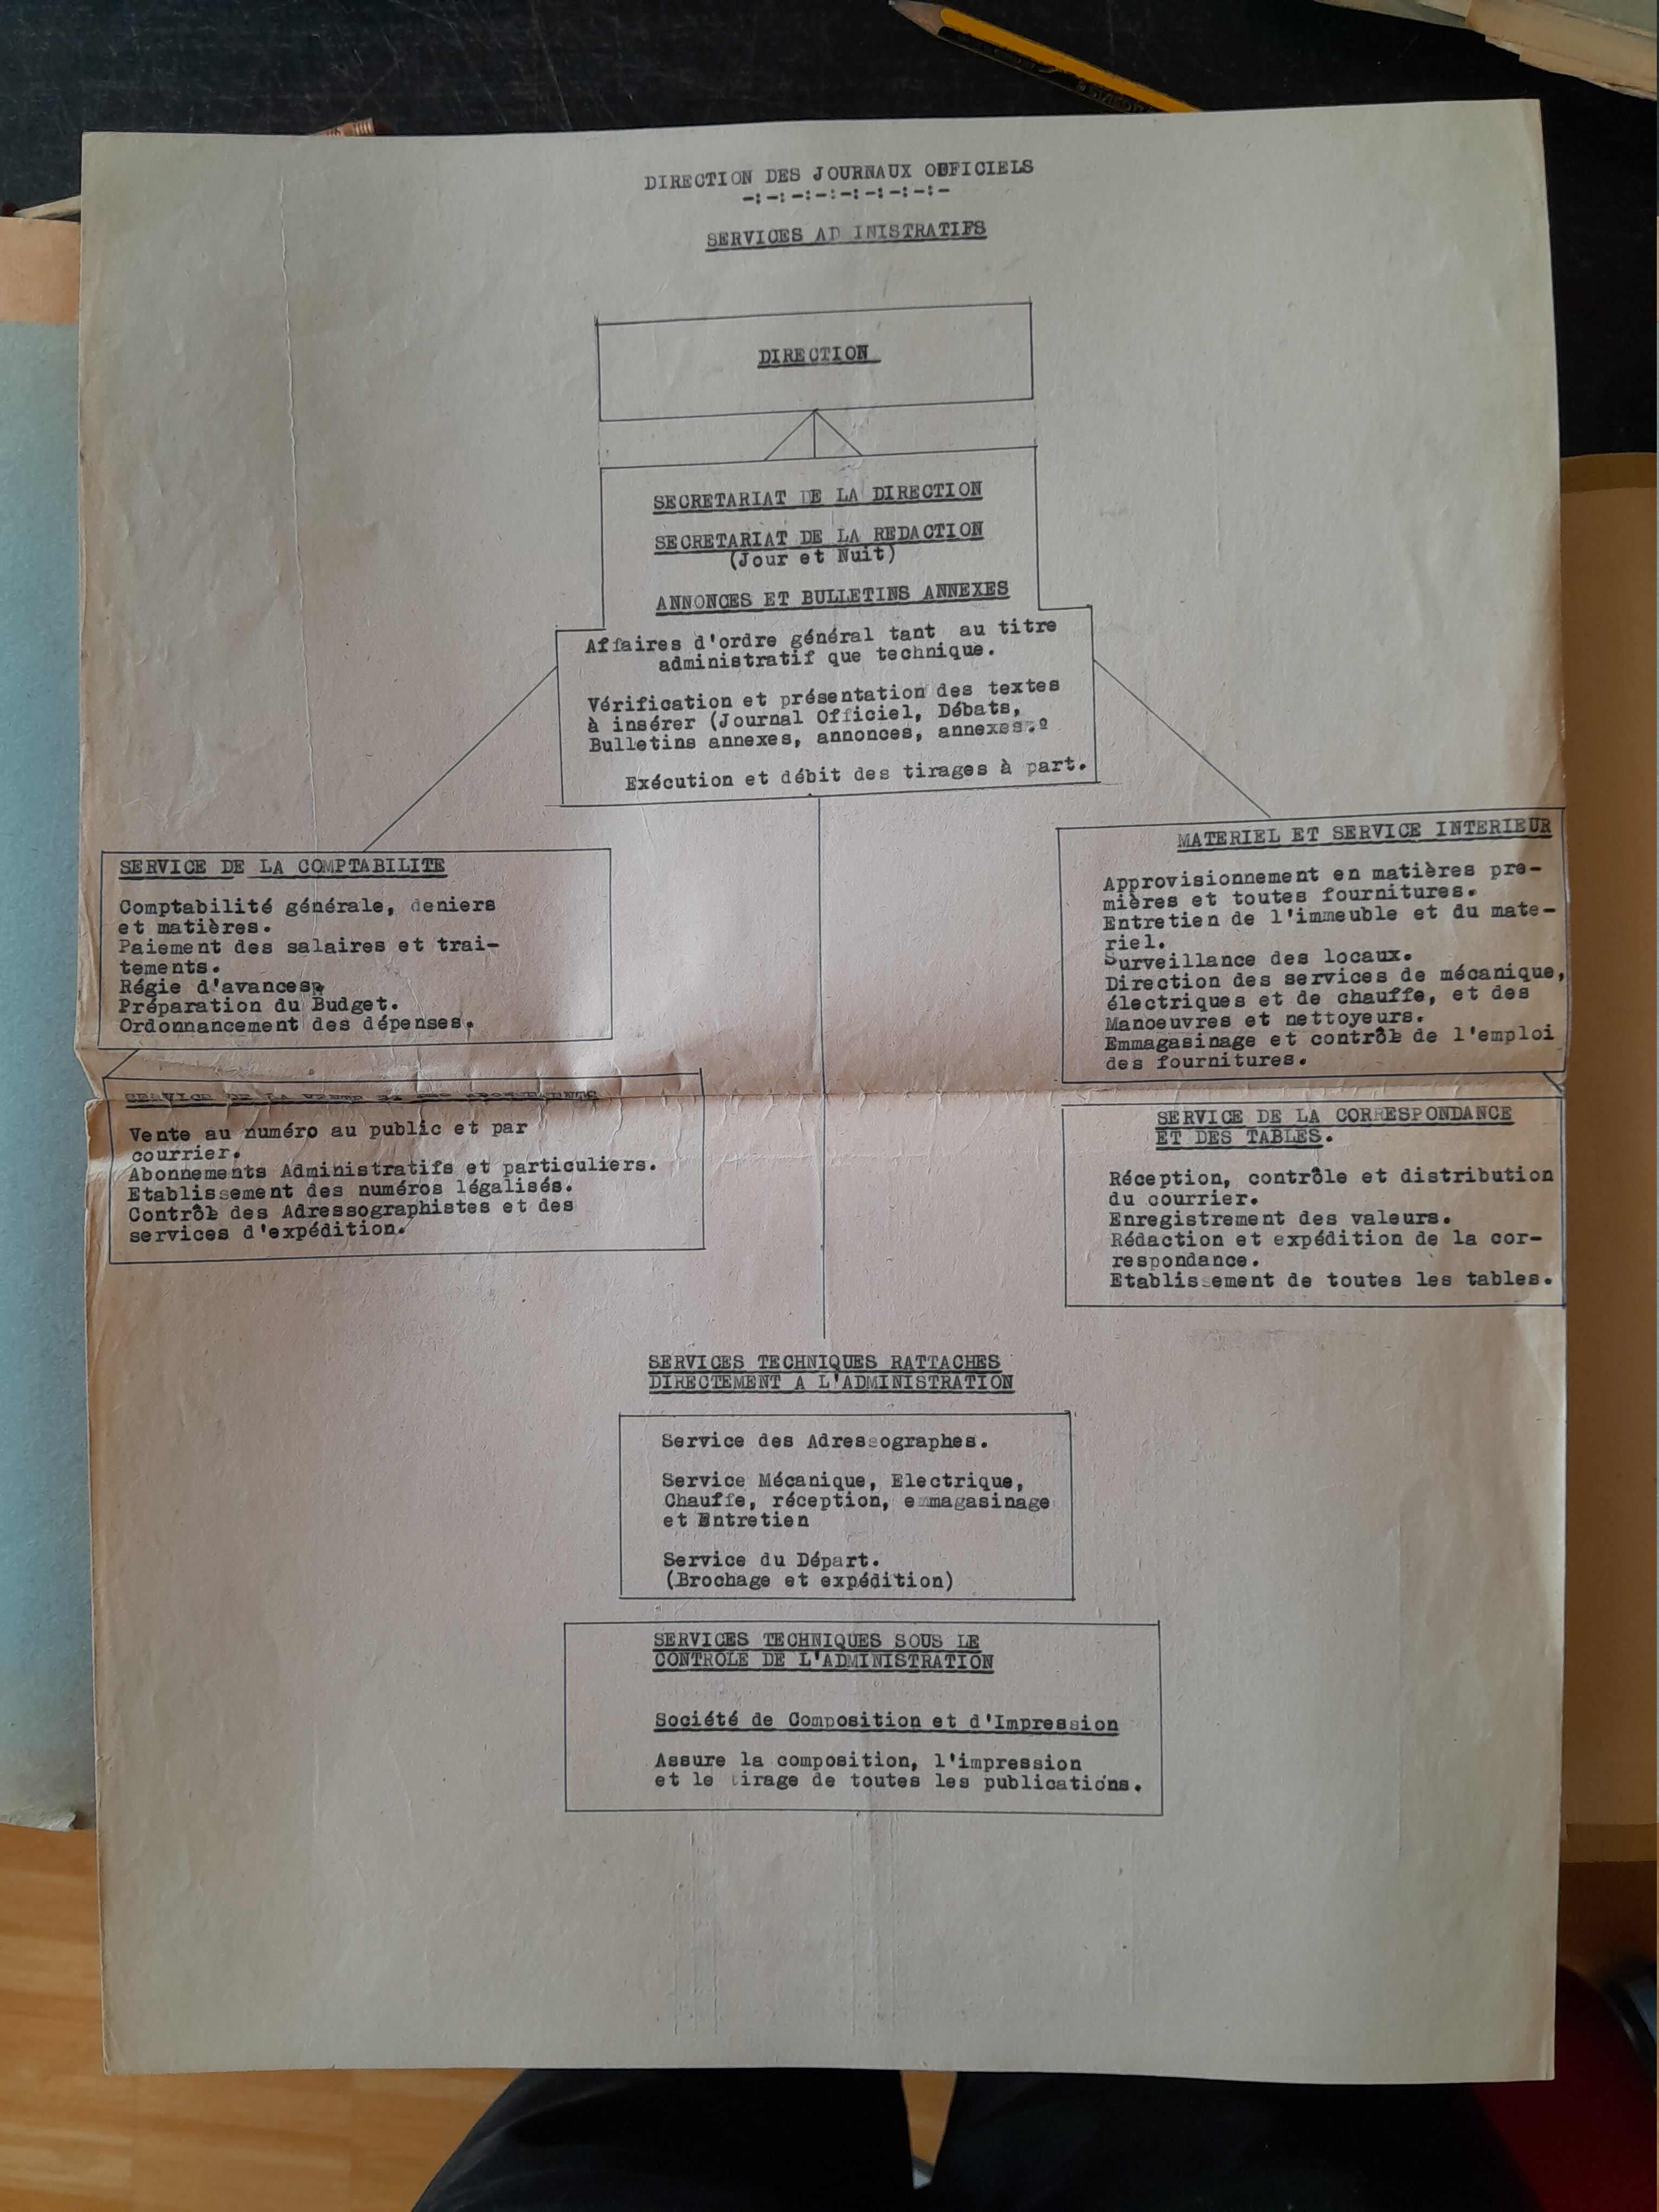
\includegraphics[width=\linewidth]{organigramme.jpg}
\caption{Archives nationales (site de Pierrefitte-sur-Seine), fonds du ministère de l'Intérieur, 19870069/6, Dossier \enquote{Organigramme et personnele} }
\label{fig:organigramme}
\end{figure}

Quant aux \emph{Tables}, elles impliquent un service propre qui a \enquote{un travail minitieux} et \enquote{l'établissement rationnel} d'un système de classement comptant près de 25000 fiches\footcite[][]{cote6}. Le service, en charge de la réalisation des tables alphabétiques mensuelles, des tables des tirages financiers, des Débats de l'Assemblée, des Documents administratifs, des questions écrites et des tables chronologiques, participe également à la lecture et la révision des épreuves. 

On le voit : entre la parole de l'orateur et la lettre imprimée, il y a tout un cheminement documentaire et technique qui implique des choix éditoriaux : quand on travaille sur une telle matière, il faut avoir en tête que ces textes sont le produit d'une chaîne technique assurés par des opérateurs de spécialités très diverses.

\section{Une histoire du \emph{Journal Officiel} par sa nature documentaire : archives ou documentation ?}

Le \emph{Journal Officiel} est une véritable entreprise éditoriale; elle exige une véritable organisation et division du travail pour restituer l'activité parlementaire. Il s’agit maintenant d’interroger sa place dans les dispositifs documentaires et archivistiques car, s'il est soumis au dépôt légal -- il est conservé à la Bibliothèque nationale de France, aux bibliothèques de l’Assemblée nationale et du Sénat, et dans les bibliothèques des Archives nationales. Cette logique de diffusion correspondrait à sa vocation première : rendre publique la loi et l’activité parlementaire, garantir leur accessibilité.

Pourtant, le \emph{Journal Officiel} occupe également une place dans les Archives départementales, au sein de la série K (« Lois, ordonnances et arrêtés »), créée en 1841 : \enquote{la série K, consacrée aux recueils des lois et publications officielles, servira de complément, pour les temps modernes, aux recueils d’édits, d’ordonnances, etc., classés dans la première subdivision de la série A}. Cette série, conçue pour rassembler les actes de l’État et les publications officielles postérieures à la Révolution, accueille non seulement les arrêtés préfectoraux, mais aussi des périodiques comme \emph{Le Moniteur universel}, le \emph{Bulletin des lois} -- puis le \emph{Journal Officiel}. Or, ce classement brouille la distinction classique entre archives (documents produits par une activité administrative et conservés comme traces) et documentation -- objets édités, destinés à la lecture publique. S’il semble naturel que des publications officielles se retrouvent en K et qu’elles cohabitent avec les arrêtés — même s’il est  surprenant d’imaginer que des fonds d’archives s’enrichissent via  l’envoi régulier de périodiques dont il ne manquerait que le bulletinage pour se croire en bibliothèque — , il y a quelque autre chose à chercher du côté de l’histoire du consentement politique.

Cette inclusion du \emph{Journal} dans la série K des Archives départementales ne relève en effet pas d’une simple logique de conservation, mais d’un héritage de stratégie délibérée de fixation et de contrôle de la parole étatique. Comme le souligne Frédéric Graber\footcite[][]{graber}, la création du \emph{Bulletin des Lois} sous le Directoire s'explique à travers le problème de l'observation de la loi. La loi peut être votée et promulguée : elle ne peut obliger que si elle peut être connue de tous. Pour qu’elle soit donc connue de tous et oblige chaque citoyen, la \emph{publication} est donc nécessaire. Il faut \emph{rendre public}, c’est-à-dire \emph{confronter} les citoyens au droit. L’obligation exige l’information : "la formalisation de la publication des lois est l’œuvre cumulée des régimes successifs qui […] ont entrepris de limiter le rôle des 
administrations locales dans le processus de publication de la loi. […] La loi peut être rendue obligatoire sans avoir à la montrer effectivement aux citoyens par l’affiche\enquote{\footcite[][]{graber}. En effet, au début de la Révolution les lois étaient publiées via l’affichage -- dont avait la charge les administrations locales -- et par les crieurs publics. Or, cela  offraient aux administrations locales une plus grande agentivité: en  effet, on pouvait \emph{ne pas} afficher ou retarder l’affichage — ce  qui revient à saboter la confrontation des citoyens au droit et donc de son exécution effective — quand ce n’était pas tout simplement des problèmes techniques d’acheminement ou de réalisation des (ré-)impressions sur place. L’administration déconcentrée, sous le Directoire, peut se montrer effrontée. Ou en tout cas pas  toujours coopérative avec le pouvoir central. Si bien que ce genre de problèmes récurrents a conduit à justifier des approches de publication plus centralisées. Un rapport du 28 brumaire an II (novembre 1793) de Billaud-Varenne, dans un contexte anti-fédéraliste où l’on accuse les administrations  départementales de faire de l’obstruction, dénonce }l’interposition des  autorités secondaires". Suite à ce rapport, la Convention adoptera en décembre (plus précisément le 14 frimaire an II), un décret sur le mode de gouvernement provisoire et révolutionnaire : il crée le \emph{Bulletin des lois de la République}, envoyé à chaque commune par la poste. L’importance de l’affichage public, qui n’est pas vraiment remplacé, sera minoré; les marges de manœuvre des administrations départementales également.

La publication du \enquote{certifié conforme} \emph{Bulletin}, imprimé et envoyé depuis Paris ne fait cependant pas tout à fait office de promulgation, ou en tout cas pas à elle seule. Il y a toujours une proclamation orale de la loi dans les communes et la promulgation est dépendante de cette modalité d’information. Le \emph{Bulletin} est une \enquote{notification aux autorités constituées} : elle est donc un document reçu par les administrations pour qu’elles puissent rendre publique le droit — ce sont leurs  prérogatives — et cela sans passer par le discrétionnaire des agents au  niveau départemental. Ici, on a donc un document opérationnel qui ressemble beaucoup à un document d’archives.

Un autre décret va entériner ce mouvement centripète du pouvoir : le décret du 12 vendémiaire an IV qui institue que la loi devient obligatoire dès que le \emph{Bulletin des Lois} est distribué au chef-lieu du département. Est ainsi instauré \enquote{le régime de publication dans lequel nous vivons encore aujourd’hui, dans  lequel la loi est supposée être connue, parce qu’elle est accessible, mais sans avoir été présentée dans l’espace public, que ce soit oralement ou visuellement}\footcite[][]{graber}. L’effectivité du droit change de régime sensible : il n’est plus une affaire de mots exposés aux regards  et aux oreilles des citoyens. Désormais, le mutisme des textes de lois obligera.

Ce n’est que sous la IIIe République que le \emph{Journal Officiel} prendra ce rôle d’adjuvant à la promulgation par la fonction \enquote{publication} qui était alors une attribution du \emph{Bulletin}. Le \emph{Journal Officiel} est donc génétique a ce \enquote{consentement forcé} de la loi qui s’inscrit pleinement dans l’adage \enquote{nul n’est censé ignorer la loi}. Le respect de la loi au niveau du département est justement une prérogative du préfet. On comprend pourquoi  les arrêtés se retrouvent avec les publications officielles et que cet ordre est une strate du centralisme révolutionnaire puis napoléonien. Et c’est ainsi que les archivistes mentionnés par une circulaire de 1874\footcite[][]{circulaire} aient jugé bon de garder ensemble les documents issus de l’activité Révolutionnaire et les publications officielles ; lesquels se retrouvent dans la série K, car ils sont l’expression du même mouvement de mise en œuvre des stratégies de promulgation des lois par l’État centralisé.

Il ne faut cependant pas conclure que le \emph{Journal Officiel} serait l’instrument qui assujettirait la population aux volontés des politiques. Durant la IIIe République par exemple, et plus encore à ses débuts, la vie politique n’est pas structurée en partis politiques mais plutôt en alliances contingentes\footcite[][]{morel}. Elles se font au gré des ralliements, autour des exercices rhétoriques des parlementaires. Le \emph{Journal Officiel} permet non pas seulement de rendre public l’activité institutionnelle, d’achever l’effectuation du droit par sa publication, mais aussi de faire la publicité des opinions. Il joue un rôle démocratique important. A la Révolution, la création du \emph{Moniteur} est d’abord, et avant le \emph{Bulletin des Lois}, une entreprise de publicité des débats.

Le cadre de classement dit peut être bien quelque chose d’un certain \enquote{énoncé} -- pris ici dans son sens foucaldien \footcite[][]{foucault}, peut être celui de l’organisation politique de l’État sinon de la \enquote{gouvernementalité}. Comme l’ambre d’un fossile, couplé au principe du respect des fonds qui lui est contemporain, il a conservé \enquote{l’ordre du discours} de cette configuration du droit inscrivant son effectivité dans un \enquote{partage du sensible}: ce qui rend le droit effectif ce ne sont, non pas par les mots prononcés ou les mots lus, mais la proximité supposée; l’existence de documents réputés connus et disponibles au sein des services départementaux. Alors faut-il bien distinguer l’effet d’un \enquote{énoncé} politique sur la manière d’organiser des mots et des choses; et la fonction démocratique des publications officielles qui, malgré tout, sont héritières d’une demande sociale de mouture républicaine.

\chapter{Les tables annuelles : des relations documentaires}

\section{Les tables dans l’environnement du \emph{Journal Officiel}}

À côté des livraisons quotidiennes du \emph{Journal Officiel}, le dispositif documentaire de la Troisième République produit un ensemble d’outils de repérage et de cumul : index, tables et recueils annuels. Ces tables, organisées par Chambre et par type de document (séances, questions, interventions, lois, décrets, etc.), constituent un instrument de navigation à travers la masse documentaire accumulée. Elles offrent un second niveau de structuration, indispensable à l’exploitation d’un corpus qui, sans cela, serait pratiquement illisible dans son entier.

Dans ce sens, les tables ne sont pas de simples annexes, mais un élément constitutif du \emph{Journal Officiel}. Leur publication témoigne d’une volonté de rendre praticable la lecture sérielle, en transformant un flot continu de débats en une matière consultable a posteriori. Elles permettent aux parlementaires, aux fonctionnaires et aux juristes, mais aussi aux journalistes et au public, de retrouver un débat, une loi ou un orateur dans un ensemble potentiellement infini de pages.

\section{Forme et organisation des tables}

La table annuelle se présente comme un volume imprimé, distinct des numéros quotidiens mais reprenant la même logique typographique de sobriété. La structuration est généralement alphabétique ou thématique, avec des entrées renvoyant à des numéros de séance ou de page du \emph{Journal Officiel}. Ainsi, le chercheur y trouve à la fois :

\begin{itemize}
\item des index de noms (parlementaires, ministres, orateurs) ;
\item des index de matières (projets de lois, sujets débattus, thèmes abordés) ;
\item des références législatives (dates, intitulés, numéros de lois et décrets).

\end{itemize}
Cette composition apparemment simple reflète un travail complexe de collecte et de mise en ordre, qui engage des méthodes d’indexation encore largement manuelles dans les années 1930. Les tables matérialisent donc une double médiation : celle de la transcription sténographique, puis celle de la mise en indexation.

\section{Informations sémantiques et usages}

Les tables ne livrent pas seulement des renvois. Leur organisation alphabétique ou thématique suggère déjà une lecture orientée du corpus. En réordonnant les débats selon les sujets ou les personnes, elles produisent une représentation « secondaire » de l’activité parlementaire :

\begin{itemize}
\item \textbf{Pour l’historien}, elles permettent de cartographier les thèmes récurrents, d’identifier des trajectoires individuelles de parlementaires, ou encore de suivre la maturation d’une question dans le temps long.
\item \textbf{Pour les juristes}, elles assurent un repérage efficace des textes normatifs, condition de la sécurité juridique.
\item \textbf{Pour l’administration}, elles facilitent la réutilisation interne des débats et la circulation de l’information entre services.

\end{itemize}
En ce sens, les tables possèdent une valeur sémantique propre : elles ne sont pas de simples index, mais des instruments de catégorisation, qui hiérarchisent les contenus du \emph{Journal Officiel} et leur confèrent une visibilité inégale.

Les tables comme « hub » intercorpus

Enfin, les tables établissent des liens entre différents ensembles documentaires. Elles ne se limitent pas aux seuls débats parlementaires, mais relient ceux-ci aux autres publications officielles et à des corpus complémentaires. Elles servent d’articulation entre :

\emph{ les volumes quotidiens du }Journal Officiel* ;
\emph{ les recueils législatifs et réglementaires (par exemple le }Bulletin des lois*) ;
\begin{itemize}
\item les instruments internes des Chambres (procès-verbaux, rapports de commissions) ;
\item les archives départementales (série K), où elles prennent place aux côtés d’autres formes de publicité administrative.

\end{itemize}
En occupant cette position nodale, les tables fonctionnent comme des « hubs documentaires » : elles permettent de passer d’un corpus à l’autre, et d’inscrire les débats dans l’écosystème plus large des pratiques de gouvernement.

Exemple : Les Tables du Sénat, année 1931

Le volume des \emph{Tables annuelles du Sénat} pour l’année 1931 se présente sous la forme d’un in-octavo relié, composé de plusieurs centaines de pages. La typographie, sobre et régulière, reprend les conventions du \emph{Journal Officiel} : colonnes étroites, numérotation continue, absence d’ornementation. L’ensemble se divise en sections distinctes, qui reflètent les usages concrets des lecteurs.

\subsection{Index des orateurs}

On y trouve une \textbf{liste alphabétique des sénateurs}, chaque nom suivi de références aux séances où ils sont intervenus. Par exemple :

\begin{quote}
\emph{Tardieu (André)} : interventions p. 312, 457, 892.

\end{quote}
Cet index permet de retracer rapidement la présence et l’activité d’un parlementaire sur une année complète. Pour l’historien, il offre une base sérielle pour mesurer la visibilité des élus et la fréquence de leur participation aux débats.

\subsection{Table des matières thématiques}

La deuxième section regroupe les débats par \textbf{matières} :

\emph{ }Finances publiques* : budget, impôts, emprunts.
\emph{ }Affaires étrangères* : traités, conventions, mandats.
\emph{ }Travail et questions sociales* : assurance chômage, législation ouvrière, retraites.

Chaque entrée renvoie à un numéro de séance du \emph{Journal Officiel}. Ce classement thématique reflète une logique documentaire propre, qui diffère de l’ordre chronologique des séances : il met en valeur la récurrence des thèmes et facilite leur repérage transversal.

\subsection{Références législatives et réglementaires}

Enfin, les tables recensent les \textbf{lois votées et les décrets publiés} pendant l’année, assortis de leur date et de leur numéro. Ce registre, proche d’un répertoire législatif, assure le lien avec le \emph{Bulletin des lois} et, par extension, avec l’ensemble de la législation nationale.

 Analyse

Cet exemple illustre trois dimensions essentielles des tables :

\begin{itemize}
\item Leur \textbf{fonction instrumentale} : elles servent avant tout de guide, destiné à faciliter la recherche d’une information précise dans un corpus immense.
\item Leur \textbf{valeur sémantique} : en proposant une catégorisation (par personnes, thèmes, textes), elles produisent une image de l’activité parlementaire qui n’est pas neutre, mais orientée par le mode d’indexation.
\item Leur \textbf{rôle intercorpus} : en mettant en relation débats, interventions et textes normatifs, elles constituent un point de jonction entre la parole parlementaire et le droit promulgué.
\end{itemize}





%%%%%%%%%%% PARTIE 2
\part{L'enjeu des données structurées : des sources à la base de données}


\chapter{Une histoire par les données}

Les \emph{Tables Annuelles} du Sénat, comme on vient de le voir, contiennent une véritable mine d'informations pour établir une analyse de l'activité parlementaire. Ces \emph{Tables}, accessibles sur Gallica, avec le jeu des renvois et des index, sont de véritables bases de données de papier numérisées. Pour récupérer les informations du \emph{Journal Officiel} de façon automatisée, c'est-à-dire sans reproduire à la main l'ensemble, il faut penser à une chaîne de traitement qui part de ces sources numériques, sous format image, pour pouvoir en capturer l'information. Il s'agit ici de voir comment construire un protocole d’extraction cohérent, en tenant compte de la matérialité des documents eux-mêmes, aussi bien sous leur forme \enquote{analogique} que numérique. 

Dans ce chapitre, il s'agira de répondre aux problématiques technique de cette traduction des sources numérisées -- c'est-à-dire sous format image -- au texte. Ceci imposant de donner un contexte préalable de cette \enquote{mise en données}\footcite[][]{clavert} des sources historiques, laquelle est inhérente à la disponibilité de corpus numérisés par les politiques de valorisation des fonds des institutions patrimoniales. [Section 1: Datafication des corpus : \enquote{numériser}]

Ensuite, premier problème : comment travailler à partir d'une image numérique ? Certes, la représentation photographique et numérique d'un document est lisible pour un oeil humain; mais du point de vue informationnel, ces images ne sont que des paquets de pixels, une conversion numérique de l'information lumineuse renvoyée par les objets photographiés\footcite[][]{claerr}. Ces pixels ne sont pas, évidemment, les lettres elles-mêmes. Ils sont la traduction sur l'écran de trains d'informations binaires qui, sans le bon décodage, pourrait vouloir dire tout autre chose. Le premier enjeu pour un travail de capture de l'information est de transformer cette matière matricielle en information textuelle sur laquelle on peut appliquer des traitements. Le texte se présente comme pré-requis pour établir des chaînes de traitement de capture informationnelle. Ce passage de l'image au texte numérique est en fait techniquement une prérogative des tâches de \emph{reconnaissance optique des caractères} -- ou \enquote{OCR} (Optical Character Recognition). Elle butte également sur des problématiques de détection de la mise en page, laquelle fonde un ordre de lecture -- et donc un agencement du sens des phrases qu'il faut considérer. [Section 2 : de l'image au texte]

Deuxième problème : une fois ce texte numérique obtenu, comment capturer l'information sémantique qui est présente ? Comment l'ordinateur peut comprendre que tel ensemble des caractères alphanumériques correspond en fait à un sénateur de la Troisième République ? On peut trouver, dans le document, des motifs qui signalent une entité (par exemple, un sénateur inaugure chaque paragraphe). Cette approche comme on va le voir, est basée sur la reconnaissance de motifs typographiques. Elle est cependant fragile et dépendante de la qualité de l'OCR -- voire des erreurs humaines présentes dans le document d'origine. Elle suppose aussi une forme de connaissance \emph{a priori} synthétique de la représentation de l'information dans le document. Ainsi peut-on se tourner vers des approches extractives qui viennent labelliser l'information textuelle obtenue\footcite[][]{finkel}; ou bien les approches génératives qui \enquote{lisent} le texte et restituent l'information comprise et permettent de contourner le problème des exceptions qui forment le corps des documents\footcite[][]{radford}. Cette chaîne de travail de capture exige une information exploitable par l'ordinateur; elle a besoin d'une certaine systémacité, laquelle est une prérogative des modèles de données -- de leur \enquote{forme}. La chaîne de traitement commence donc avec l'image, passe par le texte et des méthodes de capture de l'information sémantique qu'elle contient, pour aboutir à une information structurée. L'enjeu n'est pas simple car chaque étape reporte les marges d'erreur des précédentes. [Section 3]

Dans ce chapitre, il s'agira ainsi de dessiner le contexte technique et institutionnel de cette datafication des données en vue de leur traitement -- et notamment avec les nouvelles opportunités des grands modèles de langage.

\section{Numériser les sources}

\subsection{En \enquote{mode texte}}

En 1971, un étudiant, reproduisait sur un ordinateur \emph{Xerox} la \emph{Déclaration d'indépendance des Etats-Unis}, en caractères alphanumériques \textbf{ASCII}. Il s'agissait de Michel Hart, fondateur du \textbf{Projet Gutenberg} qui se donnait pour tâche de reproduire et diffuser bénévolement sur le réseau internet des oeuvres littéraires du domaine public. Des livres comme \emph{La Bible}, des oeuvres de Shakespeare, quelques autres de Lewis Carroll ou de James M. Barrie seront notamment reproduites \footcite[][]{lebert}. Ce travail de \enquote{numérisation} est en fait un travail laborieux, sinon de tâcheron : chacune des lettres de chaque livre sera tapée à la main, les unes après les autres. En 1990, de façon contemporaine à la jeunesse du Web, le projet prend un nouvel essor et bénéficie d'une collaboration internationale : les collections s'élèvent à environ 1000 livres en 1997; 4000 livres en 2001; et $15000$ livres en 2005 \footcite[][]{lebert}. Entre le livre et la version numérique, il n'y a pas d'image : juste le travail de transcription manuel des caractères. C'est une numérisation des livres \enquote{en mode texte} \footcite[][30-33]{bermesbook} : l'information textuelle seule, stockée sur disque dur, est reproduite sur l'écran, cela \enquote{destructurant l'objet livre} \footcite[][]{bermesbook}. Avec cette reproduction en caractères alphanumériques, la structure physique du livre -- sa mise en page -- est perdue; mais on peut en revanche rechercher un mot et retrouver un passage plus aisément. 

Le texte numérique ne se définit pas seulement comme une reproduction électronique du texte imprimé, mais comme une transformation de l’information en une suite de signes codés. Concrètement, chaque caractère est représenté par une valeur numérique, selon un système de codage -- ainsi tel que l’\textbf{ASCII} (American Standard Code for Information Interchange) ou, plus récemment, l’\textbf{Unicode}, qui attribue à chaque lettre, chiffre ou symbole une séquence binaire, une suite de \emph{bits}, c’est-à-dire de 0 et de 1. Ce passage de l’écriture alphabétique à la codification binaire permet au texte d’être manipulé comme une donnée discrète : il devient possible de rechercher automatiquement un mot, de compter des occurrences, de structurer des chaînes de caractères.

Cette démarche d'encodage de l'information, qui ne concerne pas ici proprement l’historien, est exemplaire au regard des méthodes de \emph{numérisation} des documents textuels en ce sens qu’elle traduit une forme analogique — physique ou continue — en une forme numérique, discrète. L’opération de transcription manuelle, caractère par caractère, est ici comparable à celle d’un dépouillement systématique sur archives papier : il s’agit de saisir l’information contenue dans les sources dans un dispositif tabulaire, par exemple un tableur \footcite[][]{zalc}. La similarité n’est toutefois que d’ordre opératoire. Même si les enjeux intellectuels ne sont pas les mêmes, il y a un face-à-face entre un opérateur et la source à restranscrire. Il y a une reproduction qui n'est pas photographique, mais manuelle. Dans le cas de Michel Hart et du Projet Gutenberg, la répétition du texte littéraire reste relativement linéaire et vise une reproduction intégrale. À l’inverse, la transcription historienne -- qui n'est pas nécessairement moins laborieuse -- suppose \emph{en même temps} une enquête critique : sélectionner, structurer, et souvent synthétiser des données pour les « mettre en table », c’est-à-dire les rendre comparables, quantifiables. La transcription de sources historiques est tournée vers sa structuration, d'une \enquote{mise en fiche}\footcite[][]{bertfiche}, même si celle-ci est implicite -- par exemple l'ordre des éléments transcrit est une information séquentielle de cheminement de lecture. Ce schème opératoire transcriptif peut être qualifié, avec Simondon, de travail de \emph{transduction}\footcite[][p. 76]{chatonsky} : un processus par lequel l’information passe d’un support et d’un régime de signification à un autre, selon des contraintes à la fois techniques et des exigences intellectuelles. Dans le cas de la transcription numérique, l'information change de milieu technique et son inscription \emph{in silicium} permet de reconsidérer le texte discrétisé comme un ensemble d'éléments manipulables, par exemple par des algorithmes de tri. Le texte numérique peut être alors considéré selon différents degrés de structuration : tantôt comme une \enquote{répétition linéaire} et brute des sources originales à l'instar des premières éditions du \textbf{Projet Gutenberg}; tantôt comme une information choisie et hiérarchisée, tendue vers un raffinement structurel, comme l'implique une mise en tableau.

Dans le cas des historiens, ce passage implique un véritable travail d’individuation des données -- c'est-à-dire de leur transformation au regard du contexte technique qui joue ici comme un milieu : il faut découper des flux documentaires continus en unités discrètes (noms, dates, professions, événements par exemple), qui ne préexistent pas à l’opération de transcription mais sont construites, reformulée par elle, avec la contrainte ultérieure de pouvoir retrouver l'information encodée. Des stratégies d'habillage de l'information saisie sont à envisager du même mouvement, par exemple en dotant le texte d'un \enquote{apparat critique} qui permettent un retour au texte original à travers des clés qui en indexe le contenu \footcite[][]{vancampenhoudt}. La numérisation en mode texte est alors une opération configuratrice : la saisie manuelle se fait l’instrument d’un changement de régime technique du support de l'information car elle implique, à différent degrés, un besoin de mise en structure. Du côté des historiens, si ce travail de transduction informationnelle, plus sophistiqué que la transcription littérale, peut être comparé au travail de terrain du sociologue ou de l'éthnographe -- en ce sens qu'elle suscite justement des questions et reconfigure les valuations de l'enquête \footcite[][]{zalc}\footcite[][]{dewey} -- il s'adosse surtout à l'élaboration de nouvelles données sur les données collectées. Ces \enquote{données sur les données} -- ces \textbf{métadonnées} --, nécessaires par exemple pour mettre en table l'information obtenue, relèveraient d'un \emph{design} ou, autrement dit, d'une stratégie de composition de l'information en vue d'en produire une représentation intellegible pour un traitement ultérieur\footcite[][]{renon}. Ces métadonnées, plus ou moins riches ou explicites mais qui permettent de ranger les données collectées, sont propre à l'historien qui ajuste ces catégories à ses besoins. Si bien que ce processus valuatif de mise en catégorie de l'information capturée accompagne la transcription manuelle et littérale des sources. Elle s'inscrit dans une démarche éditoriale telle que décrite par Steven DeRose, David Durand, Elli Mylonas et Allen Renear, qui se représentent le texte comme une structure hiérarchique ordonnée d'objets et de contenu \footcite[][]{derose}. 

Le travail de saisie manuelle, avec ou sans métadonnées, n’est évidemment pas une nouveauté introduite par l’ordinateur. Bien avant l’ère numérique, les historiens s’y adonnaient déjà. Ainsi, Pierre Chaunu qui, en 1947, recopiait à la main, sur papier, les données issues des archives microfilmées et des ouvrages nécessaires à sa thèse, afin de les ordonner et de les exploiter systématiquement \footcite[][]{muller}; ou encore Ladurie sous forme de fiches ou de tableaux [Ladurie]. Au-delà du \enquote{bricolage} \footcite[][]{levi-strauss} transcriptif, propre à chaque chercheur, l'histoire de la fiche érudite nous indique également des ambitions de systématisation lesquelles conduisent à une véritable ingénierie du glanage documentaire \footcite[][]{bert}. Citons par exemple \enquote{l'armoire érudite}, les boîtes ou les casiers extensibles de l'entreprise \emph{Borgeaud} permettant de ranger l'information dans des bonnes cases, le casier où la position dans un classeur ayant valeur ici de \enquote{métadonnée analogique}\footcite[][]{bert}. Aujourd’hui encore, malgré l’apparition d’outils de transcription automatique [voir section 2], cette pratique demeure courante : toutes les sources ne sont pas disponibles en version numérique, et le chercheur, tout comme l’étudiant ou le généalogiste, peut être amené à relever lui-même les informations qui l’intéressent, directement en salle d’archives ou lors du dépouillement de fonds imprimés. 

Le mode opératoire de la numérisation « en mode texte » constitue en ce sens un cas exemplaire, puisqu’il s’oppose radicalement à la logique de la numérisation photographique, dite « en mode image » \footcite[][]{bermesbook}\footcite[][]{claerr}. Il ouvre également des perspectives pour le traitement quantitatif, dans la mesure où il produit une matière directement exploitable : des données susceptibles d’être structurées — par une mise en table ou un encodage hiérarchique tel que la \textbf{TEI} — et manipulées — par exemple à travers la recherche de motifs textuels.

\subsection{En \enquote{mode image}}

À l’opposé du « mode texte », la numérisation en \enquote{mode image} repose sur la reproduction photographique des documents, cherchant à restituer leur matérialité visuelle : texte, blancs, marges, typographie, ornements, etc. Tout est fixé dans une matrice de pixels. Héritière des microfilms et des fac-similés, cette pratique connaît une expansion décisive dans les années 1990, avec l’essor du Web et le lancement des premières grandes campagnes institutionnelles de numérisation. Deux projets emblématiques illustrent cette dynamique : Gallica (BnF, 1997) et Google Books (2004)\footcite[][]{bermesbook}. Leur ambition est similaire — mettre à disposition le patrimoine imprimé à grande échelle — même si, pour Gallica, il s'agit de s’inscrire dans une mission de service public. Dans les deux cas, la numérisation institutionnelle en mode image suppose des investissements lourds en infrastructures, en personnels et en politiques documentaires\footcite[][p. 66-88]{claerr}. Elle se distingue ainsi des pratiques de transcription textuelle, souvent issues de gestes individuels ou collaboratifs (historien recopiant ses sources, dépouillements collectifs, corrections d’OCR par \textbf{crowdsourcing}). Certes, des chercheurs ou amateurs produisent eux aussi des photographies de documents — parfois propres, parfois très imparfaites —, mais ces fichiers, à défaut d'un soin documentaire, restent isolés, de qualité variable, sans métadonnées ni garantie de pérennité. Si bien qu'ici, photographier soi-même ses sources -- par exemple aux archives -- ne revient finalement qu'à remettre à plus tard le travail de dépouillement. Ce qui d'ailleurs n'empêche finalement une laborieuse transcription en mode texte mais non plus en face des sources mais de leur reproduction numérique. 

Sur le plan technique, ces images sont matricielles : elles fixent l’apparence de la page mais le contenu intellectuel \enquote{littéraire} demeure opaques pour l’ordinateur. Une image numérique est un tableau -- une \emph{matrice} -- d'une largeur et d'une hauteur données, comportant alors largeur $\times$ hauteur pixels, pixels qui encode l'information colorimétrique sur trois vecteurs : le paramètre $rouge$, le paramètre $vert$, et le paramètre $bleu$. La combinaison de ces trois paramètres, selon les règles de la synthèse colorimétrique additive, permettent de restituer, pour chaque pixel, l'ensemble des couleurs du spectre visible. Qu’elles proviennent d’une campagne institutionnelle ou d’un smartphone amateur, elles ne permettent pas la recherche plein texte sans OCR ou segmentation. Dans le cas des photographies amateurs, pouvant être floues ou mal cadrées, l’OCR est même impraticable, réduisant ces fichiers à des fac-similés inertes, reportant ainsi la tâche de saisie manuelle non pas à partir des documents matériels, mais à partir de leur représentation numérique. Ce qui permet de souligner que ce n'est pas la technique de numérisation qui \enquote{fait} le mode opératoire; mais bien le rapport de l'opérateur à un système technique plus ou moins sensible à l'information et sa capacité à la transformer\footcite[][]{meot}.

En effet, \enquote{numériser n’est pas éditer} \footcite[][]{bermesblog}. Là où la mise en table implique un travail de curation plus ou moins entendu — sélection, structuration, annotation —, la capture photographique ne livre qu’une matière brute. Sans enrichissement éditorial, sans métadonnées ni transcription automatique, ces images demeurent orphelines de leur contenu textuel : de simples objets visuels, inaccessibles à toute interrogation systématique. Leur valeur scientifique dépend donc entièrement des traitements ultérieurs qui les convertissent en données exploitables. Dans le cas de la numérisation amateur, ces fichiers constituent le plus souvent un point de départ, ou une stratégie mnémonique pour différer le travail de transcription lors de l’enquête sur les sources. À l’inverse, pour la numérisation institutionnelle, ils relèvent d’une logique patrimoniale : il s’agit avant tout de restituer des ouvrages de nature variée par la reproduction photographique, solution pragmatique mais qui pose d’emblée la question de l’alternative avec le mode texte. Comme le rappelait Jean-Didier Wagneur à propos de Gallica :

\begin{quote}
« Nous avions le devoir patrimonial de restituer l’image du document tel qu’il a été déposé et le choix du mode image (fac-similé électronique) s’est imposé. Cette option a été à l’origine de nombreuses questions autour de l’alternative que le mode texte présentait. […] On voit qu’à terme, la saisie en mode texte aurait débouché sur la nécessité de produire des documents mixtes (texte et image) afin de préserver l’intégrité de tous les documents de nature graphique (illustrations, cartes, reproductions, graphes et expériences scientifiques) figurant dans les ouvrages numérisés. » \footcite[][]{wagneur}

\end{quote}
Se dessine une tension durable entre deux régimes de numérisation : d’un côté, la transcription textuelle qui repose sur la couteuse \enquote{nécessité de faire saisir les œuvres de plusieurs centaines, voire milliers, d’auteurs} exigeant un \enquote{accompagnement scientifique considérable}\footcite[][]{wagneur}; de l’autre, la reproduction visuelle, portée par des politiques institutionnelles, qui fabrique des corpus massifs mais souvent réduits à l’état de matière brute.

\subsection{La \enquote{datafication}}

Cette opposition doit enfin être replacée dans l’horizon plus large de la \emph{datafication}\footcite[][]{clavert}. La \emph{datafication} est le processus qui vise à quantifier un phénomène de sorte qu'il soit calculable et analysable \footcite[][]{clavert}. Elle est en quelque sorte un \enquote{schème opératoire} \footcite[][p. 236]{meot} permettant la calculabilité des sources avec un outillage informatique. Cette mise en données \enquote{insiste sur la notion de processus} et \enquote{se définit par les choix opérés par les organismes qui y procèdent}, cela impliquant \enquote{les critères d'inclusion [de] corpus à numériser}; l'élaboration de métadonnées descriptives situées, lesquelles ont un impact sur leur découvrabilité puisque les moteurs de recherche s'y appuient \footcite[][p. 123]{clavert}.

Si bien que numériser, ce n’est pas seulement reproduire. C’est transformer des artefacts en données, dans un cadre technique, social et institutionnel qui oriente les usages, fixe les normes de conservation et conditionne l’accès même aux sources. Elle met en évidence deux conceptions distinctes de la numérisation: d’un côté, la transcription textuelle, qui construit les données par un travail de sélection et est tendue vers une structuration plus ou moins affirmée; de l’autre, la reproduction visuelle, qui se limite à conserver une représentation plane de la matérialité de l’objet. L’histoire des pratiques documentaires de \enquote{mise en données} témoigne de cette tension durable entre deux paradigmes concurrents \footcite[][p. 29]{bermesbook} qui sont alors autant techniques qu'institutionnels. En suivant Bruno Latour, on peut dire que \enquote{nous ne devrions jamais parler de ‘données’, mais toujours d'‘obtenues’} \footcite[][]{goeta}. La saisie manuelle n'est pas une simple transplantation de contenu, mais une construction — un fait mobilisable conditionné par des choix de catégorisation, de format, et d’usage. La reproduction photographique, à l’inverse, ne produit pas directement de données exploitables, mais fige l’apparence visuelle du document, laissant le texte dans un état opaque tant qu’aucune opération d’extraction ou d’annotation n’est réalisée. 

Chaque \enquote{mise en données} est ainsi moins une instanciation pure de la source dans le giron du binaire qu'une stratégie épistémique de sa présentation au sein d’un réseau sociotechnique instituant \footcite[][]{renon}. Dans cette perspective, on peut dire avec Cornelius Castoriadis que la numérisation est un geste \enquote{instituant} : elle crée de nouvelles manières de faire exister et de rendre visibles les sources, conditionnant les régimes d’intelligibilité qui en découlent\footcite[][]{rautenberg}. Or, au sein des politiques contemporaines de numérisation, cette dimension instituante prend une forme discursive et normative particulière : celle du \emph{patrimonial}. Le patrimoine est un « passé-présent » sans cesse réinterprété, qui puise dans l’imaginaire institué et reforme en retour de nouvelles significations. La numérisation est justifiée et orientée par un vocabulaire de démocratisation et de valorisation, dans une fibre tout encyclopédique, tel que défendu par Jean-Didier Wagneur cité précédemment. Autrement dit, ce qui est numérisé n’est pas seulement conservé ou reproduit : il est institué comme patrimoine, doté d’une valeur \enquote{émotionnelle} et sociale spécifique \footcite[][]{bermesbook}. Les données produites par la numérisation sont donc indissociables d’une politique culturelle qui configure les conditions d’accès, de visibilité et de réutilisation des corpus, ce qui implique nécessairement des biais de sélection ou tout simplement des priorités déterminées par les politiques de conservation de documents fragiles.

\subsection{Pratiques historiennes : sphère technique, sphère sociale}

La datafication ne consiste donc pas seulement en un enchaînement d’opérations techniques — OCR, structuration, encodage —, mais en un processus situé, au croisement de la sphère technique et de la sphère sociale. Il n’existe pas de \enquote{données brutes} : toute donnée est déjà une \emph{capta}, c’est-à-dire une information \enquote{prise}, construite dans et par un cadre interprétatif qui reflète des choix méthodologiques et institutionnels \footcite[][]{drucker}. Leur mise à disposition est elle-même également une affaire de visualisation : la mise en ordre des résultats d'une recherche en ligne appartient au giron de la visualisation des données -- et comme on l'a sous entendu précédemment, les stratégies épistémiques de représentation de connaissance est une affaire de \emph{design}. D'ailleurs certains artistes comme le duo Vasulka, dans la même veine du concept de \emph{graphesis} de Johanna Drucker \footcite[][]{drucker} parlent volontiers de \enquote{nouvel espace épistémique}, \enquote{d'\emph{épistémè numérique}}\footcite[][]{dallet} ou encore \enquote{d'image relation} \footcite[][]{boissier}, ce dernier concept insistant plutôt sur la notion d'interactivité. Pour ces artistes, il est question de faire grincer la dimension interprétative et graphique de l'accès à l'information à travers des interfaces car, si l'habitude peut nous conduire à considérer la présentation des données par des moteurs de recherche comme \enquote{objectifs}, il faut au contraire montrer qu'il s'agit de dispositifs techniques partiaux, construit historiquement \footcite[][]{daston}. S'il peut bien y avoir une prétention encyclopédique dans les dispositifs techniques d'accès aux sources \footcite[][]{wagneur}, il y a également une dimension esthétique, \enquote{jouable}, qui est une condition à la lisibilité du dispositif numérique\footcite[][]{boissier}. Dès lors, il faut considérer les données et les métadonnées à la lumière de leur présentation, présentation qui doit faire l'objet de décisions, de stratégies au regard de ce qui importe de montrer ou de cacher -- bref : il y a là des \emph{valuations} dans la médialité, en reprenant ce mot dans son sens deweyien\footcite[][]{dewey}, c'est-à-dire une dépendance des schèmes techniques opératoires aux processus de formation des valeurs. Les institutions patrimoniales sont des acteurs exemplaires de cette double dépendance des dispositifs techniques aux attentes sociales ou scientifiques. Un exemple particulièrement riche de ces réflexions se trouve dans le PLAO (pour \enquote{Poste de Lecture Assistée par Ordinateur}) imaginé à la BnF dans les années 1990 sous l’impulsion de Bernard Stiegler. Il s’agissait d’une interface destinée à incarner le lecteur « savant » au cœur d’un dispositif instrumenté, permettant non seulement de consulter des textes numérisés, mais aussi de les annoter, de structurer dynamiquement un corpus, de naviguer, d’archiver, de copier ou d’indexer en temps réel. Le PLAO n’est jamais devenu un équipement déployé à large échelle, mais il s’est imposé comme un \enquote{objet-frontière} — au sens de Star et Griesemer — structurant une coalition entre informaticiens, philosophes, historiens et bibliothécaires, engagés dans la conceptualisation d’un nouvel usage de la bibliothèque numérique\footcite[][]{bequet}.

Ces interrogations contemporaines ne surgissent pas \emph{ex-nihilo}: elles prolongent une histoire plus ancienne des rapports entre historiens et outils informatiques. Ces transformations récentes s’inscrivent dans une histoire plus longue des usages de l’informatique par les historiens. Dès les années 1950, des expériences pionnières lient mécanographie et analyse sérielle \footcite[][]{daumard}, dans la lignée des « archives quantitatives » chères à l’école des \emph{Annales}. Dans les décennies 1960–1970 voient s’imposer l’ambition d’une histoire totale \footcite[][]{poublanc}. La prophétie de Le Roy Ladurie — « l’historien de demain sera programmeur ou ne sera pas » — illustre cet horizon, même si les limites de l’histoire sérielle conduisent rapidement à relativiser l’objectivité promise par la machine. Dans les années 1980–1990, l’apparition du micro-ordinateur personnel, puis des premières bases de données relationnelles et de revues comme \emph{Le Médiéviste et l’Ordinateur}, favorise une technicisation diffuse des pratiques, souvent portée par des chercheurs passionnés plutôt que par une politique disciplinaire globale \footcite[][]{poublanc}. Le Web, à partir de la fin des années 1990, change l’échelle de ces usages : il facilite l’accès et la diffusion des corpus (Gallica, revues.org) et transforme le rapport aux archives grâce aux appareils photo numériques et aux interfaces de recherche. L’émergence des humanités numériques dans les années 2000 fait de ces pratiques dispersées un champ identifié, mais aussi un espace de tensions : entre injonctions institutionnelles, résistances disciplinaires et négociations interdisciplinaires. L’histoire des pratiques historiennes « numériques » apparaît ainsi comme un processus long, fait d’allers-retours entre engouements, critiques et réinventions, qui relativise l’idée d’un tournant soudain pour insister sur la continuité d’une adaptation progressive des historiens à leurs outils.

Avec l’essor du Web, la datafication ne se réduit plus à un geste de transcription ou à un choix institutionnel de numérisation : elle s’inscrit dans des infrastructures réticulaires qui conditionnent la circulation et l’usage des corpus. Les documents ne sont pas seulement mis en ligne ; ils sont exposés à travers des protocoles techniques — comme les API — qui déterminent la granularité d’accès, la possibilité de réutilisation et la manière dont les sources sont découvertes. Comme le montre l’exemple du \emph{Goût de l’archive à l’ère numérique} et de sa réflexion sur le \enquote{goût de l’API}\footcite[][]{goutapi}, l’archive numérisée devient un objet relationnel : elle n’existe pleinement qu’à travers les réseaux qui l’indexent, la connectent et la rendent interopérable avec d’autres ensembles de données. Cette dimension réticulaire transforme profondément la sphère sociale des archives : les corpus ne sont plus simplement conservés et transmis, mais distribués, exposés, parfois fragmentés, selon des logiques de plateformes et de moteurs de recherche. La découvrabilité des sources dépend ainsi de ces dispositifs techniques saisis dans des processus de concrétisation [Simondon], qui agissent comme de nouveaux médiateurs documentaires et configurent, en amont, les conditions de possibilité de l’enquête historienne. 

Autrement dit, ce que fait la numérisation aux corpus, c’est moins de les rendre \enquote{disponibles} que de les reconfigurer: par la sélection de ce qui est numérisé (et de ce qui ne l’est pas), par les formats qui conditionnent l’usage (XML-TEI, bases relationnelles, IIIF), et par les réseaux de diffusion (catalogues, moteurs de recherche, portails institutionnels) qui hiérarchisent leur visibilité. La donnée numérique n’est donc pas un miroir fidèle des sources, mais une construction sociotechnique qui oriente leur appropriation. De ce point de vue, la datafication prolonge les silences de l’archive autant qu’elle ouvre de nouvelles potentialités. Elle produit un double effet : d’un côté, elle consolide des corpus institués par les politiques patrimoniales et documentaires ; de l’autre, elle institue de nouveaux régimes de visibilité et de calcul, rendant possible des analyses sérielles, des croisements de données ou des visualisations inédites. C’est dans cette tension que se joue aujourd’hui la confiance des chercheurs dans les \enquote{données} numériques : non comme transparence des sources, mais comme résultat de choix techniques et sociaux qu’il convient de rendre visibles et discutables. La datafication amplifie ainsi certains silences archivistiques : ce qui n’a pas été consigné, ou ce qui est difficile à transcrire automatiquement, reste hors champ.

Enfin, la datafication est aussi un processus social : elle reflète et prolonge les hiérarchies documentaires héritées. Les corpus numérisés surreprésentent souvent les groupes dominants (élites, institutions, employeurs), au détriment des voix minoritaires. Le danger est alors de tomber dans une réification de la disponibilité où l’historien travaille sur ce qui est disponible, non sur ce qui est historiquement pertinent ou accessible. La question devient dès lors : comment documenter ces biais et construire la confiance dans des données issues de systèmes techniques ? 

\chapter{En passant par le texte : de l'image à la donnée structurée}

Le choix institutionnel de la BnF, à travers \emph{Gallica}, de numériser massivement les corpus patrimoniaux en mode image s’inscrit dans une logique de valorisation d'une trace visuelle de l’objet imprimé, indépendamment des évolutions des standards textuels ou des logiciels de lecture. L’image numérique, photographique, motive une certaine expressivité, laquelle est lacuneuse du côté du texte brut. La typographie d'un ouvrage peut parler; les cartes, dessins et schéma ne sont pas laisés par l'option de cette numérisation photographique. Mais cette stratégie, qui assure une intellegibilité visuelle de la source, laisse son contenu informationnel dans un état opaque pour la machine. C’est précisément pour franchir cette opacité et rendre ces corpus interrogeables en plein texte qu’intervient l’OCR (\emph{Optical Character Recognition}), technologie pivot entre la reproduction visuelle et la transformation en données exploitables. Dans ce chapitre, nous reviendrons sur les aspects techniques de l'OCR qui viennent donner à l'image un double textuel, plus prolixe qu'une matrice de pixels.

\section{La reconnaissance optique de caractères}

\subsection{Une vue d’ensemble}

La reconnaissance optique de caractères — que l’on désignera désormais sous l’acronyme OCR — désigne l’ensemble des procédés permettant d’extraire automatiquement du texte lisible par machine à partir d’images numérisées. Historiquement, le terme s’applique aux documents imprimés composés avec des caractères typographiques, tandis que l’on réserve plutôt celui de \emph{Handwritten Text Recognition} (HTR) aux documents manuscrits, qui présentent des difficultés spécifiques liées à la variabilité de l’écriture humaine et à l’absence de régularité formelle des lettres. Dans ce qui suit, nous laisserons cet aspect de côté pour nous concentrer sur l’OCR \emph{stricto sensu}.

L’OCR constitue l’opération clef qui rend un document scanné ou photographié interrogeable en plein texte. Sur le plan technique, il s’agit de transformer une matrice de pixels — pouvant être en noir et blanc, en niveaux de gris ou en couleur RVB (rouge, vert, bleu) — en une séquence discrète de symboles alphabétiques. L'unité et l'intégrité des trains d'information binaire étant une prérogative des formats et des algorithmes de compression. Ces couleurs peuvent avoir différents niveaux de finesse : un encodage de la couleur sur un seul bit (1 ou 0), ne laisse que deux possibilités, à l'instar de images bitmap (par exemple, les numérisation de microfilms sur Gallica). Une image RVB, encodée sur 1 octet par canal (soit 8 bits par canal ou 24 bits au total), permet de restituer une gamme plus large de couleurs, avec $(2^8)^3$ possibilités, soit plus de 16 millions de couleurs. Une image en nuance de gris encodée sur un seul octet restitue une gamme de 256 valeurs. Une image RVB d'une profondeur de 8 bits de $h \times l$ contient alors au minimum $h \times l \times 24$ bits d'information, sans compter le processus de compression qui permet de résumer l'information. La quantité d'information est importante : plus elle est haute, plus la réalité continue est échantillonée -- donc la photographie du document est plus fidèle -- mais elle devient plus lourde et donc couteuse en calcul. Par là, on voit que, du point de vue de l’ordinateur, un caractère n’existe pas comme « lettre » mais comme la traduction visuelle d'une matrice d'informations. La lettre, donc les mots et les phrases, sont comme des agencement de points lumineux dans un espace matriciel -- ou plus précisémment tensoriel dans le cas des images RVB car chaque pixel est en fait un vecteur en trois dimensions. Certes, un caractère encodé en \textbf{Unicode} ou en \textbf{ASCII} est également un train binaire. En revanche son décodage découle immédiatement sur une information explicite (un nombre faisant référence à une lettre : par exemple \enquote{A}, \enquote{B} et \enquote{C} valent respectivement 65, 66, 67 en ASCII, lesquels valent également 01000001, 01000010 et 01000011 en binaire). Cela n'est pas le cas pour la couleur qui doit être de nouveau interprétée. Un \enquote{l} noir placé au milieu d'une page blanche, par exemple, est graphiquement un ensemble de pixels plus ou moins noirs connexes; mais du point de vue d'une matrice, elle n'est pas vraiment une série de valeurs qui se suivent car il faut parcourir l'ensemble des valeurs pour détecter cette connexité -- et cela sans parler bien entendu du bruit pouvant \enquote{couper} les ponts entre les pixels. On remarque au passage la difficulté de détecter la ponctuation, où les caractères qui n'ont graphiquement pas de connexité, comme la lettre \enquote{i} ou le point d'exclamation\footcite[][]{lecolinet}. Il y a donc ambiguité entre l'information matricielle et sa référence. Si tous les algorithmes de détection de caractères n'emploient pas des algorithmes de connexité comme il vient d'être vulgarisé, les processus d'OCRisation sont en général sujets aux erreurs \footcite[][]{chiron} et l’on comprend dès lors pourquoi, jusqu’aux années 1990, des initiatives pionnières comme le \emph{projet Gutenber}g préféraient la saisie manuelle du texte \footcite[][]{bermesbook}. Aujourd'hui, les documents imprimés en caractères d'imprimerie affichent des scores assez hauts -- ce qui n'est d'ailleurs pas le cas des moteurs d'HTR \footcite[][]{chiron}.

La chaîne de traitement qui mène d’une image brute à un texte exploitable peut se décrire en plusieurs volets, si on s'autorise d'abord quelques généralités qu'il conviendra de modérer ensuite. Cette chaîne de traitement, donc, commence par une phase d’acquisition et de normalisation. L'acquisition, c'est l'étape de la prise de vue  -- on ne prend ici en considération que les documents qui ne sont pas nativement numériques. La qualité de la reconnaissance dépend en effet fortement de l’image initiale : une page légèrement inclinée, gondolée ou affectée par du bruit (comme c’est souvent le cas avec des microfilms granuleux) entraîne une baisse sensible de performance. Pour y remédier, on peut procèder à des corrections géométriques, comme le redressement (\emph{deskew}) ou la compensation des courbures de page (\emph{dewarp}), à un équilibrage des contrastes ou encore à un débruitage. Ces pré-traitements permettent d’optimiser les conditions de reconnaissance mais ne sont pas neutres : appliqués trop agressivement, ils peuvent détruire une partie de l’information utile. C’est la raison pour laquelle, à grande échelle, l’idéal reste une numérisation soignée en amont, qui évite de surcharger une chaîne de traitement déjà coûteuse.

Vient ensuite l’étape de segmentation, où le système doit identifier les unités pertinentes à traiter, de la mise en page aux caractères eux-mêmes -- les \enquote{glyphes}.  Les approches les plus anciennes reposaient sur des heuristiques \enquote{simples}, telles que  la connexité des pixels pour reconnaître des zones d'intérêt à étudier \footcite[][]{lecolinet}. Les systèmes récents recourent désormais à des méthodes d’apprentissage profond capables de segmenter automatiquement les documents. Mais segmenter ne suffit pas : il faut encore mettre en ordre les unités visuelles pour qu’elles deviennent une suite lisible. C’est l’étape de sérialisation, où une ligne d’image est convertie en séquence de caractères. Les approches anciennes procédaient caractère par caractère \footcite[][]{lecolinet}, tandis que les modèles neuronaux modernes lisent directement la ligne entière comme un flux d’information, puis produisent une suite de lettres alignées \footcite[][]{graves}.

La question de la binarisation -- la \enquote{mise en noir et blanc} des images -- illustre d'ailleurs bien l’évolution des méthodes. Jusqu'au début des années 2000, la première étape consistait donc à transformer une image en noir et blanc \footcite[][]{graves}, notamment pour faciliter la détection de pixels connexes. Pour simplifier : ce qui était noir était de l'encre; ce qui était blanc du papier. Cette simplification rendait plus facile la détection des lettres par les machines, qui pouvaient alors comparer directement des formes typographiques pré-enregistrées. Mais ce passage forcé au noir et blanc avait un coût : perte d’information sur les nuances, et sensibilité accrue aux défauts d’impression ou aux images bruitées. De même, il n'existe pas d'opération de seuillage universelle. On peut appliquer effectivement un seuil uniforme sur l'image, ou bien effectuer des moyenne locales en faisant glisser une petite matrice -- ce sont des méthodes \enquote{convolutives}, à l'instar du filtre gaussien ou une simple moyenne locale [Daniel Shiffman, @seuillage]. Le choix de la manière de binariser dépend de la qualité de la prise de vue, par exemple de l'uniformité de la lumière sur les pages, laquelle d'ailleurs est difficile à obtenir dans le cas de la prise de vue amateur. Aujourd’hui, cette étape n’est plus incontournable. Elle reste pratique pour traiter des documents très dégradés — comme certains microfilms — mais les systèmes modernes savent travailler directement avec des images en niveaux de gris ou même en couleur. Certains réseaux apprennent automatiquement à « décider » quels contrastes ou seuils sont pertinents, là où les anciennes méthodes appliquaient une règle fixe.

\begin{figure}[htbp]
\centering
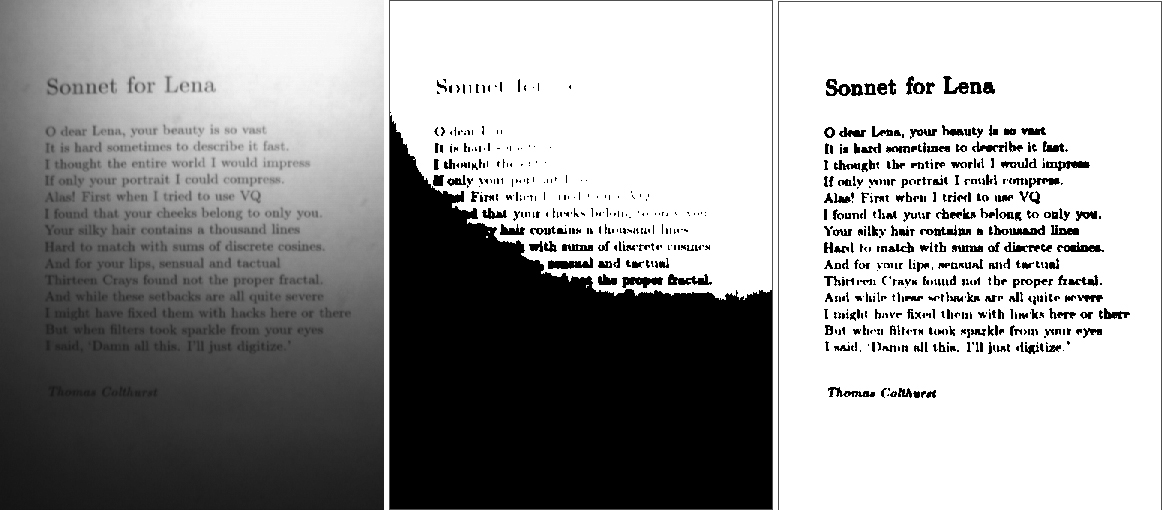
\includegraphics[width=\linewidth]{seuillage.jpg}
\caption{OfBook}
\label{fig:seuillage}
\end{figure}

On comprend ici la bascule entre deux époques de l’OCR. Les anciens systèmes fonctionnaient comme une chaîne d’opérations séparées : on nettoyait l’image, on la binarisait, on comparait chaque forme à une base de motifs connus, puis on s’aidait de dictionnaires pour corriger les erreurs. C’était une sorte de mécanique en plusieurs rouages, où chaque étape pouvait accumuler des approximations. L’OCR, par exemple aux débuts de \emph{Tesseract}, supposait un document déjà segmenté, ce qui impliquait d’appliquer les traitements sur des entrées standardisées \footcite[][]{smith}. Les systèmes contemporains, eux, reposent sur des modèles neuronaux capables d’apprendre l’ensemble du processus de bout en bout : ils prennent une image brute et produisent directement du texte, en intégrant en interne ce qui relevait autrefois de plusieurs étapes distinctes. Cette évolution repose notamment sur les \textbf{LSTM} (\emph{Long Short-Term Memory}), des réseaux dits « récurrents » capables de lire une ligne comme une suite d’images et d’en mémoriser le contexte pour prédire la séquence de caractères. Là où un moteur classique devait isoler chaque glyphe pour le comparer à un modèle, un LSTM fonctionne un peu comme un lecteur humain : il garde en mémoire ce qui précède pour interpréter les lettres suivantes, même quand elles sont collées ou abîmées. Ces architectures ne sont évidemment pas infaillibles, mais elles illustrent de manière exemplaire ce que Simondon appelait la \emph{concrétisation technique}\footcite[][]{meot} : les différentes fonctions du système — nettoyage, segmentation, reconnaissance, correction — deviennent moins séparables et tendent à se fondre dans un dispositif intégré, plus cohérent mais aussi plus opaque. D'un côté, alors, avec le vocabulaire de Gilbert Simondon, on peut dire qu'il y a les dispositifs \enquote{abstraits} des méthodes d'OCR; de l'autre, plus modernes, les dispositifs \enquote{concrets}\footcite[][]{bontems} ou en voie de concrétisation.

Le schème opératoire \enquote{abstrait} -- en \enquote{rouages} -- de la reconnaissance optique des caractères, est décrite dans la littérature des années 1990–2000 comme une architecture en pipeline, où chaque étape de la reconnaissance correspondait à un module distinct : prétraitement, binarisation, segmentation des caractères, classification, puis correction linguistique \footcite[][]{lecolinet}. Dans le cas de \emph{Tesseract} tel que présenté par Ray Smith, le moteur se contentait de prendre en entrée une image déjà binarisée et supposée contenir une seule colonne de texte \footcite[][]{smith}. La reconnaissance procédait alors par extraction des composants connectés, regroupés en glyphes, ensuite soumis à un classifieur géométrique, avant qu’une passe linguistique rudimentaire ne privilégie certaines hypothèses sur la base de dictionnaires ou de listes de fréquences \footcite[][]{smith2013}. Chaque maillon du pipeline pouvait introduire des erreurs, et une approximation en amont — par exemple une mauvaise binarisation ou une segmentation ratée — se répercutait mécaniquement sur l’ensemble de la chaîne. C’est cette architecture séquentielle, héritée des contraintes matérielles et logicielles de l’époque, que les approches contemporaines cherchent à dépasser en privilégiant des modèles neuronaux capables d’apprendre conjointement plusieurs étapes de traitement. Le tournant marqué en 2018 par l’adoption des réseaux LSTM, qui permettent de traiter une ligne d’image comme une séquence continue de signes, a ouvert la voie à une reconnaissance « end-to-end », de l’image brute jusqu’au texte \footcite[][]{smith}. Mais il serait trompeur de croire que cette évolution a entièrement effacé la logique du \emph{pipeline}. Dans la pratique, même les systèmes modernes conservent une structuration en étapes : prétraitement et normalisation des images, segmentation des zones et des lignes, reconnaissance séquentielle avec LSTM ou Transformers, puis décodage et structuration des données -- par exemple avec un export en ALTO/XML -- intégration d’un modèle de langue. Les différences résident moins dans l’existence d’un pipeline que dans son degré d’intégration : là où chaque étape était autrefois codée manuellement, elle est désormais en grande partie apprise ou ajustée automatiquement par le modèle \footcite[][]{pipeline-kraken}. Autrement dit, la chaîne ne disparaît pas, mais elle devient plus compacte, moins visible et plus adaptable, ce qui explique à la fois les gains de performance et la difficulté accrue à contrôler ou interpréter chaque rouage.

\begin{figure}[htbp]
\centering
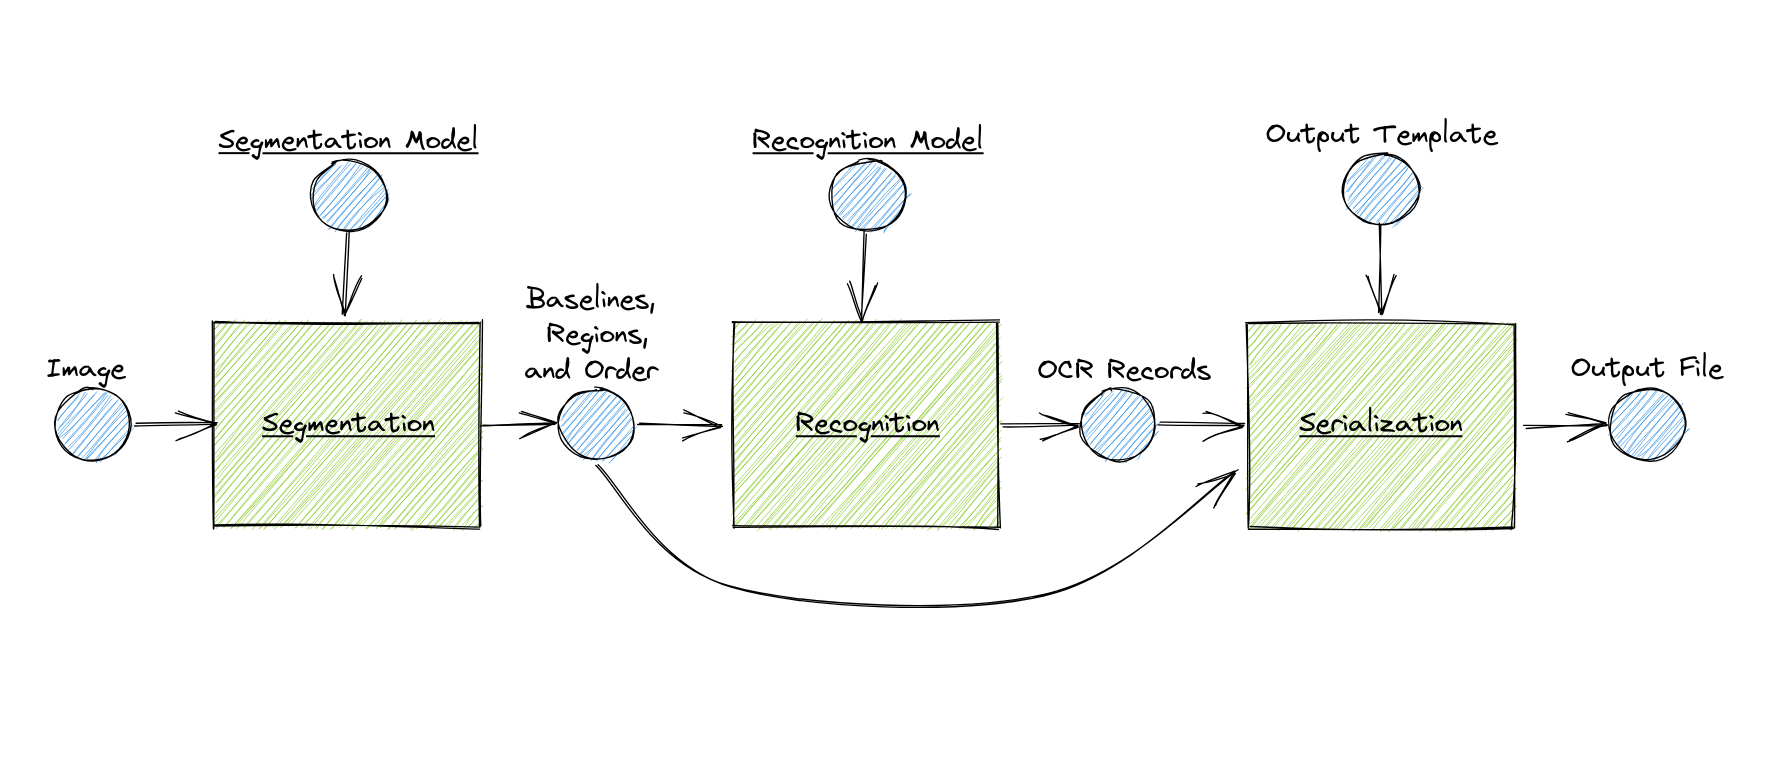
\includegraphics[width=\linewidth]{pipeline-kraken.png}
\caption{}
\label{fig:pipeline-kraken}
\end{figure}

A noter très récemment une nouvelle évolution des pratiques de transcription automatique avec \emph{Mistral OCR}, présentée en 2025 par \emph{Mistral AI}\footcite[][]{mistralocr}. Contrairement aux OCR classiques centrés sur le texte seul, ce modèle est multimodal -- c'est-à-dire qu'ilcomprend simultanément le texte, les images, les tableaux, voire les équations, les assemblages textuels et visuels d’un document, et cela tout en préservant la mise en page et la hiérarchie informationnelle. Il produit une sortie structurée — notamment en Markdown ou JSON —, intercalant texte extrait et formes visuelles (images ou équations), avec préservation de l’ordre des éléments, des titres, des tableaux.

\subsection{Les grandes technologies d'OCR}

Historiquement, les premiers systèmes d’OCR, développés entre les années 1970 et 1990, étaient conçus pour reconnaître des caractères bien standardisés, tirés d’impressions propres ou de typographies contemporaines. Ils se montraient performants tant que les documents étaient homogènes et en bon état, mais trouvaient rapidement leurs limites face à la diversité des fonds patrimoniaux : imprimés anciens, journaux abîmés, écritures non latines ou manuscrits. C’est cette hétérogénéité croissante qui a conduit au développement de solutions spécialisées, plus flexibles et adaptées aux besoins des bibliothèques et des chercheurs.

Parmi ces moteurs, \emph{Tesseract} occupe une place singulière. Développé initialement par Hewlett-Packard dans les années 1980 puis repris par Google, il est devenu l’un des logiciels libres d’OCR les plus diffusés au monde, car utilisé notamment dans de grandes bibliothèques numériques comme \emph{Google Books} et publié en \emph{open-source} en 2005\footcite[][]{smith}. Sa quatrième version, publiée en 2018, a marqué une étape importante en intégrant des réseaux de neurones récurrents -- les LSTM dont on a brièvement parlé précédemment -- ce qui a permis d’améliorer considérablement ses performances sur des typographies variées. Néanmoins, Tesseract reste relativement rigide dès lors qu’il s’agit de traiter des documents abîmés ou des écritures complexes, à l'instar de la typographie vernaculaire ou des écritures manuscrites.

À côté de \emph{Tesseract}, citons le logiciel propriétaire \emph{ABBYY FineReader} au coût élevé et au développement fermé limitant les possibilités de personnalisation. Bien que \emph{Tesseract} soit devenu un standard libre et largement utilisé pour l’OCR typographique, il n’était pas assez flexible pour répondre aux défis spécifiques des corpus patrimoniaux. C’est dans ce cadre que \emph{Kraken} a vu le jour. Conçu dès l’origine pour pouvoir être entraîné sur des corpus particuliers — imprimés anciens, écritures non latines, manuscrits, gazettes, etc. Benjamin Kiessling, dans \emph{Kraken – a Universal Text Recognizer for the Humanities}\footcite[][]{kiessling} décrit comment Kraken élimine les « implicit assumptions on content and layout » propres aux systèmes classiques, tout en permettant l’entraînement d’architectures sur mesure, la reconnaissance de scripts non standards et l’export en formats interopérables tels que PAGE XML ou ALTO XML.

Dans le prolongement de ces initiatives, la plateforme eScriptorium, développée à l’École pratique des hautes études (EPHE/PSL) au sein du projet Huma-Num, combine différents modules de segmentation et de reconnaissance. Elle intègre notamment Pero OCR pour la détection des zones et la segmentation des lignes, et Kraken pour la transcription. eScriptorium offre en outre une interface collaborative qui permet à des équipes de chercheurs, mais aussi à des communautés élargies, d’annoter, d’entraîner et de partager des modèles. Cette dimension participative en fait un outil particulièrement adapté aux humanités numériques, où la correction et l’amélioration collective des résultats constituent un enjeu central.

\subsection{CER, WER : métriques pour évaluer la qualité de l'OCR}

Dans ce contexte, la question de l’évaluation des performances devient cruciale. Si la reconnaissance automatique produit un texte exploitable, il est nécessaire de mesurer la qualité de cette transcription afin d’orienter les corrections, de comparer les moteurs ou de juger de l’efficacité d’un entraînement. Deux indicateurs dominent aujourd’hui dans le champ : le \textbf{CER} (\emph{Character Error Rate}) et le \textbf{WER} (\emph{Word Error Rate}).

Le \textbf{CER} mesure le pourcentage d’erreurs au niveau des caractères. Concrètement, il s’agit de comparer la sortie d’un moteur à une transcription de référence (\emph{ground truth} ou \enquote{vérité terrain}), puis de calculer le nombre minimal d’opérations nécessaires pour transformer l’un en l’autre : substitutions, insertions ou suppressions. Formellement, ce calcul repose sur la distance de Levenshtein, un algorithme de comparaison de chaînes. Le CER s’exprime comme le rapport entre le nombre d’opérations et le nombre total de caractères de la référence. Ainsi, un CER de 5 \% signifie que sur cent caractères transcrits, cinq nécessitent correction.

Le \textbf{WER}, de son côté, transpose le même principe au niveau des mots. Il se révèle souvent plus parlant pour l’utilisateur final, car une seule erreur de caractère peut parfois changer entièrement un mot (« loi » devenu « foi »). Mais il est aussi plus sensible aux fautes d’espacement ou de segmentation, ce qui en limite parfois l’usage sur des corpus anciens où les règles typographiques varient fortement.

Dans la pratique, les projets combinent souvent ces deux indicateurs[David Fleischhacker]. Le CER est préféré pour comparer des modèles entre eux, car il est plus fin et moins dépendant des conventions d’espacement, tandis que le WER donne une estimation plus intuitive de la lisibilité globale d’un texte. Dans des corpus patrimoniaux difficiles (imprimés du XIXᵉ siècle, microfilms, manuscrits), atteindre un CER inférieur à 5 \% est déjà considéré comme un excellent résultat.

Cependant, il faut rester critique au regard de ces métriques. Comme le montre Neudecker[Neudecker], même les mesures dites « standardisées »  -- que sont le CER et le WER -- ne sont pas directement comparables d’un outil d’évaluation à l’autre. Une source d’écart importante réside dans le calcul des alignements, c’est-à-dire la manière dont on fait correspondre, pas à pas, la transcription automatique produite par la machine et la transcription de référence. Selon l’algorithme d’alignement retenu, par exemple un alignement global de type Levenshtein ou un alignement local optimisé, une même séquence de sorties peut être jugée plus ou moins « erronée ». Cela produit des variations sensibles du CER/WER, surtout dans les cas où l’OCR omet des caractères, inverse des espaces ou fusionne des mots. Dans les humanités numériques, un cas typique est celui des corpus de presse ancienne : un OCR peut confondre les colonnes et inverser l’ordre de lecture, ce qui entraîne de longues séquences décalées. Pour l’algorithme d’alignement, ces erreurs se traduisent en cascades de substitutions et d’insertion/suppressions, gonflant artificiellement le CER, alors que pour l’historien intéressé par la recherche lexicale, la reconnaissance des formes de mots resterait partiellement exploitable. Cette discordance montre que CER et WER n’évaluent pas la pertinence de l’OCR du point de vue des usages, mais reflètent seulement une comparaison mécanique. Elle plaide pour le développement de métriques contextualisées capables d’intégrer la segmentation et l’ordre de lecture, dimensions essentielles pour l’exploitation scientifique des corpus patrimoniaux.

\begin{encadre}
\textbf{Calcul du CER et du WER}

Soit une séquence de référence $R$ (le \emph{ground truth}) et une séquence prédite $H$ (hypothèse).
On définit :

\begin{itemize}
\item $S$ : le nombre de substitutions,

\item $D$ : le nombre de suppressions (\emph{deletions}),
\end{itemize}
$I$ : le nombre d’insertions,
\begin{itemize}
\item $N$ : le nombre total d’unités dans la référence ($N = |R|$).

\end{itemize}
La \textbf{distance de Levenshtein} correspond à $S + D + I$, soit le nombre minimal d’opérations nécessaires pour transformer $R$ en $H$.

$$
CER = \frac{S + D + I}{N_\text{caractères}}
\qquad\qquad
WER = \frac{S + D + I}{N_\text{mots}}
$$

\begin{itemize}
\item \textbf{CER} : $N$ correspond au nombre total de caractères de la référence.

\item \textbf{WER} : $N$ correspond au nombre total de mots.
\end{itemize}
Un score proche de \textbf{0 \%} indique une reconnaissance quasi-parfaite ; au-delà de \textbf{20–25 \%}, le texte devient difficilement exploitable sans corrections massives.

\end{encadre}
\subsection{Numérisation du \emph{Journal Officiel} : une politique documentaire partagée entre la BnF et les institutions parlementaires}

En 2009, la BnF a ouvert ses marchés de numérisation aux institutions parlementaires, amorçant un partenariat durable avec le Sénat et l’Assemblée nationale pour la mise en ligne de leurs archives. Ce choix, qui prolongeait le programme de « numérisation concertée » lancé quelques années plus tôt, répondait à un double objectif : préserver des ensembles documentaires fragiles et en garantir la diffusion publique. Le Sénat confia ainsi à la BnF la numérisation de ses \emph{Impressions parlementaires} — débats, rapports, annexes — couvrant la Troisième République : les volumes de 1876 à 1905 et de 1910 à 1940 furent traités en priorité, tandis que la tranche 1906-1909 était encore en cours en 2022 . L’Assemblée nationale engagea un processus similaire pour ses débats et comptes rendus, accessibles à la fois sur Gallica et sur son propre site institutionnel. Ces campagnes illustrent la manière dont les chambres parlementaires ne sont pas de simples « producteurs » de sources, mais de véritables acteurs documentaires : en orientant la sélection, en organisant l’accès et en choisissant les canaux de diffusion (Gallica, Retronews, portails institutionnels), elles contribuent à instituer de nouvelles modalités de visibilité du droit et du débat démocratique.

Le \textbf{Sénat} a entrepris la numérisation de ses \emph{Impressions parlementaires} (débats, rapports, annexes) couvrant la Troisième République. Ces volumes, progressivement intégrés dans Gallica, prolongent la série du \emph{Journal Officiel} et permettent de reconstituer l’activité législative dans toute sa diversité. L’\textbf{Assemblée nationale}, de son côté, a engagé une démarche parallèle avec la mise en ligne de ses débats, à la fois via Gallica et via son propre site institutionnel. Cette articulation produit un maillage documentaire à plusieurs niveaux : d’un côté, Gallica centralise et homogénéise l’accès, dans une perspective patrimoniale ; de l’autre, les sites parlementaires valorisent leurs archives selon leurs propres logiques éditoriales et politiques.

Cette répartition des rôles illustre un modèle hybride de gouvernance documentaire. La BnF définit le cadre et assure l’infrastructure technique ; les assemblées parlementaires apportent leurs fonds et orientent les priorités de mise en ligne. Mais cette complémentarité n’est pas sans tension : les corpus disponibles demeurent lacunaires, et les chercheurs doivent souvent jongler entre Gallica, Retronews et les portails institutionnels pour accéder à une série complète. Comme le notait déjà un guide pratique destiné aux usagers, la consultation du J.O. en ligne exige de composer avec des accès fragmentés et une indexation parfois insuffisante.

En définitive, la numérisation du \emph{Journal Officiel} illustre la logique de coopération encadrée qui structure la politique documentaire française : un équilibre entre centralisation patrimoniale par la BnF et initiatives propres des institutions productrices, ici les chambres parlementaires. Cette articulation garantit la diffusion publique d’un corpus emblématique, tout en révélant les contraintes techniques et les arbitrages qui accompagnent toute politique de numérisation à grande échelle. 

\chapter{Données brutes, données structurées}

On l'a vu : la première étape du processus de datafication de sources numérisées et accessibles via les institutions patrimoniales est celle de l’acquisition photographique : un document est scanné ou photographié. On obtient alors une image, fidèle à la source mais muette du point de vue informatique : elle est lisible par l’œil, mais inerte pour un moteur de recherche. La seconde étape, quant à elle, est celle du passage au texte : grâce à la reconnaissance optique de caractères (OCR), l’image est convertie en une suite de signes alphabétiques. On peut alors effectuer des recherches plein texte, mais ce matériau reste linéaire et peu organisé.

La troisième étape, décisive pour l’analyse, est celle de la structuration. Disposer d’un texte est un point de départ, un pré-requis; mais il s'agit désormais d’identifier dans ce texte des entités, des relations, des attributs — par exemple un nom de sénateur, le sujet de son intervention, le numéro de page correspondant. Ces éléments sont organisés selon un modèle explicite qui rend possible leur comparaison, leur mise en relation et leur analyse. En somme, la structuration est l’opération qui transforme un corpus lisible en données exploitables pour l'analyse. Produire de telles données n’est cependant pas qu’un exercice technique : c’est un travail en trois dimensions — de modélisation (quelle forme donner aux données ?), d’évaluation (comment en juger la qualité ?) et de production (quelles méthodes employer pour transformer un texte en structures fiables ?).

Ce chapitre se concentre sur deux de ces dimensions : comment modéliser des données structurées, et comment les générer à partir de textes. La question de l’évaluation, centrale dans mon stage, quoique abordée ici, fera l’objet d’une partie à part entière.

\section{Modéliser des données structurées}

La première étape consiste à définir la forme que prendront les données une fois extraites. En effet, la notion de « donnée structurée » recouvre plusieurs types de représentations, plus ou moins adaptées selon les usages et les besoins.

Les \emph{ensembles d’enregistrements} (record sets) correspondent au modèle le plus courant : des collections non ordonnées de tuples, analogues à des tables de base de données. Chaque enregistrement associe une série d’attributs décrivant un objet (nom, fonction, date, etc.). C’est ce format qui est généralement mobilisé dans les tâches d’extraction d’information, telles que la reconnaissance d’entités nommées ou l’extraction de relations. Dans les sciences sociales, on le retrouve par exemple dans les recensements de population, où chaque individu est décrit par un ensemble d’attributs (âge, profession, état matrimonial, lieu de résidence), sans que l’ordre des individus ait d’importance. De même, en histoire politique, la constitution d’un corpus de députés ou sénateurs avec leurs mandats, affiliations et interventions peut être représentée sous forme d’un tel ensemble : une « table » de données où chaque ligne correspond à un parlementaire et chaque colonne à une caractéristique descriptive.

Une variante importante est constituée par les \emph{séquences d’enregistrements} (record sequences), où l’ordre des tuples est significatif. Cette organisation ordonnée peut refléter un critère naturel (par exemple l’ordre temporel) ou une convention éditoriale (comme dans un annuaire ou une table nominative). Dans ces cas, la séquence elle-même porte du sens et facilite certaines analyses (suivi de chronologie, validation croisée, etc.). Ainsi, dans les sciences sociales, l’étude des trajectoires professionnelles ou migratoires repose précisément sur ces séquences : l’enchaînement des postes occupés dans une carrière ou des lieux de résidence successifs permet de dégager des régularités collectives, de mettre en évidence des bifurcations ou de comparer des parcours types. De même, en histoire parlementaire, les \emph{Tables Nominatives} du \emph{Journal Officiel} ordonnent les interventions des sénateurs selon l’année et la pagination, offrant une séquence exploitable pour analyser l’évolution des prises de parole dans le temps ou la récurrence de certains thèmes.

D’autres structures plus complexes existent, comme les \textbf{arbres}, qui permettent de représenter des hiérarchies ou des relations imbriquées -- par exemple en analyse syntaxique --, et les \textbf{graphes}, qui offrent une grande flexibilité pour représenter des connaissances consolidées, notamment dans les ontologies ou graphes de connaissances. Ces structures sont néanmoins très intéressantes, car elles bénéficient de solides sophistications mathématiques de la théorie des graphes, de l'algèbre linéaire voire de la topologie appliqué aux données. On peut ainsi détecter des communautés (clustering), mesurer la centralité ou l’influence de certains nœuds dans un réseau, ou encore identifier des chemins de diffusion ou de dépendance entre entités. En sciences humaines, ces méthodes permettent par exemple de reconstituer des réseaux de sociabilité, d’analyser la circulation d’idées ou de suivre l’évolution de liens institutionnels. Néanmoins, l’évaluation de ces structures, en particulier les graphes, dépasse généralement le champ de l’extraction d’information proprement dite.

Dans le cas qui nous occupe, à savoir l’extraction d’informations à partir des documents parlementaires, les \emph{ensembles et séquences d’enregistrements} sont les plus pertinents. Ils correspondent directement à la structure des \emph{Tables nominatives}, où l’on recense des individus (sénateurs), des événements (leurs interventions) et des attributs associés (objets des débats, références de page). C’est donc sur ce type de représentation que nous concentrons notre attention dans la dernière partie du mémoire. Cependant, la modélisation n'est en pratique pas qu'un exercice intellectuel. L'expérimentation nous renseigne et nous permet d'amender la façon de voir les données, de les mettre en relation. Tout dépend de ce à quoi on tient savoir : si la relation entre les sénateurs importent plus que leur trajectoire intellectuelle, alors un graphe sera plus pertinent qu'une séquence d'enregistrements. Encore une fois, la dimension technique de la modélisation repose sur des enjeux valuatifs de la recherche.

\section{Produire des données structurées à partir de texte}

Enfin, la question centrale demeure : comment générer des données structurées à partir de texte brut ? Trois grandes familles d’approches dominent : les approches par \emph{pattern matching}, les \emph{approches extractives} et les \emph{approches génératives} \footcite[][]{graham}.

Les approches par \emph{pattern matching} consistent à rechercher dans un texte brut des séquences de caractères ou de mots qui correspondent à des motifs préalablement définis. Elles reposent sur l’idée que certaines informations suivent des régularités formelles ou typographiques que l’on peut capturer par des règles explicites. Les \emph{expressions régulières} -- ou \emph{Regex} -- en constituent l’exemple le plus connu : elles permettent de détecter des dates, des numéros, ou encore des patronymes en fonction de leur forme. 

Les approches extractives reposent sur l’identification directe, dans le texte, des fragments qui correspondent aux champs d’une structure cible. Elles peuvent être mises en œuvre via des règles (expressions régulières, patrons linguistiques) ou via des modèles supervisés d’étiquetage de séquence, comme les CRF [5] ou les modèles encodeurs-transformers (BERT, RoBERTa) [4]. Ces approches présentent l’avantage de limiter le risque d’hallucinations : elles ne « fabriquent » pas d’information absente du texte, puisqu’elles ne font que sélectionner et classer ce qui existe déjà. En revanche, elles nécessitent un entraînement spécifique à la tâche, ce qui implique un corpus annoté, des ressources computationnelles et du temps.

Les approches génératives, en revanche, considèrent l’extraction comme une opération de traduction : le texte source est « traduit » dans un format cible (JSON, CSV, XML, etc.). Les modèles autoregressifs, et en particulier les LLMs, ont ravivé l’intérêt pour cette voie grâce à leur capacité à généraliser en \emph{zero-shot} ou \emph{few-shot} [1, 20, 21]. Des techniques récentes permettent même de contraindre la génération à respecter des formats prédéfinis, par exemple en filtrant dynamiquement les tokens pour ne retenir que ceux compatibles avec une grammaire donnée [23]. Cette flexibilité rend possible la production de structures complexes et imbriquées, tout en captant des informations implicites. Leur inconvénient majeur reste toutefois le risque d’hallucinations, c’est-à-dire de données inventées ou inférées à tort, souvent difficiles à détecter automatiquement.

Dans notre étude, nous avons choisi d’explorer l’efficacité des approches génératives pour traiter les structures répétitives des \emph{Tables nominatives}. Nous mettons à profit les capacités \emph{zero-shot} des LLMs pour évaluer dans quelle mesure ils peuvent produire des données structurées fiables et interopérables à partir de corpus parlementaires. Cependant, il convient de motiver ce choix en abordant les différentes catégories de générations de données que nous venons de donner.

\subsection{Approche à motifs explicites : les ReGex}

L’une des premières méthodes mobilisées pour extraire de l’information à partir de textes repose sur l’usage des expressions régulières (Regular Expressions, ou RegEx). Développées dès les années 1950 dans le champ de la théorie des automates, elles se sont imposées comme un outil incontournable pour le traitement automatique de texte. Leur principe est simple : définir un motif formel (pattern) qui décrit la forme que doit prendre une séquence de caractères afin qu’elle soit reconnue par le système. Par exemple, un motif tel que \d{4} permet de détecter toutes les occurrences de suites de quatre chiffres, ce qui peut correspondre à des dates dans un texte.

Cette approche présente des avantages certains. Les RegEx sont rapides à exécuter et extrêmement précises dès lors que l’on connaît à l’avance la forme des données recherchées. Elles sont également peu coûteuses en ressources computationnelles et ne nécessitent aucun entraînement supervisé : il suffit de concevoir le motif pour capturer l’information. Dans le cas de documents semi-structurés ou normés (par exemple la détection de numéros de lois, de dates ou de références bibliographiques), les expressions régulières restent un outil efficace. Elles peuvent aussi servir de composant de prétraitement dans des pipelines plus complexes, en nettoyant ou en normalisant certaines informations avant de les confier à des modèles plus avancés.

Toutefois, leur rigidité limite fortement leur portée. La conception d’une RegEx efficace suppose que l’on ait une connaissance préalable de la forme exacte de ce que l’on cherche — or, dans le cas de sources historiques, cette condition est rarement remplie. Les variations typographiques, les abréviations, les fautes de frappe ou encore les artefacts liés à l’OCR (caractères mal reconnus, coupures de lignes, ligatures) rendent les motifs fragiles. Une expression trop stricte manquera des cas pertinents ; une expression trop souple capturera du bruit et produira des faux positifs. Les approches de recherche floue (fuzzy matching) ont été développées pour pallier cette rigidité, mais elles ne permettent que de retrouver ce que l’on connaît déjà à l’avance, et ne s’adaptent pas à des contextes entièrement nouveaux. En d’autres termes, l’approche reste fondamentalement fermée. Elle suppose déjà une connaissance assez fine non pas seulement du \enquote{contenu historique} des sources; mais des suites d'opérations techniques de trandusction informationnelle qui commencent à la transcription de l'acte parlementaire au texte OCRisé, en passant par les processus la composition linotypique des imprimeries du \emph{Journal Officiel} et des stratégies d'acquisition numérique.

L’utilisation des RegEx peut être enrichie par des patrons linguistiques plus élaborés (par exemple des grammaires ou des dépendances syntaxiques), par des listes de référence (ou gazetteers, contenant des noms propres, des toponymes, etc.), ou encore par des règles de post-traitement visant à corriger ou normaliser les sorties. Ces ajouts offrent davantage de robustesse et améliorent la précision, mais ils n’échappent pas au principal écueil : la nécessité de concevoir manuellement l’ensemble des règles, ce qui devient rapidement coûteux et peu scalable à grande échelle. L’avantage de ces approches reste toutefois leur explicabilité : contrairement aux modèles neuronaux, les règles définies sont transparentes et permettent de prédire le comportement du système.

Dans le cadre du \emph{Journal Officiel} et des \emph{Tables nominatives}, l’approche par RegEx peut constituer un point de départ utile pour détecter des éléments aux formats relativement standardisés — comme les numéros de page, les années, ou certaines abréviations récurrentes. Cependant, elle montre rapidement ses limites pour capturer la sémantique implicite : qui parle, sur quel sujet, dans quel contexte. C’est précisément ce passage à une structuration plus riche, allant au-delà de la simple détection de motifs de surface, qui justifie le recours à des approches plus sophistiquées. 

\subsection{Approches extractives : BERT}

Face aux limites des expressions régulières, la recherche est passée à une nouvelle étape : confier à des modèles statistiques puis neuronaux la tâche de repérer directement, dans un texte, les éléments d’intérêt. Le principe est simple à imaginer : c’est comme si l’on entraînait un étudiant à surligner systématiquement les noms de personnes, les dates ou les thèmes dans un document. Chaque mot ou groupe de mots reçoit ainsi une étiquette (« nom de sénateur », « fonction », « numéro de page », etc.), ce qui permet de transformer le texte en une série d’enregistrements exploitables.

Au départ, ces systèmes utilisaient des méthodes statistiques assez rigides : on décrivait chaque mot par ses caractéristiques visibles (comme sa terminaison, sa majuscule initiale, son voisinage immédiat) et le modèle apprenait à reconnaître des motifs. Cela marchait, mais seulement si les données ressemblaient beaucoup à celles utilisées pour l’entraînement.

Avec l’apprentissage profond, on est passé à un niveau supérieur. Les réseaux de neurones « séquentiels » (par exemple les LSTM) sont capables de tenir compte de la phrase entière, et donc de mieux comprendre le contexte d’un mot. Ainsi, le système ne se contente pas de voir que « budget » est un substantif, il comprend qu’il apparaît dans un débat sur les finances publiques.

L’arrivée des \textbf{Transformers}, et en particulier de \textbf{BERT}, a encore changé la donne. Pour vulgariser : BERT lit un texte en tenant compte simultanément de tout son contexte, en regardant à gauche et à droite de chaque mot, comme si le système surlignait en comprenant la phrase entière plutôt que mot par mot. Ce modèle a été entraîné sur des millions de phrases, ce qui lui donne une « intuition linguistique » qu’il peut réutiliser sur de nouvelles tâches, même dans des domaines spécialisés comme les débats parlementaires.

Les avantages sont clairs : ces modèles reconnaissent mieux les entités malgré les variations de style ou les petites erreurs d’OCR, et ils nécessitent beaucoup moins de travail manuel pour concevoir des règles. Cependant, il y a un revers : ils ne fonctionnent bien que si l’on dispose d’un jeu d’exemples annotés pour les entraîner sur la tâche précise (par exemple, un lot de pages du \emph{Journal Officiel} où les sénateurs et les objets d’intervention sont déjà identifiés). Or, produire ces annotations coûte du temps et de l’expertise. De plus, l’entraînement suppose une certaine puissance de calcul (GPU, logiciels spécialisés), pas toujours disponible dans des projets en sciences humaines.

En résumé : les approches extractives modernes comme BERT sont de véritables surligneurs automatiques très performants, mais ils demandent une phase préparatoire coûteuse (annotations + infrastructure). C’est ce qui explique que les chercheurs en histoire ou en sciences sociales se tournent de plus en plus vers les modèles génératifs (LLMs), qui contournent en partie ce verrou.

\subsection{Approches génératives : les LLMs}

L’émergence des \textbf{grands modèles de langage (LLMs)} – tels que GPT, Claude, LLaMA ou Mistral – a transformé le champ de l’extraction d’information. Contrairement aux approches dites extractives, qui consistent à surligner et classer des portions du texte existant, les LLMs reposent sur un principe génératif : ils produisent directement une sortie textuelle, guidée par des instructions. L’extraction d’information n’est donc plus envisagée comme une classification locale, mot par mot, mais comme une reformulation structurée : le modèle lit le texte, en sélectionne les éléments pertinents et les restitue sous une forme organisée, prête à l’analyse.

Le cœur de cette approche réside dans l’instruction donnée au modèle, ce que l’on appelle désormais un \emph{prompt}. Celui-ci peut préciser le type de sortie attendu, qu’il s’agisse d’un tableau, d’un schéma en JSON ou d’une liste hiérarchisée, et inclure des exemples pour orienter la génération. Ainsi, à partir d’un passage du \emph{Journal Officiel} mentionnant « M. Dupont intervient au sujet du budget des chemins de fer (p. 234) », le modèle ne se contente pas d’indiquer les entités en jeu ; il est capable de reconstruire une représentation explicite de l’information, par exemple : `{\enquote{nom}: \enquote{Dupont}, \enquote{sujet}: \enquote{budget des chemins de fer}, \enquote{page}: 234}`. Cette capacité à produire une structure à la volée marque un changement de paradigme. L’utilisateur ne construit plus un modèle spécialisé via un entraînement complexe, mais formule une consigne linguistique à laquelle le modèle s’adapte immédiatement.

Cette approche présente plusieurs atouts. Elle se distingue d’abord par sa flexibilité : un même modèle peut accomplir une grande variété de tâches, qu’il s’agisse d’extraire des entités, de résumer des documents ou de convertir un texte en tableau, sans nécessiter de jeu de données annoté ni d’entraînement spécifique. Elle se caractérise également par sa rapidité de mise en œuvre : quelques \emph{prompts} bien conçus suffisent à obtenir des résultats exploitables, ce qui réduit considérablement les coûts et les délais d’un projet. À cela s’ajoute une robustesse linguistique liée au pré-entraînement massif de ces modèles sur d’immenses corpus : ils reconnaissent des formulations inhabituelles, des variations lexicales ou syntaxiques, et produisent malgré tout une sortie cohérente. Enfin, leur capacité à générer directement dans des formats structurés tels que le JSON, le CSV ou l’XML rend leurs productions immédiatement intégrables dans des bases de données ou des environnements analytiques.

Mais ces avantages ne doivent pas masquer certaines limites. Les sorties générées ne sont pas toujours stables : un même prompt appliqué à des passages similaires peut donner lieu à des structures divergentes, ce qui complique l’automatisation complète du processus. Les modèles sont en outre sujets aux « hallucinations », c’est-à-dire qu’ils peuvent inventer des données absentes du texte original, une dérive particulièrement problématique du point de vue scientifique. La qualité des résultats dépend aussi de la formulation du prompt, qui devient un paramètre méthodologique central et parfois délicat à maîtriser. Enfin, si l’usage ponctuel d’un LLM est peu coûteux, le traitement de corpus volumineux peut rapidement représenter un investissement financier ou technique non négligeable, selon que l’on mobilise des API commerciales ou des modèles libres installés localement.

Dans le domaine des sciences humaines et sociales, ces modèles ouvrent néanmoins des perspectives inédites. Ils permettent d’extraire automatiquement des informations structurées à partir de corpus historiques, en évitant l’étape fastidieuse et coûteuse de l’annotation manuelle. Des expérimentations récentes ont déjà montré leur potentiel pour la transcription, l’annotation ou l’extraction d’entités dans des fonds patrimoniaux. Pour le \emph{Journal Officiel} et ses \emph{Tables nominatives}, ils offrent la possibilité de transformer directement des listes semi-structurées en tableaux exploitables, en capturant les noms des sénateurs, les objets d’intervention et les références paginées. Une tâche autrefois fastidieuse, nécessitant un dépouillement patient et souvent incomplet, devient ainsi automatisable à grande échelle.

En définitive, les approches génératives déplacent le centre de gravité de l’extraction d’information. Là où l’on cherchait auparavant à construire des modèles spécialisés et rigides, il s’agit désormais d’orchestrer une génération encadrée par des consignes précises. Cette plasticité ouvre un champ nouveau pour la capture sémantique des corpus textuels, mais elle suppose d’accompagner leur usage de garde-fous méthodologiques, afin de garantir la fiabilité et la traçabilité des données produites.

\section{La sortie structurée via LLM pour le \emph{Journal Officiel}}

Il est intéressant de revenir sur l'approche générative car c'est celle-ci qui a été retenue. En effet : l’application des approches génératives par grands modèles de langage, dans le cas du \emph{Journal Officiel}, et plus spécifiquement des \emph{Tables nominatives} du Sénat, a l'avantage d'être simple et rapide à mettre en place. Ces tables, qui fonctionnent comme des index annuels de l’activité parlementaire, présentent une organisation qui semble régulière : elles listent les noms des sénateurs, précisent le sujet de leurs interventions et renvoient aux pages correspondantes. Cette apparente homogénéité masque cependant une série de difficultés. Cette partie ne présentera pas les détails techniques, mais quelques enjeux techniques et avantages à considérer, lesquelles seront développés dans la partie suivante. La mise en page, par exemple, peut varier d’une année à l’autre; les noms sont parfois abrégés ou tronqués; et les textes portent les stigmates d’un OCR imparfait, introduisant du bruit ou des confusions typographiques. À cela s’ajoute la diversité des formulations, qui rend incertaine toute tentative de repérage par motifs fixes. Capturer la sémantique de ces tables suppose donc de dépasser la simple reconnaissance de structures formelles et d’accéder à une représentation organisée et exploitable de l’information.

\subsection{Simplicité}

Les LLMs offrent un compromis assez intéressant. Contrairement aux approches extractives classiques, qui nécessitent la constitution d’un corpus annoté et l’entraînement d’un modèle spécialisé, les LLMs peuvent être mobilisés rapidement avec un simple appel d'API. Il suffit de leur fournir quelques exemples de sortie attendue au sein d’un prompt pour orienter leur génération. Cette souplesse en fait une solution pragmatique, adaptée à des projets exploratoires en sciences humaines où le temps et les ressources d’annotation peuvent être limités. Une campagne d'annotation peut être longue voire approximative, sans accord inter-annotateur qui permet de désambuiguiser l'étiquettage des données. De plus, le recours à ces API accessibles ou à des modèles libres déployés localement permet de réduire les coûts techniques initiaux, tout en laissant aux chercheurs la possibilité de se concentrer sur les choix méthodologiques plutôt que sur les contraintes d’infrastructure. 

\subsection{Sortie structurée, génération structurée}

C’est ici qu’entre en jeu une distinction essentielle : celle entre \textbf{sortie structurée} et \textbf{génération structurée}. Dans le premier cas, dit de sortie structurée, on exploite la capacité du LLM à imiter des formats qu’il a déjà rencontrés lors de son entraînement. Au lieu de laisser parler le LLM avec la prolixité qu'on lui connaît, on le « guide » par le prompt en lui imposant un format attendu — par exemple un dictionnaire JSON comportant les champs `{\enquote{nom}: \enquote{...}, \enquote{intervention}: \enquote{...}, \enquote{page}: \enquote{...}}`. Le modèle, plutôt que de produire une réponse discursive en langage naturel, ajuste alors son texte pour respecter ce format. C’est une manière pragmatique et peu coûteuse d’obtenir des données directement exploitables. La génération structurée va un pas plus loin : elle ne se contente pas de guider la sortie a posteriori, mais contraint en amont les chemins de génération possibles. Techniquement, il s’agit d’agir sur les probabilités de production des tokens, en forçant le modèle à n’émettre que des suites de symboles compatibles avec une grammaire donnée, comme JSON ou XML. Cette mise « sur rails » de la génération, qu’on peut comparer à un automate fini qui valide chaque token au moment où il est choisi, permet d’éviter les écarts ou les incohérences de format. Dans mon cas, comme on le verra dans la partie suivante, la première approche aura été choisie : une sortie structurée imposée par le prompt, sans recours à une génération contrainte au niveau des probabilités. L’avantage de ces deux méthodes, et particulièrement de la sortie structurée, est de rendre possible une intégration directe dans des pipelines d’analyse. Le texte brut devient immédiatement une table exploitable ou un ensemble d’enregistrements importables dans une base relationnelle. En outre, cette structuration assure la traçabilité : chaque donnée extraite peut être reliée au fragment de texte d’où elle provient, ce qui rend possible une vérification par l’historien.

Il reste néanmoins essentiel de souligner les limites et les précautions que cette approche implique. Les sorties produites par les LLMs ne sont pas toujours stables : un même prompt appliqué à des passages semblables peut générer des structures divergentes, incomplètes ou incohérentes. Les modèles peuvent aussi souffrir d’« hallucinations », inventant des informations absentes du texte original. Enfin, la qualité des résultats dépend fortement de la formulation du prompt, dont de petites variations peuvent entraîner de grandes différences dans les réponses. Pour ces raisons, la mise en place de protocoles de validation est indispensable. Cela peut passer par un contrôle humain sur des échantillons, par l’application de règles automatiques de cohérence (par exemple vérifier qu’un numéro de page est bien un entier valide), ou encore par l’alignement systématique des sorties avec des référentiels externes, tels que les listes officielles des sénateurs d’une année donnée. Ces garde-fous garantissent que les données produites conservent leur fiabilité scientifique et puissent être mobilisées dans le cadre d’une recherche historique rigoureuse. Une fois obtenues, ces données structurées ouvrent un large éventail de possibilités : suivre longitudinalement l’activité des sénateurs, mesurer la fréquence et la thématique de leurs interventions, ou encore croiser ces informations avec d’autres corpus, tels que les débats parlementaires complets ou les archives législatives. Là où le dépouillement manuel demeurait fastidieux et fragmentaire, la structuration par LLM transforme le \emph{Journal Officiel} en un matériau interrogeable, apte à nourrir des analyses sérielles, des visualisations de réseaux d’intervenants ou des comparaisons thématiques.

Cependant, si l’utilisation des LLMs pour la capture sémantique du \emph{Journal Officiel} constitue une approche pragmatique, combinant rapidité de mise en œuvre et faible coût – notamment parce qu’elle évite la lourde étape d’annotation –, elle comporte des risques majeurs. Les modèles peuvent produire des hallucinations, c’est-à-dire des sorties erronées, incomplètes ou inventées, qui fragilisent leur usage scientifique. Dès lors, l’enjeu central n’est plus seulement de produire des données, mais de mesurer le degré de confiance que l’on peut accorder aux résultats. Cette évaluation doit être envisagée à l’échelle de toute la chaîne de traitement : depuis l’image OCRisée jusqu’aux données structurées produites par le modèle.




%%%%%%%%% PARTIE 3
\part{Expérimenter et évaluer pour comprendre : une démarche historienne outillée}

%\section{Introduction}
\label{sec:intro}
The growing use of artificial intelligence by historians \cite{clavert2024histoire} is multiplying the possibilities for producing historical datasets. The advent of large language models (LLMs) is further changing the landscape, especially for processing textual data corpora, with a proliferation of uses and experiments in the humanities and social sciences\footnote{The "DH@LLM: Grands modèles de langage et humanités numériques" conference program, held in Paris in July 2025, is a good illustration of this: \href{https://www.crihn.org/nouvelles/2025/01/16/colloque-dhllm-grands-modeles-de-langage-et-humanites-numeriques-sorbonne-universite/}{https://www.crihn.org/nouvelles/2025/01/16/colloque-dhllm-grands-modeles-de-langage-et-humanites-numeriques-sorbonne-universite/}}. Zero-shot LLMs are capable of performing a wide range of tasks without the need for task-specific examples or fine-tuning \cite{kojima2022large,wei2022emergent,zhao2023survey} and have demonstrated their ability to carry out many time-consuming tasks in historical research, such as transcription \cite{humphries2024unlocking}, information extraction \cite{knutsen2024alimenter}, or annotation \cite{yuan2025leveraging}. 

%In the context of historical data extraction, a key issue is obtaining structured outputs. While structured generation -- which constrains a Large Language Model to directly produce information in a predefined format like JSON -- is a way to achieve this, a structured output can also be obtained through post-processing of free-form text generation. Regardless of the method, structured output enables the preservation of \joseph{the link to?} the original document and facilitates return to the source, while still allowing for subsequent processing — such as, for instance, integration into a database.

The use of large language models (LLMs) opens new perspectives for extracting structured data \cite{liu2024structured} from historical documents. In the context of historical data extraction, a central challenge lies in obtaining structured outputs. One approach is structured generation, which constrains a large language model to directly produce information in a predefined format such as JSON. Alternatively, structure can be imposed through post-processing of free-form text outputs. Regardless of the approach, producing structured data enables traceability back to the original document and facilitates source verification. It also supports downstream uses, such as integration into a database or further computational analysis.

%\joseph{Est-ce que le problème n'est pas de dire : 1. comment on passe du texte brute au CSV (pour simplifier) et 2. comment on évalue ce que ça donne ?}

%\marie{Si ça vous convient à tous les deux, je trouve ça mieux.}
%\joel{Oui, ça me convient !} \marie{Ci-dessous, une proposition, en ayant utilisé ce qu'a dit Joseph. J'ai aussi utilisé ce qu'il a dit par Teams.}

Two fundamental issues still remain: (1) how to move from raw text to an exploitable structured representation, such as a table or CSV file ; and (2) how to assess the quality and reliability of the extracted data. This article addresses both aspects through a concrete case study: the extraction of structured information from the 1931 \textit{Tables nominatives} or \textit{Tables des noms} of the French Senate (index of senatorial activity ordered by name). We explore a lightly constrained generation approach using an LLM and propose a method to represent the target data, guide the extraction process, and evaluate system performance. Beyond this specific case, the study aims to contribute to broader reflections on the feasibility and limitations of generative models for structuring historical data.

The \textit{Tables des noms} of the French Senate was published during the French Third Republic (1870–1940)\footnote{These tables are part of the \textit{Tables annuelles} (yearly activity index), which can be consulted on the digital library of the French national library (\textit{BnF}): \href{https://gallica.bnf.fr/ark:/12148/cb371291967/date.item}{https://gallica.bnf.fr/ark:/12148/cb371291967/date.item}.}.
Within the broader documentary ecosystem of the \textit{Journal Officiel} ---~which seeks to reconstruct parliamentary activity and its legal or regulatory outcomes in France~---, the Senate's \textit{Tables nominatives} offer a concise and systematic record of senators' interventions during public sessions.
These indexes were designed to accompany the transcription of debates\footnote{The complete transcriptions of Senate debates can be consulted via Gallica: \href{https://gallica.bnf.fr/ark:/12148/cb34363182v/date}{https://gallica.bnf.fr/ark:/12148/cb34363182v/date}.} and to facilitate their consultation.
Manually compiled once a year, they recorded each intervention by senators or members of the government who spoke during the sessions, the subject of their speech, and the corresponding page number.
%
While these tables were particularly useful at a time when full-text search in digitized parliamentary debates was not possible, they still hold significant value for historians today.
Systematically extracting data from them would make it possible to track parliamentary activity over the long term, quantify the interventions of specific senators affiliated with particular political movements, or support the cross-validation of named entities extracted from the debates themselves.
%
Our objective is to extract structured data from these \textit{Tables}; for our initial experiments, we focus on a single \textit{Table nominative}, namely that of 1931.
The early 1930s marked the beginning of the decline of French parliamentarism, culminating in the fall of the Third Republic in 1940 \cite{morel2024parlement}. Analyzing the 1931 \textit{Table} allows us to lay the groundwork for a broader study that will extend across the entire decade, with the aim of capturing the parliamentary activity of the Senate and, subsequently, of the Chamber of Deputies.


%\textbf{Problem:} \textit{[bon là, la 1ère phrase, j'ai un peu riffé... Je ne sais pas si c'est vrai]} Yet, the evaluation of these outputs remains dominated by symbolic “exact match” metrics: Exact Match, Precision/Recall/F-score at the node or parent-child pair level. These metrics are blind to semantic proximity: a predicted label that differs by just one level in the hierarchy or by a lexical variant is penalized as heavily as a completely unrelated prediction, which distorts the measurement of actual performance.

%\joseph{Partie trop technique pour l'intro selon moi, à déplacer dans la partie "Evaluation Framework"}

%\marie{Dans ce cas, il faut supprimer la Research question et enchaîner direct ensuite sur Case study}

%\textbf{Hypothesis:} Optimal Transport (OT) provides a mathematical framework to measure the minimal cost of transforming one distribution into another: here, the distribution of labels generated by the LLM versus the ground truth. By assigning a cost proportional to the semantic/hierarchical distance between labels, OT softens the penalty: the closer the prediction, the lower the cost. The originality of this case study lies in the combination of OT + structured output, which is rarely explored for document indexing tasks. 

%\textbf{Research question:} To what extent does Optimal Transport offer a more fine-grained, human-aligned evaluation than classical metrics when assessing the structured output of an LLM on a document indexing task?

%\textbf{Case study:} Senate tables. Brief presentation of the source and its usefulness.


After reviewing existing approaches to structured data extraction and evaluation (Section~\ref{sec:related-work}), we present three main contributions.

\chapter{L'outil Corpusense : une chaîne de traitement pour les sources historiques}

L’outil \emph{Corpusense} du projet Mezanno a pour ambition de proposer aux chercheurs et chercheuses en sciences humaines et sociales un dispositif dédié à l’exploitation de corpus d’archives sérielles. Là où la partie précédente du mémoire a montré la diversité des enjeux liés à la numérisation et à la mise à disposition de ces sources — qualité imparfaite de l’OCR, absence de structuration exploitable dans les textes bruts, masse de données qui rend toute saisie manuelle irréaliste — \emph{Corpusense} vise à apporter une réponse technique réaliste. \enquote{Réaliste}, car il s’appuie pour cela sur des briques logicielles déjà disponibles et rapides à mettre en place, qu’il agence en une chaîne cohérente correspondant au schème opératoire transcriptif défini précédemment, allant de la source numérisée à la donnée structurée.

Le fonctionnement de \emph{Corpusense} repose principalement sur l’usage d’\textbf{API}, c’est-à-dire d’interfaces de programmation qui permettent à des logiciels hétérogènes de communiquer entre eux en suivant un protocole défini. Les API fonctionnent comme des guichets d'information qui délivrent, selon les requêtes, des données demandées, par exemple une série d'images et leurs métadonnées dans le cas de \textbf{IIIF}. Plutôt que de réimplémenter des modules complexes, l’outil tire parti de services spécialisés en les appelant directement via leurs API. Trois d’entre elles structurent le dispositif : IIIF, donc, qui est le standard largement adopté par les institutions patrimoniales, qui permet de charger et manipuler des images numérisées de manière normalisée. La constitution de corpus se fait donc à partir des dépôts d'archives numérisées, en général par des institutions patrimoniales. Il faut compter également une \enquote{APIsation} du moteur \textbf{Pero OCR} par l'EPITA; qui fournit comme on l'a vu une reconnaissance optique des caractères adaptée aux corpus historiques et multilingues. Et, enfin, l’API de \textbf{Mistral}, un modèle de langage, mobilisée pour transformer les textes OCRisés en sorties structurées adaptées aux besoins des chercheurs (voir \ref{fig:corpusense}). Ainsi, il s'agit de reconstituer une chaîne opératoire, composé de différentes briques agencées et constituées en outil.

\begin{figure}[htbp]
\centering
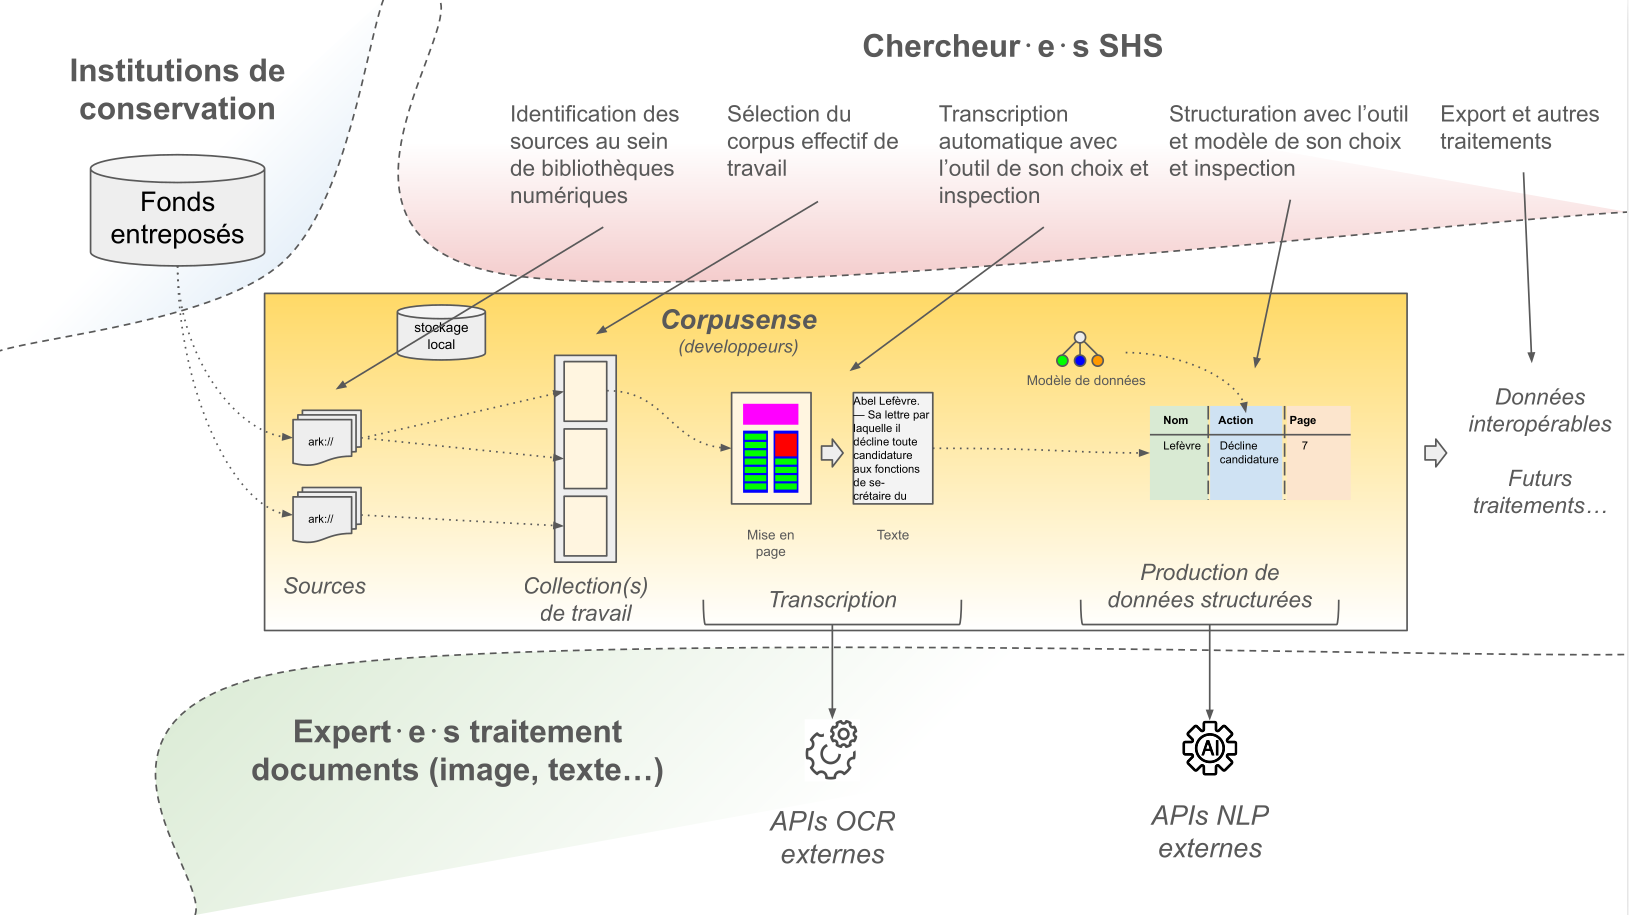
\includegraphics[width=\linewidth]{corpusense.png}
\caption{}
\label{fig:corpusense}
\end{figure}

L'outil motive donc une double orientation. D’une part, il repose sur une chaîne de traitement unifiée, pensée pour transformer des documents d’archives sous forme image en données structurées, interopérables et prêtes à être analysées. D’autre part, il se veut flexible et accessible, de façon à laisser aux chercheurs SHS une autonomie réelle dans la conduite de leurs travaux. Concrètement, une application Web comme \emph{Corpusense} permet de constituer des corpus documentaires à partir de dépôts variés d’archives numérisées et d’y appliquer, sans compétences techniques avancées, des traitements qui aboutissent à des données exploitables.

\section{Une instance de pipeline \enquote{classique}}

L’objectif de Corpusense veut fournir une infrastructure technique robuste pour solidariser les différents rouages (à savoir la constitution des corpus, OCR, extraction) \ref{fig:pipieline_mezz}.

\begin{figure}[htbp]
\centering

\includegraphics[width=\linewidth]{pipieline_mezz.png}
\caption{}
\label{fig:pipieline_mezz}
\end{figure}

La chaîne de traitement se déploie en plusieurs étapes successives. Tout d'abord, la sélection et organisation des sources. Le point de départ réside dans la constitution du corpus. Celui-ci peut provenir de fonds institutionnels (par exemple Gallica, la BnF ou des archives universitaires), ou de collections numérisées indépendantes. Les documents, le plus souvent disponibles sous forme d’images, sont alors recensés et organisés dans un format exploitable. Dans ce contexte, \emph{Corpusense} s’appuie sur le protocole IIIF, largement adopté dans le domaine patrimonial. IIIF permet non seulement d’accéder aux images numérisées de manière normalisée, mais aussi de les manipuler (zoomer, rogner, annoter) et de les intégrer de façon homogène, quelle que soit l’institution d’origine. Ce recours à un standard interopérable assure la portabilité des corpus et facilite leur exploitation au-delà du cadre spécifique de ce projet. 

Ensuite, la transcription par OCR. La deuxième étape consiste à convertir ces images en texte grâce à un moteur de reconnaissance optique de caractères (OCR). Corpusense s’appuie principalement sur le moteur PERO OCR. 

Enfin, la sortie structurée (avec l'API Mistral), laquelle produit un document en JSON, qui peut d'ailleurs être converti aisément en format CSV.

Le choix du format JSON pour représenter les données structurées ne relève pas seulement de la contrainte imposée par l’API Mistral même si cette disponibilité oriente un tel choix. Ce format présente en fait plusieurs avantages décisifs dans le cadre d’un outil comme \emph{Corpusense}. D’un point de vue technique, JSON est un standard commun pour l’échange de données : léger, lisible par l’humain, directement exploitable par la plupart des langages de programmation et facilement convertible en d’autres formats, qu’il s’agisse de tables ou de bases de données relationnelles ou documentaires. Cette plasticité garantit la réutilisation des résultats, quel que soit l’environnement de recherche dans lequel ils sont ensuite mobilisés. L’intérêt du JSON réside dans l'implémentation de la dialectique clé/valeur, laquelle se prête particulièrement bien à des tâches \enquote{indexatoires}, davantage convenante à la logique tabulaire, plus rigide. Là où un tableau, par exemple au format CSV, oblige à « aplatir » l’information, JSON permet de conserver les relations entre entités (par exemple entre un intervenant et les différentes pages où il est cité) et d’accueillir des variations de granularité sans perdre la cohérence du tout. Par exemple, chaque sénateur peut intervenir un certain nombre de fois : en JSON, chaque référence d'intervention est un élément manipulable, distinct des autres; et l'ensemble de ces références est une liste de taille variable. Dans un tableau, on pourrait soit agréger ces différentes références dans une unique colonne séparés avec un séparateur arbitraire \ref{fig:comparaison} -- impliquant alors de parser \emph{a posteriori} ces séries de nombres -- ou bien, mais c'est ici une option assez malheureuse, de constituer autant de colonnes que d'interventions. La séparation des valeurs en JSON fait partie de sa grammaire quand, côté tables, la séparation de valeurs numériques est en fait une chaînes de caractères qu'il faut \enquote{spliter} pour retomber sur une certaine modularité.

\begin{figure}[htbp]
\centering
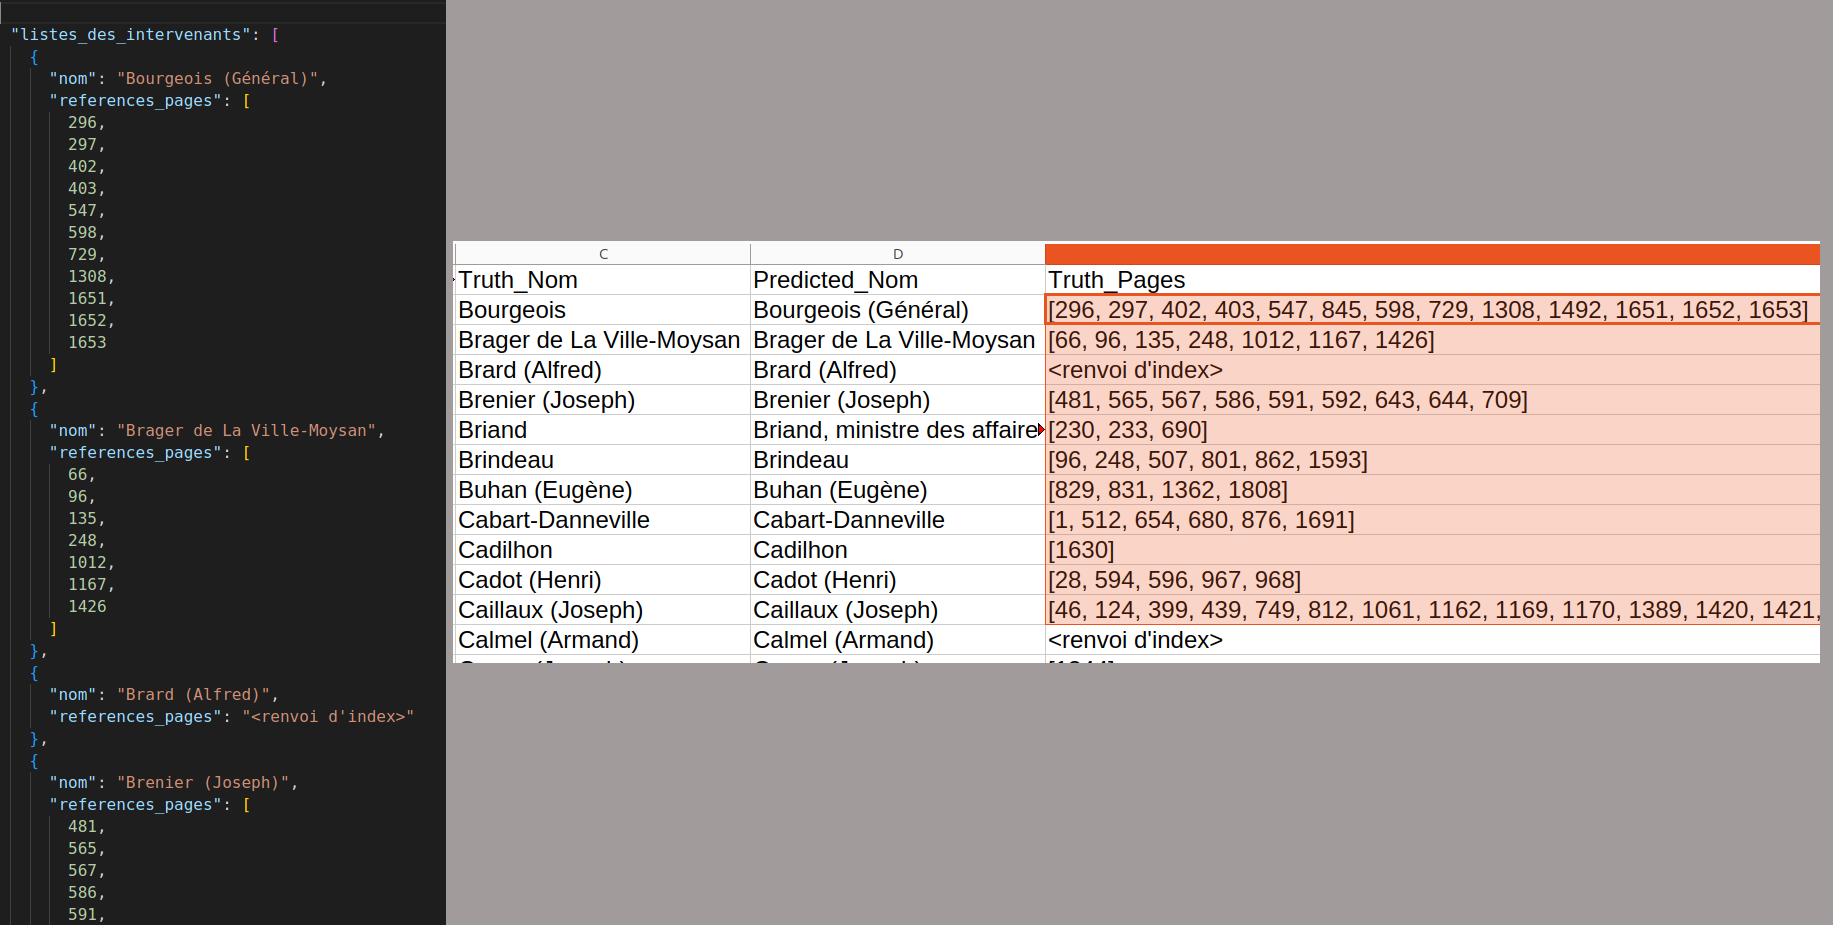
\includegraphics[width=\linewidth]{comparaison.png}
\caption{Comparaison}
\label{fig:comparaison}
\end{figure}

Il est ainsi possible de représenter des cas simples ou complexes au sein d’un même corpus, ce qui correspond mieux à la réalité hétérogène des archives numérisées. A ce stade, on remarque une difficulté pour l'historien qui mobilise des données structurées. Dans une démarche outillée, par exemple avec l'outil \emph{Corpusense}, elle résiderait peut-être moins dans la capacité à programmer qu'à envisager la forme des données, qu'à modéliser un problème ou un ensemble de faits. Cet exercice n’est pas trivial : veut-on décrire des entités et leurs attributs, suivre leur activité dans le temps, ou cartographier leurs relations ? Chacun de ces choix renvoie à des modèles de données distincts, et donc à des manières différentes de faire parler les sources. L'outil ne fait pas disparaître les problématiques de modélisation des données. On retrouve ici la notion de \emph{valuation} au sens deweyien : les moyens de l’enquête — ici, la forme des données et les dispositifs techniques qui les produisent — dépendent des fins poursuivies, mais ces fins elles-mêmes ne sont jamais figées. Elles peuvent être révisées, ajustées ou enrichies au fil des expérimentations, en fonction de ce que les données rendent possible ou non. En ce sens, modéliser les données revient parfois à réactiver, au présent, des gestes interprétatifs analogues à ceux que Collingwood décrivait sous le terme de \emph{reenactment} : l’historien ne fait pas que collecter des informations, il rejoue l’acte de pensée, reconstruit les problèmes tels qu’ils se posaient aux acteurs du passé, mais à travers des médiations techniques. L’historien n’a donc pas affaire à une simple « conversion numérique » de sa pratique, mais bien à une reconfiguration de ses schèmes interprétatifs sous l’effet des opérations techniques. Dans cette perspective, parler de « numérisation du métier d’historien » \footcite[][]{poublanc} ne désigne pas seulement une facilitation instrumentale par les outils numériques : cela renvoie à l’intégration de nouveaux schèmes techniques dans l’enquête elle-même, qui orientent la manière de modéliser les mots et les faits. L’historien ne saurait être l'aliéné des dispositifs techniques — au sens où Simondon entend l’aliénation comme l’usage aveugle d’outils méconnus — mais participe au contraire à leur individuation, en les inscrivant consciemment dans son milieu de recherche et dans ses gestes interprétatifs. 

De plus, cette solidarisation des différentes briques techniques — de cette médiation technique pour constituer des questions et des réponses — ne fait pas disparaître la question de l’évaluation des données produites. Au contraire, elle la rend plus pressante. Car exploiter scientifiquement des données issues d’un assemblage \emph{abstrait} de techniques \emph{concrètes} — pour reprendre le vocabulaire de Gilbert Simondon — suppose de fonder une confiance raisonnée : confiance dans les outils choisis, dans la cohérence de la chaîne opératoire, mais aussi dans la capacité des chercheurs à expliciter les conditions de production des données qui alimentent leur analyse. Dans le cas d’une pipeline comme \emph{Corpusense}, on a affaire à un tel assemblage abstrait : une juxtaposition de fonctions spécialisées (OCR, segmentation, structuration), qui ne forment pas encore un objet intégré mais dont la coopération doit être évaluée comme un tout. Ce qui permet de fonder cette confiance est donc l’\emph{évaluation} de la chaîne de traitement, c’est-à-dire à la fois la performance de chaque module et la cohérence globale de l’ensemble.

\section{Le travail sur Corpusense}

Au moment du stage, \emph{Corpusense} était encore en cours de développement; toutes les fonctionnalités n'étaient pas encore disponibles. Je l’ai donc utilisé principalement pour la constitution du corpus, l’OCRisation et le téléchargement du texte issu de la \emph{Table nominale} de 1931. En revanche, pour la génération de la sortie structurée à l’aide de l’API Mistral, je travaillais directement depuis mon ordinateur, en effectuant les appels manuellement. Cette fonctionnalité est aujourd’hui intégrée dans \emph{Corpusense}, mais elle ne l’était pas encore au moment de mes expérimentations.

Ce décalage n’affecte pas la validité des travaux réalisés : les modules sollicités -- notamment Mistral pour la production JSON -- sont identiques, seul le mode d’appel diffère. Les expérimentations sur la structuration des données ont donc été conduites à partir du texte brut, en dehors de l’application, mais elles prolongent directement le schème opératoire mis en place par \emph{Corpusense}.

\section{Ateliers à l'EHESS et à la BnF}

Avant de passer à l’évaluation proprement dite, arrêtons-nous sur un cas concret qui illustre bien les difficultés rencontrées. Lors d’un atelier mené à l'EHESS par les développeurs de \emph{Corpusense}, une chercheuse — sans formation particulière en informatique — a expérimenté l’outil sur un corpus de la Quatrième République. En une demi-heure, elle a pu obtenir un jeu de données massif, comprenant plus de 1200 entités liées à l’activité parlementaire, plus précisemment sur la production de documents parlementaires. L’exercice montre à quel point la chaîne de traitement peut être efficace et accessible : un travail qui aurait pris des semaines en dépouillement manuel est désormais réalisable en un temps réduit. 

Cependant cette réussite apparente masque plusieurs écueils. La chercheuse, tâche peu facile oblige, a eu du mal à définir précisément son modèle de données : quelles entités retenir ? quelles relations considérer comme pertinentes ? quelle granularité adopter ? Faut-il penser en terme d'acteurs ? De documents produits ? Il a fallu essayer différents modèles pour obtenir un résultat satisfaisant ; redéfinir clairement ce que l'on tenait à savoir sur la période étudiée. On pourrait, en reprenant le mot de Leroy Ladurie, l'historien a tout intérêt à être \emph{designer} -- plutôt d'ailleurs que \enquote{programmeur} -- car l'enjeu est d'être capable de modéliser des données. De plus, même si la structuration a fonctionné, la question centrale reste ouverte : les données ainsi produites sont-elles fiables ? Dans quelle mesure peut-on leur faire confiance pour alimenter une enquête historique, et non seulement une démonstration technique ? A l'issue de cet atelier, qui visait avant tout à expérimenter l'outil qu'à produire de véritables données pour une question de recherche déterminée, le besoin de savoir si les données était fiables était urgent : ainsi, par ce cas exemplaire qui ne fait qu'illustrer une problématique qui a fondé les tenants et aboutissants du stage, la grande question de l'\emph{évaluation} et de la confiance que l'on peut porter aux données.

\chapter{La sortie structurée via LLM appliquée à la Table des Noms du Sénat : une approche empirique}

La pertinence scientifique des analyses repose sur l'évaluation qui ne se réduit pas à un simple contrôle technique. Elle engage une véritable réflexion méthodologique. Dans le cadre du stage, cette réflexion méthodologique s'est adossée à l’expérimentation sur la façon d'évaluer des données, générées par la pipeline. Evaluation et expérimention peut sembler antinomiques. Par évaluation, on entend une dimension scientifique, protocolaire. La notion de \enquote{créativité} que motive au fond celle d'expérimentation et sa dialectique de l'essai-erreur, ne semble pas de mise. Pourtant, la question de la métrique à laquelle s'adosse l'évaluation ne va pas de soi : car il faut évaluer à la fois l'indexation du contenu par le système technique; mais également sa structure de façon conjointe. Il faut également pouvoir apprécier les abscences, les hallucinations; éventuellement, les différentes façons d'OCRiser le texte, tester si un OCR réputé parfait conduit à des résultats finalement très proches de données très imparfaites. De plus, l'évaluation s'adosse à des \emph{vérités terrain} qui, comme on l'a vu pour l'OCR, forment un domaine de référence sur laquelle quantifier les écarts avec la génération du LLM. Ces vérités terrain, qui permettent de fonder une analyse permettant d'émuler l'objectivité, sont pourtant le fruit de décisions qui ne sont pas évidentes : comment nommer ses métadonnées, quelle structure -- ou \emph{schéma} -- conviendrait le mieux à nos données ? La modélisation, comme on vient de le voir également est une véritable affaire de design. Il y a donc un arsenal de paramètres à prendre en compte. Pour arrêter un protocole d'évaluation, il faut dégager des critères de façon empirique -- et donc expérimenter et réduire les paramètres selon ce qu'il semble le plus pertinent. Le mot de Gaston Bachelard selon lequel les instruments seraient de la \enquote{théorie réifiée} est particulièrement approprié à notre cas, car les moyens pour mesurer la qualité des données produites par la pipeline dépend de nos valuations. Cette évaluation prend sens dans un processus itératif où techniques et de valeurs amendées par l'expérimentation et par les objectifs fixés par une question de recherche.

Bien évidemment, cette expérimentation-évaluation s'adosse, non pas à une problématique technique pure, mais à une question de recherche en histoire -- bien qu'elle soit un motif pour guider l'exploration documentaire et computationnelle --, à savoir : cartographier l'activité parlementaire pour l'année 1931, conformément au \emph{reeanctement} collingwoodien suggéré en première partie de ce mémoire sur la qualité du débat parlementaire. Cette motivation historienne, en quatre mois seulement, ne saurait être mené de bout en bout. L'enjeu est donc de maîtriser et évaluer le protocole d'extraction; de tester sa complexité et vérifier qu'il est satisfaisant à ce stade, avant de mener des projets plus ambitieux.

\section{Expérimentations}

\subsection{Prise en main intuitive du problème de la génération de données}

L’expérimentation menée s’est organisée autour de deux volets complémentaires : d’une part, la génération de données à partir des \emph{Tables} parlementaires proprement dite; et, d’autre part, leur évaluation à l’aune d’une vérité terrain soigneusement construite.

Dans un premier temps, le travail a consisté en une phase d’exploration technique visant à s’approprier la tâche d’évaluation des sorties structurées produites par un modèle génératif. L’objectif principal était de vérifier la faisabilité d’une extraction fiable des informations essentielles : les noms des intervenants au Sénat (qu’il s’agisse de sénateurs ou de ministres interpellés) et les dates de leurs interventions.

Ces dates ne figurent pas explicitement dans les \emph{Tables} ; elles doivent être déduites par le biais des références de page, lesquelles constituent des indicateurs temporels indirects. En d’autres termes, la pagination continue du \emph{Journal Officiel} rend possible un fléchage des interventions dans le temps, en reliant chaque entrée des tables à la séance correspondante comme on le verra en temps venu.

Pour produire les données structurées, plusieurs pistes ont été explorées. La plus immédiate a été de recourir à des prompts « naturels » en utilisant directement l'interface Web de Mistral, laissant au modèle une certaine liberté interprétative dans sa réponse. 

\begin{figure}[htbp]
\centering
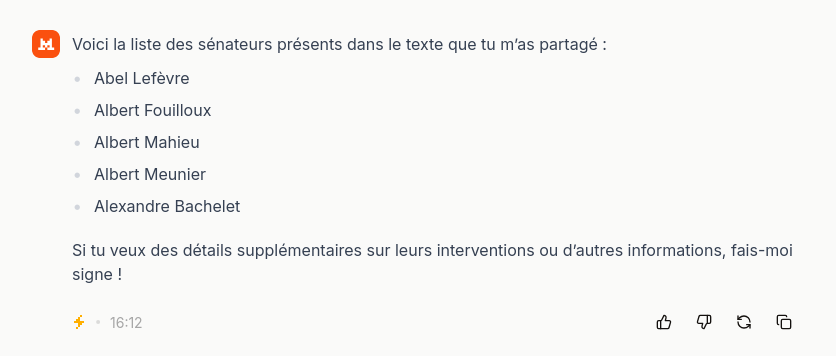
\includegraphics[width=\linewidth]{mistral.png}
\caption{Illustration du résultat d'un prompt avec Mistral (en simulant le modèle disponible en avril 2025) où je soumets un extrait des Tables OCRisées. Comme on le voit, c'est un résultat qui mélange une liste de sénateurs et politesses qui sont ici inconvenantes à une extraction sémantique systématique.}
\label{fig:mistral}
\end{figure}

L'extraction d'une réponse dans l'environnement d'un chat résiste à l'extraction systématique, notamment parce qu'elle est entourée de politesses qui se surajoutent à l'information  qui nous intéresse -- ici la liste des sénateurs \ref{fig:mistral} . Mais également parce que cette réponse est émise dans un environnement -- en ligne -- qu'il est difficile à intégrer dans une pipeline. Les appels à l'API Mistral permettent donc à la fois d'interroger un LLM comme on l'a fait, mais depuis un script qui peut récupérer les données, les sauvegarder en local, d'appliquer divers traitements.

Ce qui nous permet désormais de justifier l’usage de Mistral : l’appel à l’API était gratuit, sans restrictions, et supportait la génération par sortie structurée -- c’est-à-dire la capacité de contraindre le modèle à suivre un schéma formel représentant nos données. Autrement dit, on peut utiliser, sans aucune installation ou dépense, un LLM pouvant être \enquote{contraint} à formuler du JSON -- et rien que du JSON -- par un schéma formels afin de produire des objets comparables. De fait, ce schéma \ref{fig:modelepy} était produit avec la librairie Pydantic qui permet de convertir des classes Python qui représentent le schéma de données, en modèle JSON.

\begin{figure}[htbp]
\centering
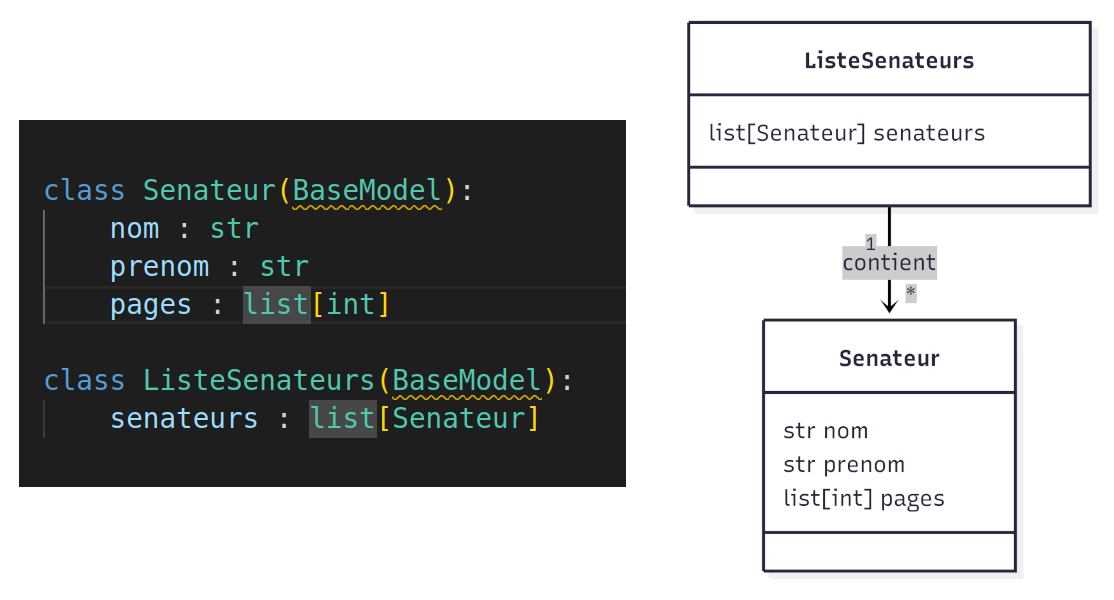
\includegraphics[width=\linewidth]{modelepy.png}
\caption{A gauche, l'implémentation en Pydantic via Python d'un des premiers modèles de données imaginé pour la génération guidée (à droite).}
\label{fig:modelepy}
\end{figure}

Mais un schéma, à lui seul, ne suffit pas : il doit être combiné à un prompt qui guide le modèle. Le tout premier essai reposait sur des instructions très simples :

\begin{quote}
« Extrayez les informations du texte fourni. Je veux la liste des noms et prénoms de toutes les personnes mentionnées (des sénateurs). »  
« Attention au bruit : tout ce qu’il y a dans le texte n’est pas forcément un sénateur. »  
« Voici mon texte : »

\end{quote}
Ces instructions rudimentaires avaient pour objectif principal de vérifier le bon fonctionnement de l’appel à l’API et le retour des données dans le format JSON. En pratique, le pipeline consistait en un script Python qui, à partir du texte OCRisé, soumettait au modèle Mistral un prompt et un schéma, puis récupérait les données produites \footcite[][]{pipeline_mezz}.

Toutefois, dès les premiers tests, des limites sont apparues : les clés choisies dans le modèle, comme \emph{ListeSenateur} ou \emph{Senateur}, étaient trop restrictives. Or, les \emph{Tables nominatives} ne mentionnent pas seulement des sénateurs, mais également des ministres interpellés ou intervenants extérieurs. Un schéma trop strict risquait donc d’induire des omissions. Pour contourner ce problème, il a été décidé d’adopter un vocabulaire plus fonctionnel, centré sur les \emph{intervenants} plutôt que sur une fonction institutionnelle définie de façon explicite. Une fois cette chaîne de traitement permettant de produire des données essayée, il était l'heure de consolider un protocole d'évaluation de cette méthode de génération de métadonnées.

\subsection{Design, prompt et vérité terrain : trouver le bon modèle de données}

Un second volet des expérimentations a porté sur la construction de la vérité terrain, élément indispensable à toute évaluation. En théorie, elle sert de référence absolue pour mesurer les performances du modèle. En pratique, elle résulte d’une série de décisions éditoriales et méthodologiques qui influencent directement les résultats. L’exemple de Louis Barthou, sénateur et ministre de la Guerre en 1931, illustre ce point : fallait-il regrouper toutes ses interventions sous une seule entrée ou distinguer ses apparitions selon ses fonctions \ref{fig:barthou}  ? Le choix de la granularité maximale – séparer chaque occurrence – prévient les confusions d’homonymes, mais complique l’évaluation en raison de la tendance du modèle à fusionner les mentions.

\begin{figure}[htbp]
\centering
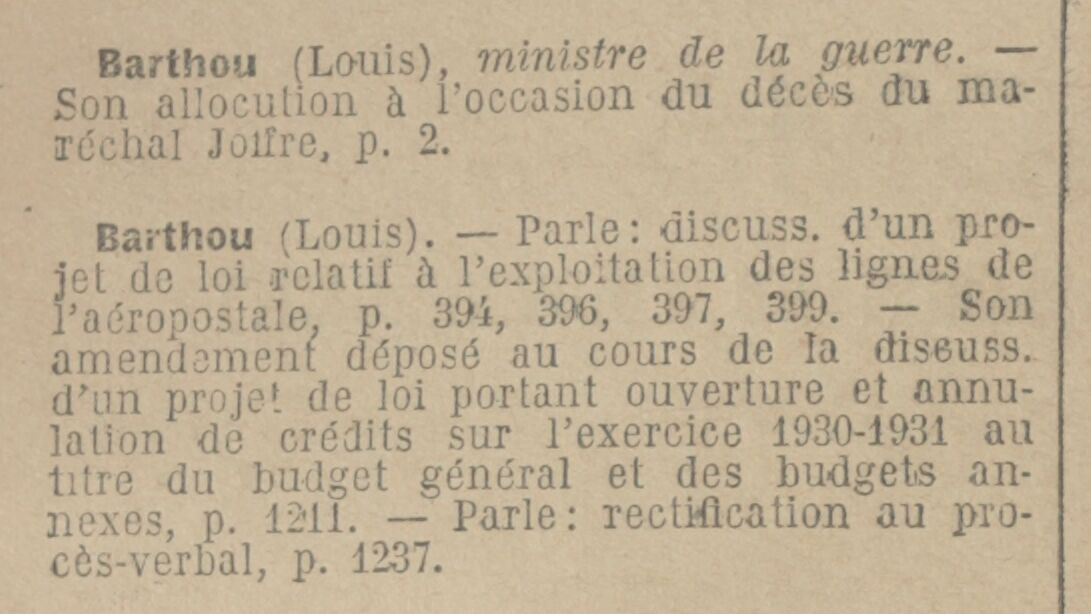
\includegraphics[width=\linewidth]{barthou.jpg}
\caption{}
\label{fig:barthou}
\end{figure}

Sur le plan technique, la vérité terrain est lié au prompt et au schéma de données (\ref{fig:modelpy}). Le schéma de données fait office de \enquote{carte} qui vient guider la production textuelle du LLM. Il indique \enquote{où} mettre les bons mots dans les bonnes boîtes, les bons intitulés avec les bonnes clés. Pour éviter de démultiplier les paramètres à tester, le prompt (voir : ANNEXE 31) et le schéma (ANNEXE 32) ont été stabilisés à l'issu d'un processus itératif pour évaluer la granularité adéquat. Dans le cadre de l'évaluation, seul le nom du sénateur et les pages de références ont été retenues. Pour guider au mieux la génération du JSON par le LLM, on ajoute à notre schéma des descriptions pour qu'il puisse être plus attentif pour qu'il puisse plus facilement mettre les données dans les bonnes boîtes \ref{fig:model}.

\begin{figure}[htbp]
\centering
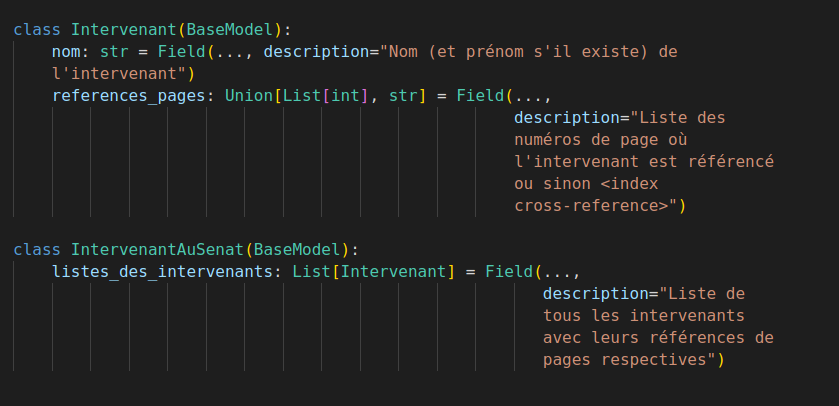
\includegraphics[width=\linewidth]{model.png}
\caption{}
\label{fig:model}
\end{figure}

Le schéma (\ref{fig:model}) joue donc ici le rôle de grammaire opérationnelle : il décrit précisément la structure attendue des sorties (nom, rôle et références paginaires des intervenants), et contraint le modèle à produire un JSON validable. Les premières clés (« Senateur », « ListeSenateur ») ont rapidement montré leurs limites : elles risquaient l'invisibilité d’autres acteurs -- comme les ministres -- et biaisaient l’extraction. La version finale de la vérité terrain (ANNEXE 33) adopte des catégories plus neutres (« Intervenant »), révélant que la modélisation n’est jamais un simple exercice technique mais un choix interprétatif.

Quant aux données produites automatiquement par cette chaîne de traitement stabilisées et appliquées sur l'ensemble des pages des \emph{Tables} du Sénat de 1931 (extraits en annexe : ANNEXE 34) , elles semblent être cohérentes. Mais, à défaut d'évaluation, on ne pas tirer de conclusion décisives.

\subsection{Préparer l'évaluation : comparer, apparier}

L’évaluation des sorties structurées générées par un LLM reposant sur un schéma, un prompt repose donc sur une comparaison systématique entre deux ensembles : la vérité terrain construite manuellement comme référence, et les données produites automatiquement par le modèle. L’objectif est maintenant de mesurer objectivement la fidélité de la génération, d’identifier les omissions, duplications ou erreurs, et d’évaluer la robustesse globale du système. Lors de la phase exploratoire autour de l'évaluation, plusieurs approches méthodologiques et outils de comparaison ont été expérimentés afin de prendre en main les méthodes classiques de mesure de similarité et identifier des indicateurs adaptés à l’évaluation qualitative de données produites par un modèle génératif. 

Comparer une vérité terrain soigneusement construite avec des données générées par un modèle de sortie structurée ne se résume pas à vérifier la présence ou l’absence d’éléments identiques. Plusieurs sources de divergences compliquent l’évaluation : des nœuds peuvent être omis, inventés ou dupliqués ; des erreurs d’OCR altèrent le texte ; des éléments sont regroupés ou mal hiérarchisés dans la structure JSON. La comparaison doit donc dépasser une logique purement textuelle pour capturer ces écarts dans toute leur complexité, tout en restant robuste et interprétable. La comparaison n'est pas un simple \enquote{face à face} entre des données réputées parfaites et des données générées. L'expérimentation a permis de mettre en lumière certaines méthodes -- et d'en rejeter d'autres comme la \emph{Tree Edit Distance}, davantage basée sur la structure des données que leur contenu.

La première étape a consisté à expérimenter la comparaison chaque élément textuel de la vérité terrain avec chaque élément généré, ce qui conduit à aplatir temporairement la structure JSON pour se concentrer sur le contenu. La distance de Levenshtein a été privilégiée, car elle mesure simplement le coût minimal d’édition (insertion, suppression, substitution) entre deux chaînes de caractères ; elle est donc adaptée pour évaluer des données issues d’un pipeline OCR + LLM, où les erreurs sont souvent lexicales plutôt que conceptuelles. Concrètement, ces distances ont été organisées en une \emph{matrice de similarité} (\ref{fig:matricesim}), dans laquelle chaque cellule représente le coût de transformation d’un élément de la vérité terrain en un élément généré. 

\begin{figure}[htbp]
\centering
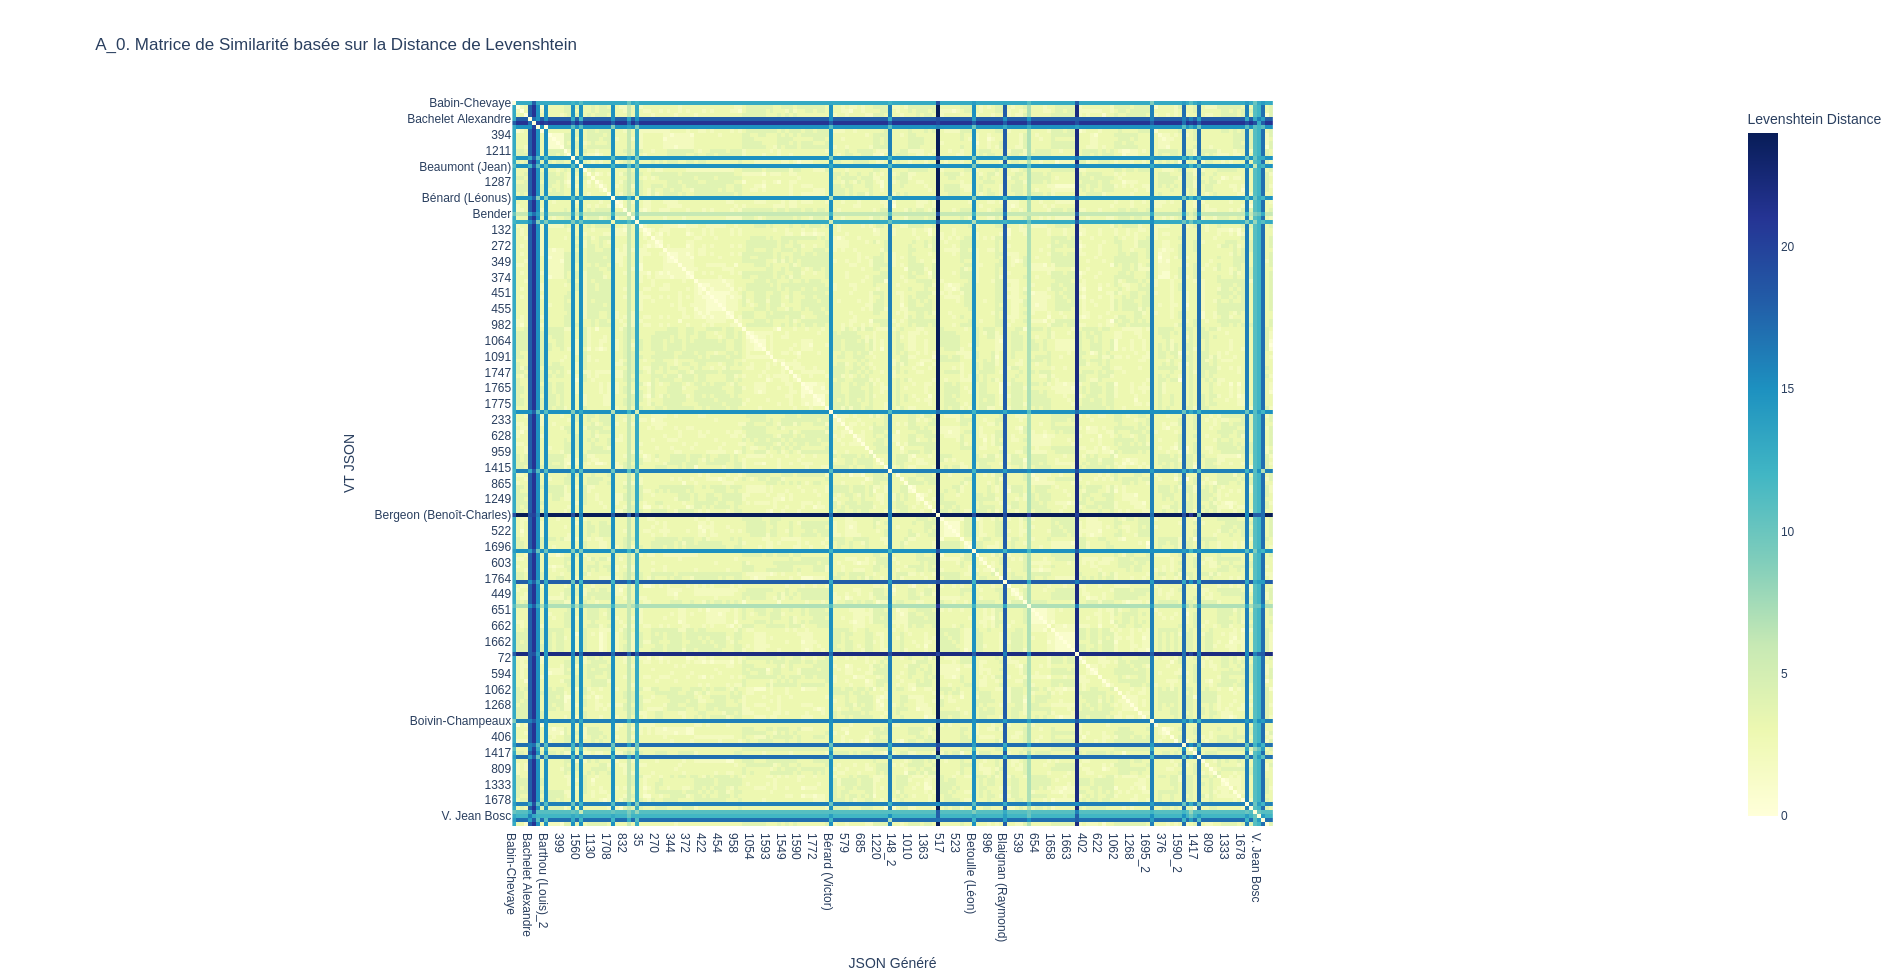
\includegraphics[width=\linewidth]{matricesim.png}
\caption{Matrice de similarité généré avec Python. Les points clairs représentent des distances faibles, c'est-à-dire des mots très similaires.}
\label{fig:matricesim}
\end{figure}

Ce dispositif visuel met en évidence des phénomènes difficiles à saisir autrement : comme les décalages -- des zones sombres signalent des omissions ou des décalages d’alignement, le modèle ayant « perdu le fil » avant de se resynchroniser -- et les regroupements -- des correspondances multiples sur une même ligne indiquent que plusieurs éléments ont été agrégés dans une seule entrée.

\begin{figure}[htbp]
\centering
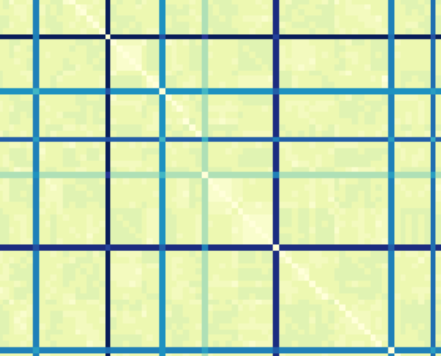
\includegraphics[width=\linewidth]{decalage.png}
\caption{Zoom sur la matrice de similarité : un décalage de la diagonale peut signifier une omission.}
\label{fig:decalage}
\end{figure}

L’observation de ces matrices ont d'ailleurs conduit, à la marge, à une réflexion plus conceptuelle. En effet, ces matrices ne forment pas toujours un espace métrique au sens strict, car des propriétés comme l’inégalité triangulaire peuvent être bafouées -- autrement dit, l'ensemble des distances peuvent dessiner un paysage impossible où il n'y a pas de cohérence avec les distances. Pourtant, on observe des zones de cohérence locale qui respectent suffisamment ces propriétés pour fonctionner comme des espaces métriques restreints. Là où il y a émergence de propriétés métriques, il y a l'hypothèse d'une correspondance entre la vérité terrain et les données générées. Deux ensembles identiques comparés forment un espace métrique : on pourrait alors calculer \enquote{l'effort} d'une matricité de similarité pour devenir un véritable espace métrique. Encore une fois, il s'agit d'une réflexion marginale qui n'a pas été développée ensuite. Cependant, cela permet de mettre en avant certains garde-fous dans le cadre de l'évaluation, à savoir le respect de certaines propriétés mathématiques liées à la mesure.

Ensuite reste l'étape de la comparaison proprement dite. Comment mettre correspondance les bonnes paires ? Comment comparer toutes les entrées de la vérité terrain avec celles générées ? Si la matrice de similarité représente toutes les relations entre les vérités terrain et les données générées, c'est une cartographie relationnelle qui ne nous permet pas d'apparier les ensembles en vue d'évaluer la qualité des prédictions; elle ne dit pas comment assembler nos entrées. De même, à cause des desynchronisation, il faut pouvoir aller comparer des éléments qui ne sont pas nécessairement \enquote{en-face}, c'est-à-dire qui ne partage pas le même rang.

Pour ce travail de mise en correspondance, intervient le transport optimal. Introduit par Gaspard Monge en 1781 -- dans son \emph{Mémoire sur la théorie des déblais et remblais} -- et reformulé par l'économiste soviétique Leonid Kantorovitch en 1942, le transport optimal vise à trouver la correspondance la plus économique entre deux ensembles : ici, les éléments de la vérité terrain et ceux générés. Plutôt que de tester toutes les permutations possibles, dont le nombre croît de manière factorielle, le transport optimal représente le problème sous forme d’une matrice de coût -- qui ici peut nous être donnée à partir de la matrice de similarité -- et cherche à minimiser la somme des coûts d’appariement. Cette méthode permet donc d’obtenir un alignement global optimal, même lorsque les ensembles ont des tailles différentes; de détecter les correspondances « justifiées » au sens du coût minimal, tout en identifiant les zones où la correspondance est faible ou artificielle; de dépasser une logique purement séquentielle pour analyser la distribution globale des erreurs et omissions. Notre coût, ici, ce sont les \enquote{coûts d'édition} autrement dit nos distances de Levenstein, exprimée par la matrice de similarité.

Cette approche est intéressante pour documenter l’état des sorties générées : elle ne prétend pas résoudre les problèmes d’ordre ou de sémantique, par exemple, apparier « sénateur » et « parlementaire » demanderait des distances sémantiques -- bien que c'est une piste envisageable avec les \emph{embeddings} dans le cas d'une analyse thématique des interventions parlementaires. En revanche, elle fournit une mesure robuste de dissemblance structurelle que nous offre justement le paysage des distances de Levenstein.En pratique, les vérifications manuelles réalisées sur de petits ensembles de données ont confirmé que les appariements identifiaient correctement les correspondances : chaque élément de la vérité terrain était relié à son équivalent prédit par le modèle. Ces tests ont permis d’esquisser un protocole d’évaluation fiable, en ancrant l’intuition dans des outils mathématiques et informatiques éprouvés.

Il ne s’agit cependant pas d’une démarche inédite : elle transpose à l’analyse des textes structurés un principe ancien et solide de l’évaluation de segmentation en vision par ordinateur. Comme l’explique Chazalon et Carlinet \footcite[][]{chazalon} à propos de la segmentation panoptique de cartes historiques, il est à la fois possible et pertinent de reformuler l’appariement des régions segmentées — contenus visuels — via un cadre bipartite, d’utiliser des métriques classiques (précision, rappel, F-score) \footcite[][]{chazalon}. Appliquée à nos données textuelles, cette approche inspire l’idée que l’appariement entre vérité terrain et données générées ne repose pas seulement sur le calcul statistique, mais peut aussi être qualifié, visualisé et interprété selon des logiques proches de celles de l’image numérique. En tout cas, une phase de l'expérimentation a consisté à comprendre la nature du transport optimal -- notamment avec les travaux de Gabriel Peyré \footcite[][]{peyre} -- afin d'en saisir les limites -- l'appariement ne regarde pas le sens des mots et ne prend pas compte de l'aspect séquentielle des entrées -- et les avantages -- permet justement de surmonter le problème des oublis et de faire correspondre des données qui ne sont pas \enquote{en face}. Cela impliquant ainsi d'intégrer \emph{a posteriori}, dans les métriques qui rendent compte de la qualité des données générées également la qualité de l'appariement.

Toutefois, ces expérimentations mettent également en évidence la dimension heuristique de cette démarche : les résultats dépendent autant du choix des mesures de similarité (distance de Levenshtein) que de la stratégie d’appariement retenue (transport optimal), ce qui engage une réflexion critique sur le design même de l’évaluation. Ainsi, même si la méthode hérite de protocoles éprouvés de l’imagerie, son adaptation à un contexte textuel demande des choix méthodologiques soigneux et explicités.

\section{Recouper des données pour l'analyse historienne}

Dans une perspective historienne, la capacité à naviguer dans les volumes du \emph{Journal officiel} ne repose pas uniquement sur la qualité des extractions textuelles, mais sur le recoupement systématique des données. L’enjeu est de relier des références issues des tables — ici limitées à des numéros de pages et aux occurences nominales — à des dates précises de publication, condition essentielle pour contextualiser les débats ou décisions mentionnés. Pour ce faire, nous avons exploité les manifests IIIF fournis par l’API Gallica, qui décrivent chaque volume sous forme d’une structure hiérarchisée : chaque page est identifiée, ordonnée et associée à une URL stable. Ce cadre technique permet de reconstituer un tableau complet \enquote{page → date}, en combinant l’ordre des pages du manifeste avec les métadonnées des volumes et les dates présentes sur les pages de titre. Cette opération ne vise pas à créer un modèle sophistiqué de reconnaissance ou d’indexation, mais plutôt à bâtir un pivot de référence déterministe pour toute analyse ultérieure : il devient possible de passer d’une citation brute (une page) à son contexte temporel exact. 

Il est important de souligner qu'à ce stade, cette correspondance se fonde sur les pages extraites par le système et rien n'indique que cette extraction repose sur des données fiables. Si ces données, à défaut d'évaluation, ne sont pas exploitables scientifiquement pour répondre à une question de recherche, il est cependant convenable de vérifier qu'on peut, à partir d'elles, avoir des informations plus intéressantes que des références de pages, comme des informations chronologiques.

\subsection{Des pages aux dates : utilisation de l'API Gallica et des métadonnées des manifestes}

La constitution d’un tableau « page → date » s’appuie sur les services IIIF proposés par Gallica, qui fournissent pour chaque document numérisé un manifest JSON décrivant l’ensemble de ses pages. Ce \emph{manifest} joue le rôle de table des matières numérique : il contient, pour chaque page, son ordre dans le volume, son libellé (numéro de page ou folio) et des identifiants pérennes vers l’image et le contenu OCRisé. La première étape consiste à interroger automatiquement cette ressource -- via des requêtes HTTP en lignes de commande, et notamment avec \enquote{curl} -- pour extraire la séquence complète des pages.

Ensuite, les pages sont indexées : chaque entrée du manifest est associée à son URL lisible et à son numéro de séquence. Cette structure séquentielle est cruciale, car elle fournit un pivot neutre pour relier des références issues d’autres sources (tables imprimées, index, etc.).

La seconde étape exploite les pages de titre qui portent la date d’édition. Ces informations, accessibles via l’API Gallica sont extraites puis assignées à des plages de pages contiguës : ainsi, toutes les pages comprises entre deux dates identifiées héritent de la date correspondante.

\begin{figure}[htbp]
\centering
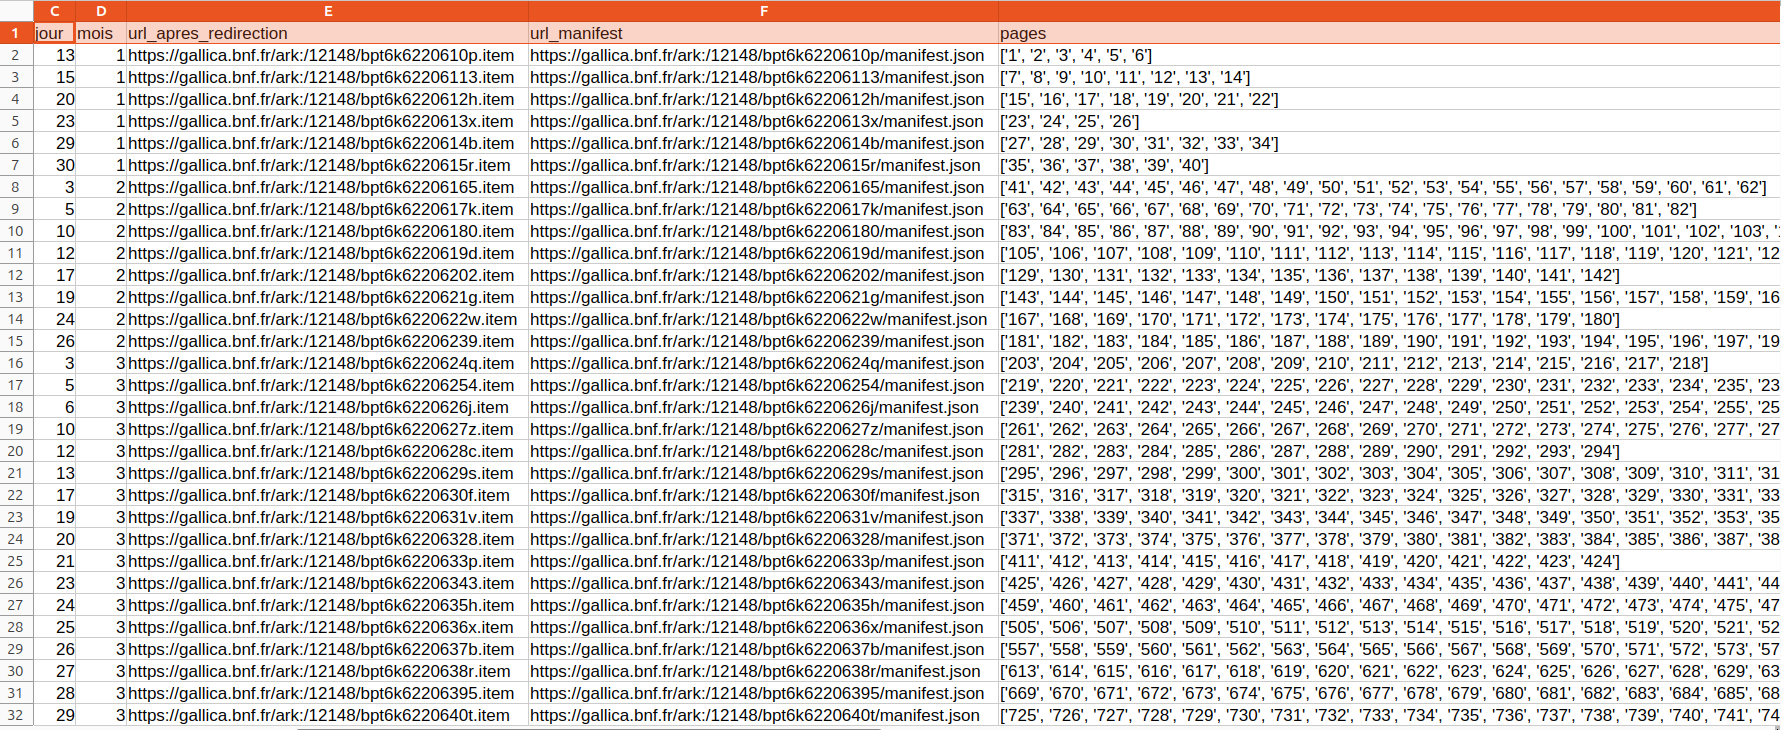
\includegraphics[width=\linewidth]{bnfjson.png}
\caption{Fragment du tableau de correspondance page/date en .csv}
\label{fig:bnfjson}
\end{figure}

En combinant ces deux sources (manifest + extraction de dates), on construit une table de correspondance exhaustive reliant chaque page d’un volume à sa date exacte de parution. Cette table, exportée en CSV, sert ensuite de base à des analyses historiennes : une référence de page extraite d’un index thématique peut être immédiatement replacée dans son contexte temporel. L’approche, entièrement automatisable, repose sur des standards ouverts (IIIF, JSON, HTTP) et sur des outils simples de parsing et de jointure de données, ce qui garantit sa robustesse et sa réutilisabilité. (ANNEXE 34)

\chapter{Livrables}

\section{Jeux de données pour le protocole d'évaluation de la sortie structurée}

\subsection{Protocole d’évaluation de la sortie structurée}

L’objectif de l’évaluation est de comparer les sorties produites par le LLM -- notées P, pour \emph{prédiction} -- au \emph{ground truth} -- la vérité terrain, notée G. Chaque instance de donnée correspond à une liste d’entrées, chacune constituée d’un nom d’orateur et d’une liste de pages référencées.

Un défi majeur, on l'a vu, tient au fait que le modèle peut produire le bon ensemble d’entrées, mais dans un ordre différent, ou avec de légères variations structurelles. Pour résoudre cela, nous adoptons une stratégie d’alignement flexible inspirée utilisant le transport optimal pour établir une correspondance \emph{one-to-one} entre prédictions et référence. Cette approche neutralise la contrainte d’ordre et tolère des divergences mineures, permettant une évaluation robuste.

L'OCRisation est indépendante et en amont de la comparaison :

\begin{enumerate}
\item Chaque page image est d’abord traitée indépendamment par le moteur OCR PERO pour détecter et transcrire le texte.
\item Compte tenu des difficultés persistantes de segmentation de mise en page, nous produisons trois variantes de transcription par page afin de refléter la variabilité de ce type de pipeline : une OCRisation \enquote{brute}, sans segmentation; une OCRisataion qui repose sur une segmentation manuelle; et une émulation d'une OCRisation réputée parfaite, fait à la main, qui correspond à la vérité terrain.

\end{enumerate}
Dans nos expérimentations, pour des raisons pratiques, chaque page est traitée indépendamment, mais la méthode peut être étendue à des contextes multi-pages.

Bien que les LLMs puissent être incités à générer des sorties structurées, il est essentiel de contraindre leurs générations au format attendu. Parmi les méthodes existantes, la plus efficace repose sur le filtrage des tokens valides au moment de l’inférence à l’aide d’un validateur externe (par exemple un automate fini). Cette capacité est disponible dans certaines API commerciales étendues.

Notre processus d’extraction s’appuie donc sur :

\begin{itemize}
\item un texte prétraité par OCR,
\item un schéma prédéfini (JSON),
\item un prompt naturel,
\item et une API supportant les sorties contraintes.

\end{itemize}
Pour cette étude, nous avons retenu l’API Mistral, avec le modèle \emph{Ministral 8B Instruct v2410}, en raison de ses bonnes performances \emph{zero-shot}, de son coût modéré et de la disponibilité publique de ses poids à des fins de recherche.

\subsection{Vérité terrain, prompt et schéma : un échantillon des Tables}

A l'issue de la démarche d'expérimentation en vue de l'évaluation a été produit le design de vérité terrain, accompagné de son schéma et du prompt, qui sera comparées à l'information extraite par le LLM. La tâche d’extraction repose sur l’identification des entrées individuelles dans les \emph{Tables nominatives} — c’est-à-dire les noms des sénateurs et leurs références de pages. (ANNEXE 33, 34)

Un échantillon aléatoire de cinq pages consécutives a été choisi pour transcription et annotation manuelles. Comme les entrées peuvent s’étendre sur plusieurs pages, certaines se retrouvent tronquées. Dans ces cas, le LLM a été explicitement instruit d’ignorer les éléments incomplets. Ce choix reflète les défis réalistes de l’extraction, où une prise en compte multi-pages (ou en flux continu) serait nécessaire en production, mais dépasse le cadre de cette étude.

L’évaluation porte sur 109 entrées réparties sur cinq pages, chacune testée dans les trois conditions OCR.

\subsection{Prédictions obtenues avec le modèle Mistral 8b avec  l'extraction guidée par schéma}

Pour l’année 1931, les \emph{Tables des noms} du Sénat couvrent 14 pages et comptent environ 300 entrées, chacune correspondant à une intervention en assemblée. Chaque entrée est associée à un orateur et détaille différents types d’actions (demandes d’interpellation, discussions de projets de loi, lecture de rapports de commission, dépôt d’amendements, etc.), accompagnées d’une référence de page renvoyant à la transcription complète de l’intervention.

Ces transcriptions sont publiées dans les \emph{Débats parlementaires} du Sénat. Les tables sont donc liées fonctionnellement aux transcriptions par la pagination. Comme la numérotation des pages est continue sur toute l’année, chaque référence permet de dater précisément l’intervention correspondante.

\section{Une métrique pour l'évaluation des données générées par la sortie stucturée via LLM}

\subsection{Mise en correspondance des prédictions et de la vérité terrain avec le transport optimal}

Pour comparer les entrées prédites et de référence, nous définissons une distance normalisée $d_e(g_i, p_j)$ qui combine deux composantes :

\begin{itemize}
\item \textbf{Nom de l’orateur (texte)} : distance de Ratcliff/Obershelp (basée sur la plus longue sous-chaîne commune), après minuscule et suppression des espaces. La distance normalisée $d_n(g_i, p_j) \in [0,1]$ vaut 0 pour un match exact et 1 pour une dissimilarité totale.

\item \textbf{Pages référencées (ensembles)} : distance Intersection-over-Union (IoU) :

\end{itemize}
$$
d_p(g_i, p_j) = 1 - \frac{|ref\_pages(g_i) \cap ref\_pages(p_j)|}{|ref\_pages(g_i) \cup ref\_pages(p_j)|}
$$

\begin{itemize}
\item \textbf{Distance d’entrée} :

\end{itemize}
$$
d_e(g_i, p_j) = d_n(g_i, p_j) \times d_p(g_i, p_j)
$$

Un appariement \emph{one-to-one} entre prédictions et vérité terrain est alors établi par transport optimal [19], minimisant la distance totale et fournissant une base rigoureuse pour l’évaluation.

\subsection{Limites des métriques classiques : précision, rappel et F1}

Les métriques usuelles (précision, rappel, F1) sont couramment utilisées pour évaluer les tâches d’extraction. Cependant, dans notre protocole, où les entrées sont alignées par transport optimal, elles deviennent trompeuses :

\begin{itemize}
\item l’appariement injectif force une correspondance complète, ce qui maximise artificiellement la précision,
\item le rappel ne reflète pas les entrées manquantes ou ajoutées,
\item la F1 hérite de ces biais et surestime les performances.

\end{itemize}
\subsection{Integrated Matching Quality (IMQ)}

Pour dépasser ces limites, nous exploitons directement la distance $d_e\$ pour définir un score de qualité \$q_i = 1 - d_e(g_i, p_i)$, qui reflète la proximité entre une entrée prédite et sa référence.

Plutôt que de fixer un seuil arbitraire pour décider du « bon » appariement, nous calculons la proportion de correspondances de qualité supérieure à un seuil $t\$, puis intégrons sur tout l’intervalle $[0,1]$ :

$$
IMQ = \int_0^1 F(t) \, dt
$$

où $F(t)\$ est la fraction des correspondances de qualité \$q_i \geq t$.

L’IMQ résume ainsi la qualité globale des appariements, récompensant à la fois leur nombre et leur proximité. Un score de 1 indique un alignement parfait. Cette métrique continue, indépendante de seuils arbitraires, est particulièrement adaptée aux sorties LLM, où de légères divergences sont fréquentes même sous fortes contraintes structurelles.

\subsection{Résultats et analyse}

Nous avons appliqué notre méthode d’appariement sur cinq pages distinctes (109 entrées), chacune traitée indépendamment et présentant des qualités OCR variables. Le tableau ci-dessous présente les résultats pour chaque page OCRisée sans segmentation ni correction, avec les tailles des ensembles de référence et prédits, ainsi que le nombre de correspondances retenues par transport optimal :

| Source  | Précision (biaisée) | Rappel (biaisé) | IMQ    | Entrées de référence | Entrées prédites | Correspondances |
| ------- | ------------------- | --------------- | ------ | -------------------- | ---------------- | --------------- |
| page 02 | 1.0000              | 0.9565          | 0.9059 | 23                   | 22               | 22              |
| page 03 | 1.0000              | 1.0000          | 0.8928 | 25                   | 25               | 25              |
| page 04 | 1.0000              | 1.0000          | 0.9591 | 19                   | 19               | 19              |
| page 05 | 1.0000              | 1.0000          | 0.8636 | 19                   | 19               | 19              |
| page 10 | 1.0000              | 1.0000          | 0.8193 | 23                   | 23               | 23              |

Toutes les pages affichent une précision et un rappel « biaisés » parfaits ; mais comme discuté en section précédente, ces métriques sont limitées car elles découlent directement de l’appariement injectif. Elles ne reflètent pas la qualité réelle des alignements.

L’\textbf{IMQ}, en revanche, fournit une évaluation plus fine, en capturant la distribution des qualités de correspondances. Pour toutes les pages traitées, les scores IMQ restent élevés (entre 0.8193 et 0.9591), montrant une homogénéité forte entre correspondances. L’IMQ évalue donc à la fois la complétude et la proximité sémantico-syntaxique des appariements, jouant un rôle hybride entre rappel qualitatif et précision pondérée.

 Variations entre pages

\emph{ \textbf{Pages 5 et 10} : IMQ plus bas, lié à des incohérences typographiques. De nombreux prénoms n’y sont pas mis entre parenthèses après le nom, contrairement à l’attendu dans le }ground truth* (21 \% des entrées sur la page 5, 39 \% sur la page 10). Cela augmente artificiellement la distance textuelle et dégrade la qualité perçue des correspondances.

\begin{itemize}
\item \textbf{Page 3} : malgré une précision/rappel parfaits, IMQ plus faible (0.8928), dû à des problèmes OCR causés par un pli dans la reliure, générant du bruit visuel.

\item \textbf{Page 2} : IMQ élevé (0.9059) malgré un rappel imparfait. Cela s’explique par un biais d’échantillonnage : le prompt avait été calibré sur cette page, ce qui améliore artificiellement la performance. Toutefois, les résultats solides sur la page 4 (IMQ = 0.9591) confirment la robustesse du dispositif.

\end{itemize}
Un cas particulier : sur la page 2, une personne est mentionnée deux fois (comme sénateur et comme ministre). Le \emph{ground truth} distingue ces deux entrées, tandis que le LLM les fusionne. Cela réduit artificiellement le rappel mais correspond à une rationalisation fonctionnelle du modèle.

 Comparaison avec OCR « parfait »

Lorsque l’on compare avec l’OCR jugé « parfait » (corrigé manuellement), les résultats s’améliorent globalement :

| Source  | Précision (biaisée) | Rappel (biaisé) | IMQ    | Entrées de référence | Entrées prédites | Correspondances |
| ------- | ------------------- | --------------- | ------ | -------------------- | ---------------- | --------------- |
| page 02 | 1.0000              | 1.0000          | 0.9513 | 23                   | 23               | 23              |
| page 03 | 1.0000              | 1.0000          | 0.9430 | 25                   | 25               | 25              |
| page 04 | 1.0000              | 1.0000          | 0.9821 | 19                   | 19               | 19              |
| page 05 | 1.0000              | 1.0000          | 0.8778 | 19                   | 19               | 19              |
| page 10 | 1.0000              | 1.0000          | 0.8966 | 23                   | 23               | 23              |

Dans certains cas, les versions OCR bruitées donnent des résultats paradoxalement meilleurs. Par exemple, les en-têtes courants capturés par l’OCR bruité fournissent un contexte utile pour les entrées tronquées en début de page. Ainsi, sur la page 2, le LLM a correctement reproduit la double mention (sénateur/ministre), alors que l’OCR corrigé ne l’a pas permis.

Cela montre que la performance dépend non seulement du LLM, mais aussi de l’adéquation entre ses comportements et la conception du \emph{ground truth}.

\begin{itemize}
\item Le prompt apparaît comme un paramètre critique : certains écarts ne sont pas liés au modèle, mais aux instructions données.
\item Un schéma de granularité raisonnable, couplé à un prompt générique, permet d’obtenir des résultats fiables sans nécessiter une connaissance « atomique » des spécificités documentaires.
\item L’analyse statistique page par page révèle des indices sur les exceptions structurelles internes aux documents (choix typographiques ou institutionnels), qui peuvent être significatives pour l’historien.

\end{itemize}
\section{Conclusion}

Ce travail a exploré l’utilisation des grands modèles de langage pour la génération de données structurées à partir de sources historiques, à travers une étude de cas centrée sur les \emph{Tables nominatives} du Sénat français de 1931. L’approche — combinant OCR, structuration guidée par schéma et génération contrainte via LLM — a produit des résultats évalués grâce à une métrique plus adaptée, l’\textbf{IMQ}, intégrée dans un protocole d’alignement optimal reliant données de référence et données prédites.

L’introduction de la métrique IMQ s’est révélée essentielle : elle permet d’évaluer la qualité de structuration au-delà des scores classiques de précision/rappel, inadéquats dans ce contexte.

Plusieurs pistes s’ouvrent pour renforcer la robustesse et la généralisation de l’approche :

\begin{itemize}
\item \textbf{Relier plus directement données extraites et questions de recherche} : il s’agit d’assurer que les hypothèses de réponse formulées à partir des données générées restent robustes dans le temps.
\item \textbf{Évaluer le prompt lui-même} : cette étape reste à formaliser pour parvenir à un protocole d’évaluation véritablement complet.
\item \textbf{Repenser la structuration de données} : elle ne doit pas être considérée comme un simple prétraitement neutre, mais comme un choix déterminant pour les analyses historiques possibles.

\end{itemize}
De ce point de vue, le prompt et le schéma de données apparaissent comme des \textbf{méta-paramètres} du système de production de données historiques. Leur génération et leur ajustement doivent être conçus comme faisant partie intégrante de la chaîne de traitement.

Une voie prometteuse consiste à \textbf{systématiser et automatiser ce processus de méta-optimisation}, afin de rendre ces approches reproductibles, transparentes et accessibles à des utilisateurs non spécialistes.

\begin{itemize}
\item Brown et al. → `\footcite[][]{brown}`

\item \footcite[][]{purentimeus}, \footcite[][]{poudra}, \footcite[][]{lamasse}, \footcite[][]{eugenedroitpol} \footcite[][]{saudrais} \footcite[][]{lemesle}, \footcite[][]{bonnard} \footcite[][]{coniez} \footcite[][]{morel} \footcite[][]{prost} \footcite[][]{coniez}

\item \footcite[][]{dirjo} \footcite[][]{jo1931} \footcite[][]{rygiel} \footcite[][]{gardey} \footcite[][]{boutier} \footcite[][]{comete} \footcite[][]{chazalon}\footcite[][]{com}\footcite[][]{comm}

\item Chen et al. → `\footcite[][]{chen}`

\item Clavert & Muller → `\footcite[][]{clavertmuller}`

\item Devlin et al. → `\footcite[][]{devlin}`

\item Finkel, Grenager & Manning → `\footcite[][]{finkelmanning}`

\item Humphries et al. → `\footcite[][]{humphries}`

\item Kirillov et al. → `\footcite[][]{kirillov}`

\item Kišš, Beneš & Hradiš → `\footcite[][]{kisshradis}`

\item Knutsen → `\footcite[][]{knutsen}`

\item Kodym & Hradiš → `\footcite[][]{kodymhradis}`

\item Kohút & Hradiš → `\footcite[][]{kohuthradis}`

\item Kojima et al. → `\footcite[][]{kojima}`

\item Liu et al. → `\footcite[][]{liu}`

\item de Marneffe et al. → `\footcite[][]{marneffe}`

\item Mintz et al. → `\footcite[][]{mintz}`

\item Mistral AI → `\footcite[][]{mistralai}`

\item Morel → `\footcite[][]{morel}`

\item Nadeau & Sekine → `\footcite[][]{nadeausekine}`

\item Peyré & Cuturi → ``

\item Radford et al. (2018) → `\footcite[][]{radford2018}`

\item Radford et al. (2019) → `\footcite[][]{radford2019}`

\item Wei et al. → `\footcite[][]{wei}`

\item Willard & Louf → `\footcite[][]{willardlouf}`

\item Yuan & Sester → `\footcite[][]{yuansester}`

\item Zhang & Shasha → `\footcite[][]{zhangshasha}`

\item Zhao et al. → `\footcite[][]{zhao}`
\end{itemize}




\part{Conclusion}

%%%%%%%%%%%%%%%%%%

\appendix %Des appendices: tables figures, etc

\chapter[Titre court]{Le titre très long de la première annexe}

%\input{fichier.tex}

\newpage{\pagestyle{empty}\cleardoublepage}

%%%%%%%%%%%%%%%%%%

\backmatter % glossaire, index, table des figures, table des matières.. (la bibliographie a déjà été appelée)

%\printindex
%\printglossaries[title=Glossaire]
%\listoftables
%\listoffigures
\tableofcontents
\end{document}
